\documentclass[12pt,t]{beamer}
\usepackage{graphicx}
\usepackage{amsmath,amssymb}
\usepackage{colortbl}

\setbeameroption{hide notes}
\setbeamertemplate{note page}[plain]

% get rid of junk
\usetheme{default}
\beamertemplatenavigationsymbolsempty
\hypersetup{pdfpagemode=UseNone} % don't show bookmarks on initial view

% font
%\usepackage{fontspec}
%\setsansfont{TeX Gyre Heros}
%\setbeamerfont{note page}{family*=pplx,size=\footnotesize} % Palatino for notes
% "TeX Gyre Heros can be used as a replacement for Helvetica"
% In Unix, unzip the following into ~/.fonts
% In Mac, unzip it, double-click the .otf files, and install using "FontBook"
%   http://www.gust.org.pl/projects/e-foundry/tex-gyre/heros/qhv2.004otf.zip

% named colors
\definecolor{offwhite}{RGB}{249,242,215}
\definecolor{foreground}{RGB}{255,255,255}
\definecolor{background}{RGB}{24,24,24}
\definecolor{title}{RGB}{107,174,214}
\definecolor{gray}{RGB}{155,155,155}
\definecolor{subtitle}{RGB}{102,255,204}
\definecolor{hilight}{RGB}{102,255,204}
\definecolor{vhilight}{RGB}{255,111,207}
\definecolor{lolight}{RGB}{155,155,155}
%\definecolor{green}{RGB}{125,250,125}
\definecolor{pink}{HTML}{FC0964}
\definecolor{orange}{HTML}{FD971F}
\definecolor{blue}{HTML}{66D9EF}
\definecolor{green}{HTML}{7FB347}


% use those colors
\setbeamercolor{titlelike}{fg=title}
\setbeamercolor{subtitle}{fg=subtitle}
\setbeamercolor{institute}{fg=gray}
\setbeamercolor{normal text}{fg=foreground,bg=background}
\setbeamercolor{item}{fg=foreground} % color of bullets
\setbeamercolor{subitem}{fg=gray}
\setbeamercolor{itemize/enumerate subbody}{fg=gray}
\setbeamertemplate{itemize subitem}{{\textendash}}
\setbeamerfont{itemize/enumerate subbody}{size=\footnotesize}
\setbeamerfont{itemize/enumerate subitem}{size=\footnotesize}

% page number
\setbeamertemplate{footline}{%
    \raisebox{5pt}{\makebox[\paperwidth]{\hfill\makebox[20pt]{\color{gray}
          \scriptsize\insertframenumber}}}\hspace*{5pt}}

% add a bit of space at the top of the notes page
\addtobeamertemplate{note page}{\setlength{\parskip}{12pt}}

% a few macros
\newcommand{\bi}{\begin{itemize}}
\newcommand{\ei}{\end{itemize}}
\newcommand{\ig}{\includegraphics}
\newcommand{\subt}[1]{{\footnotesize \color{subtitle} {#1}}}

% title info
\title{Introduction to Radial Basis Function Method}
\subtitle{How to Interpolate Scattered Data with Radial Basis}
\author{\href{https://github.com/jessebett/}{Jesse Bettencourt}}
\institute{McMaster University\\Dr. Kevlahan}
\date{\href{jessebett@gmail.com}{\tt \scriptsize jessebett@gmail.com}
\\[-4pt]
\href{http://github.com/jessebett}{\tt \scriptsize github.com/jessebett}
}

\graphicspath{{./Images/}}


\begin{document}

% title slide
\setbeamertemplate{footline}{} % no page number here
\begin{frame}
  \titlepage
  \note{}
\end{frame}

\begin{frame}{Motivation}
Given a set of measurements \textcolor{pink}{$\{f_i\}_{i=1}^N$}
taken at corresponding data sites \textcolor{orange}{$\{x_i\}_{i=1}^N$}
we want to find an interpolation function \textcolor{blue}{$s(x)$}
that informs us on our system at locations different from our data sites.\\
\bigskip 

\begin{figure}
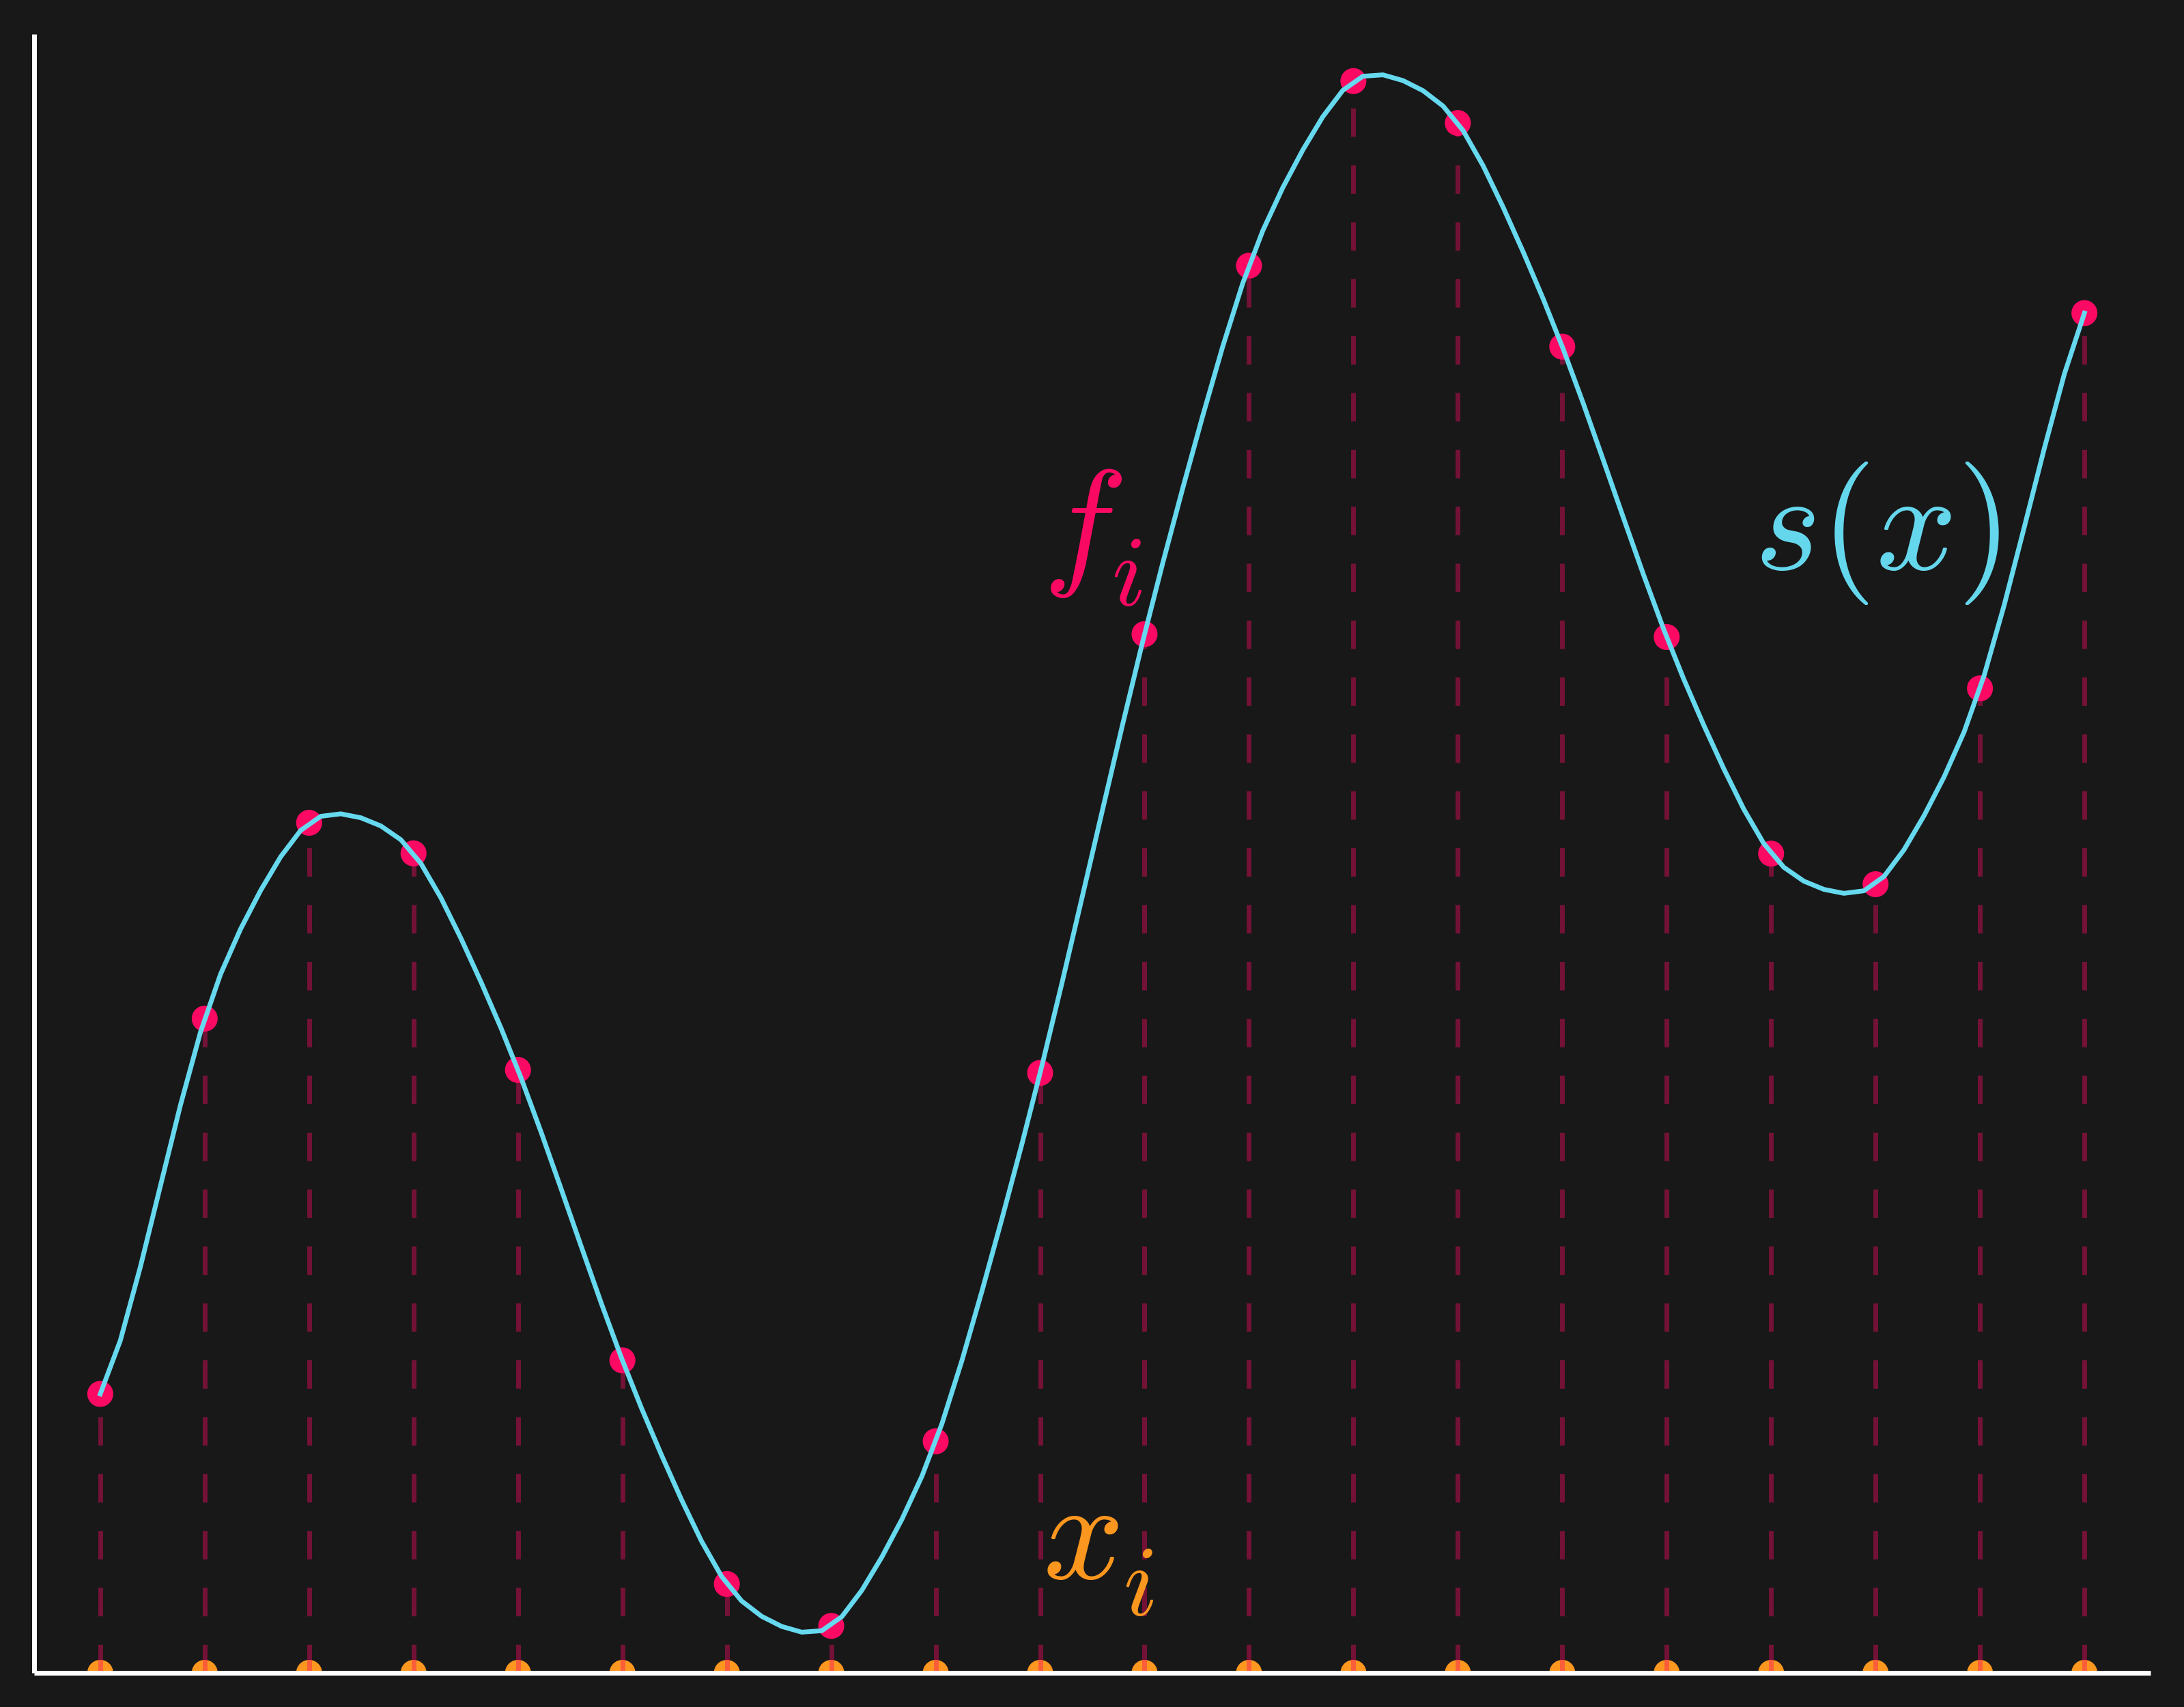
\includegraphics[width=0.7\textwidth, keepaspectratio]{fig1.png}
\end{figure}

\note{}
\end{frame}
\begin{frame}{Motivation}
Given a set of measurements \textcolor{pink}{$\{f_i\}_{i=1}^N$}
taken at corresponding data sites \textcolor{orange}{$\{x_i\}_{i=1}^N$}
we want to find an interpolation function \textcolor{blue}{$s(x)$}
that informs us on our system at locations different from our data sites.\\
\bigskip 

\subt{Examples of Data Sites and Measurments}
\begin{itemize}
\item[1D:] A series of temperature measurements over a time period
\item[2D:] Surface temperature of a lake based on measurements collected at sample surface locations 
\item[3D:] Distribution of temperature within a lake
\item[n-D:] Machine learning, financial models, system optimization
\end{itemize}

\note{}
\end{frame}

\begin{frame}{What makes a good fit?}
\bi
\item \textcolor{orange}{Interpolation}: $s(x)$ \subt{exactly matches} our measurements at our data sites. \\ 
\item \textcolor{green}{Approximation}: $s(x)$ \subt{closely matches} our measurements at our data sites, e.g. with Least Squares 
\ei
\begin{figure}
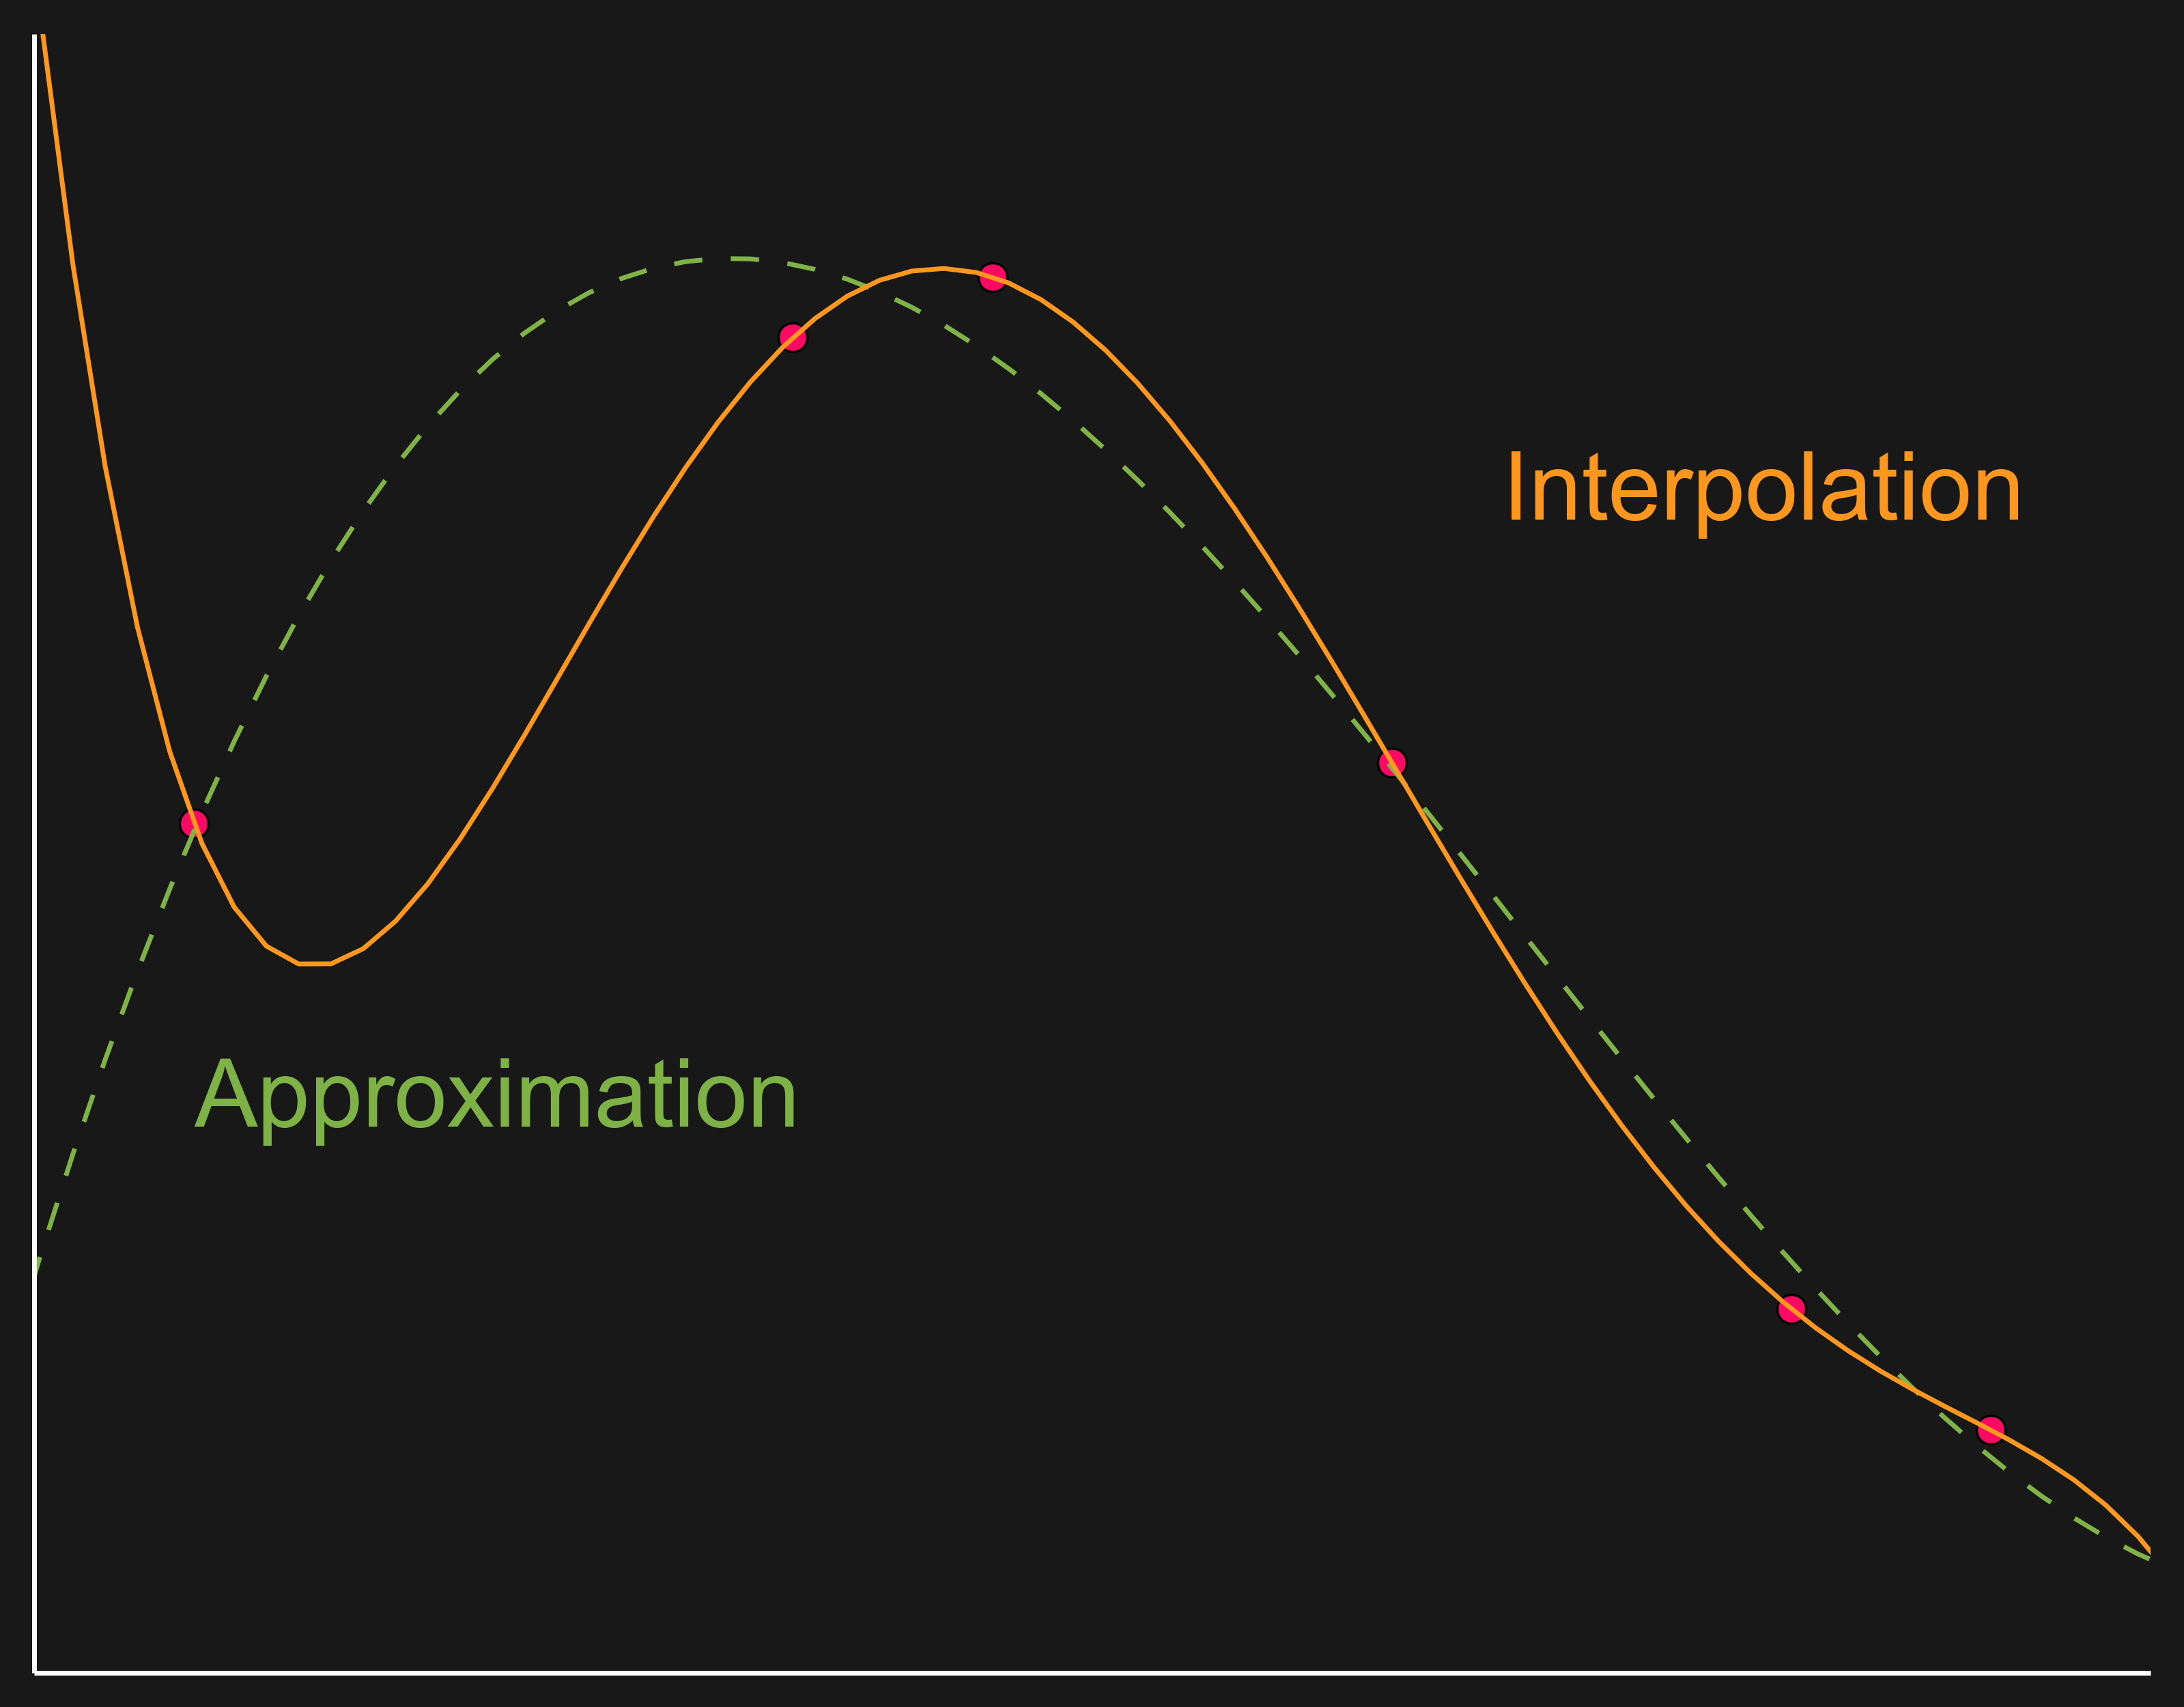
\includegraphics[width=0.7\textwidth, keepaspectratio]{fig2.png}
\end{figure}

\note{}
\end{frame}

\begin{frame}{For today's purposes...}
we will only consider interpolation.

\bi
\item Interpolation: $\textcolor{blue}{s(\textcolor{orange}{x_i})}=\textcolor{pink}{f_i}$ $\forall i\in\{0 \mathellipsis N \}$
\ei
\begin{figure}
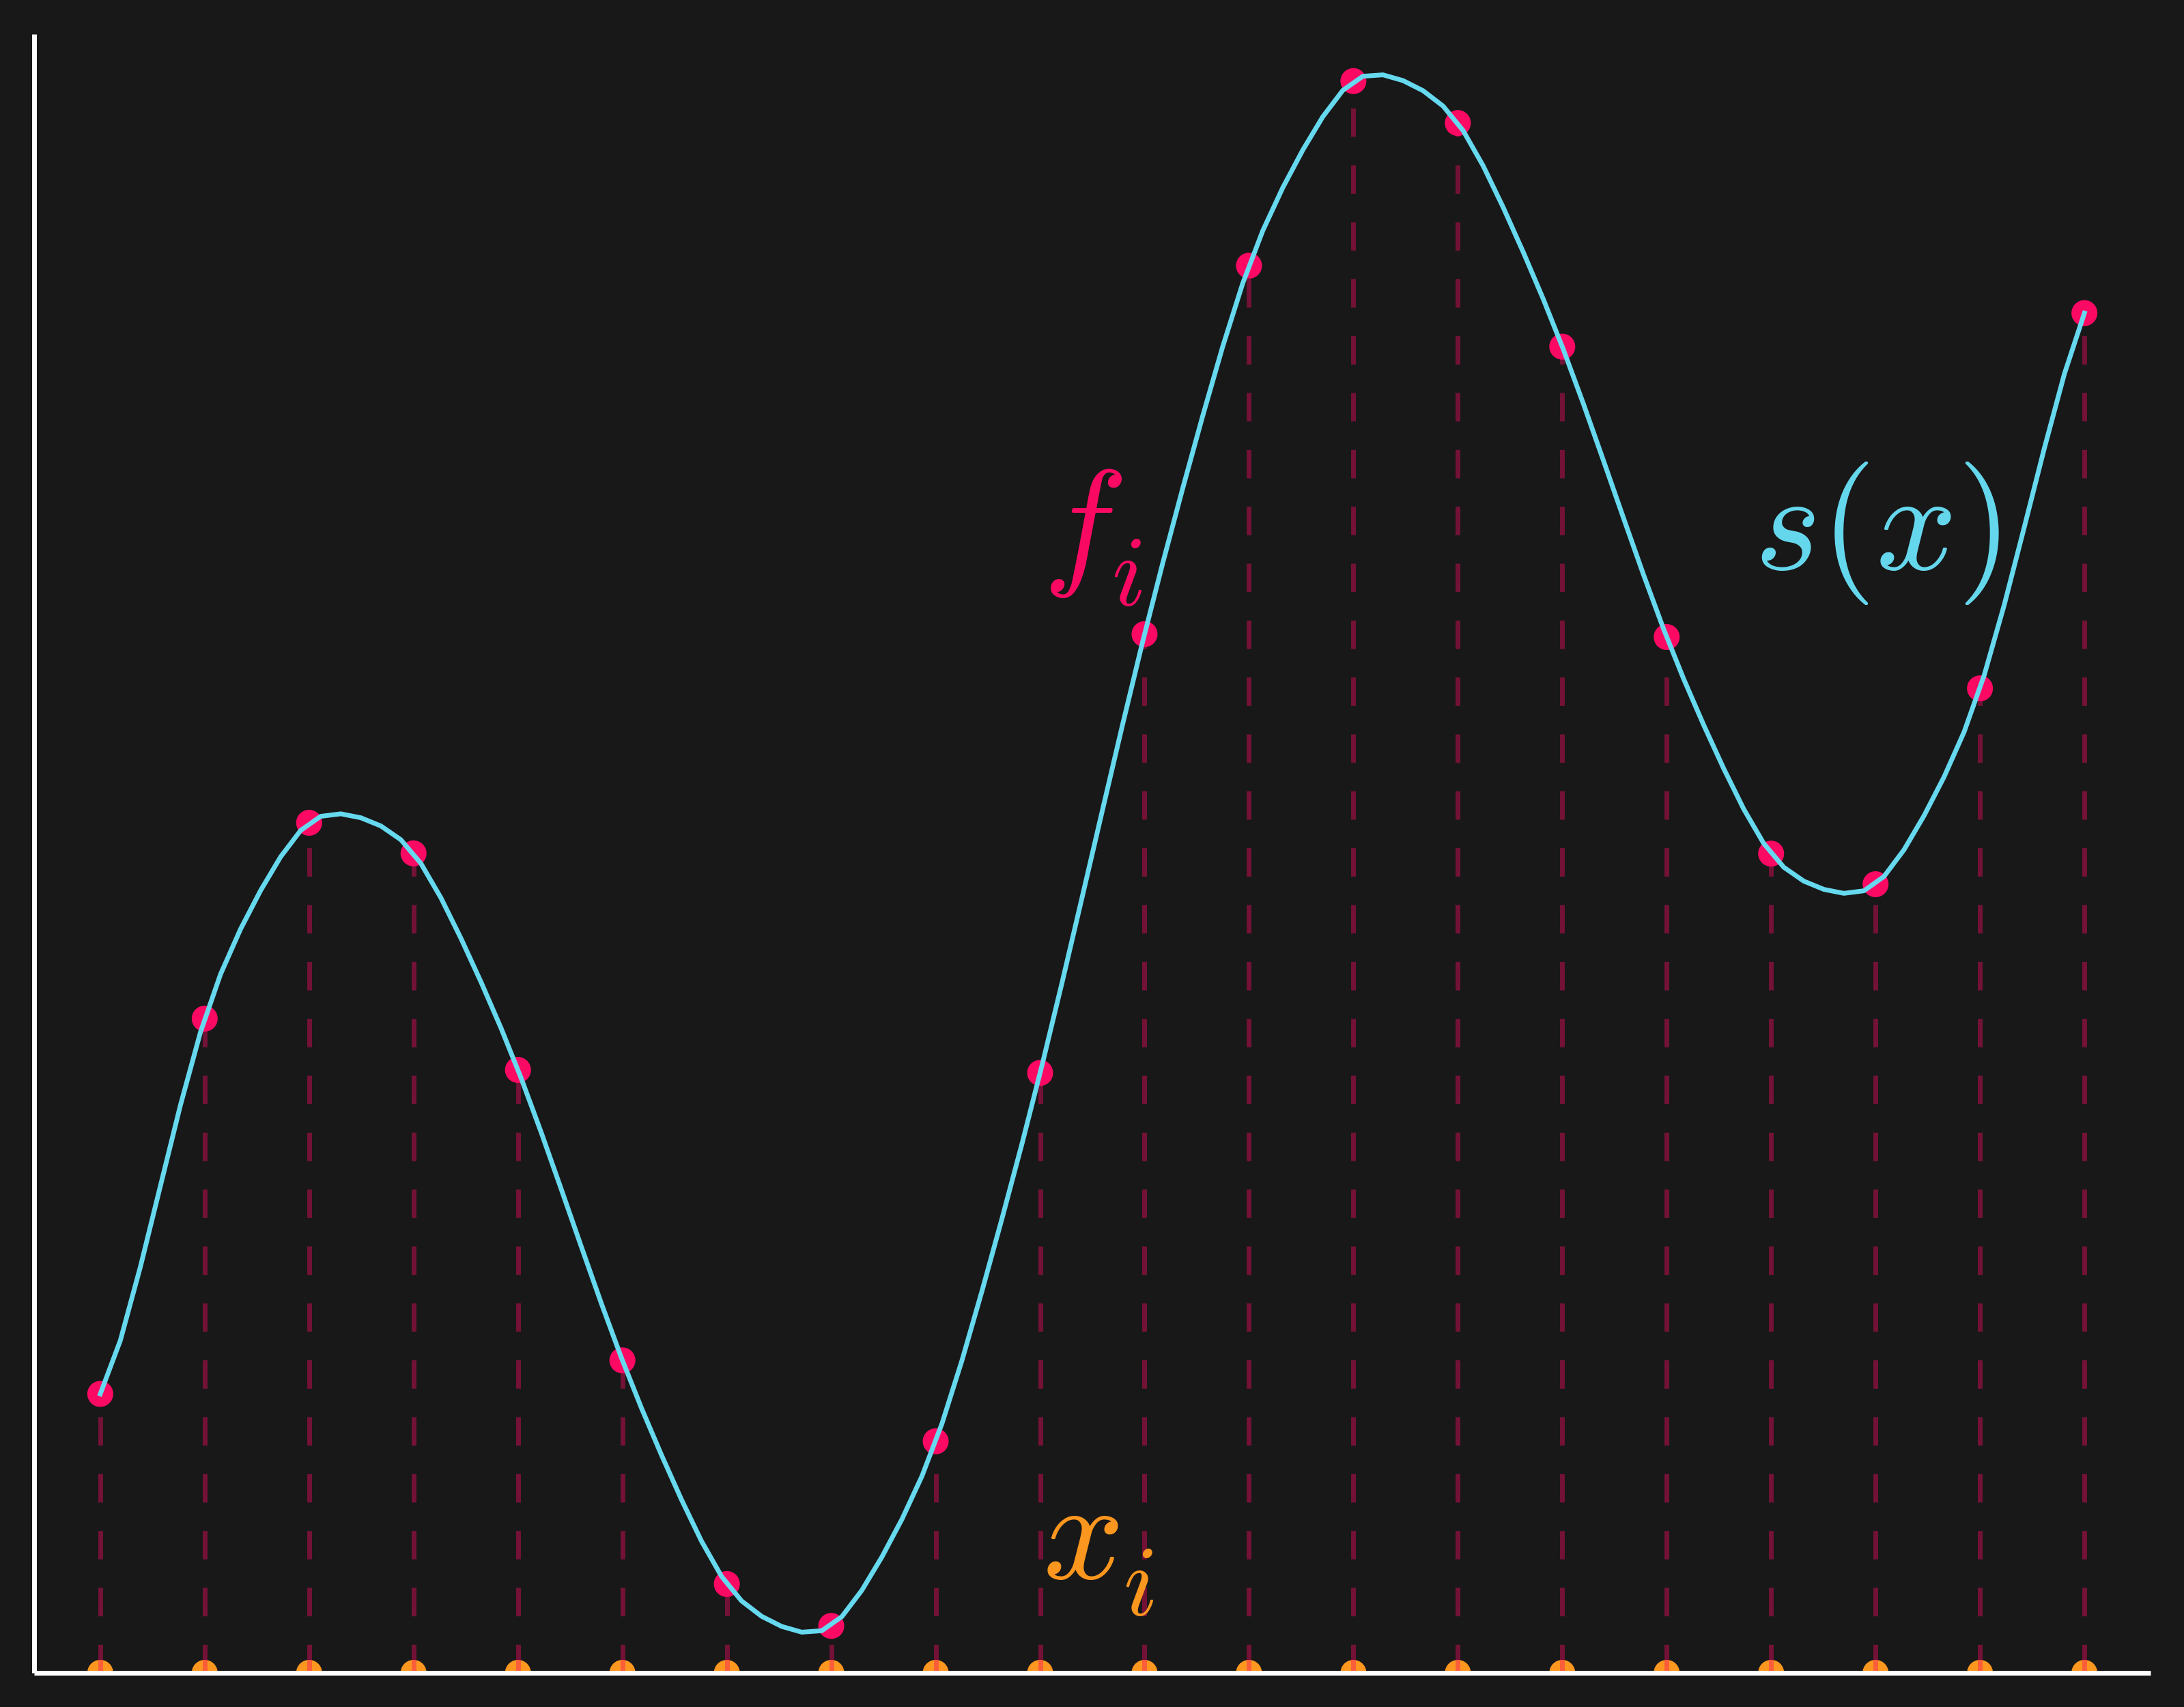
\includegraphics[width=0.7\textwidth, keepaspectratio]{fig1.png}
\end{figure}


\note{}
\end{frame}

\begin{frame}[c]{Our Problem, Restated}

\subt{Interpolation of Scattered Data}

Given data $(\textcolor{orange}{x_i},\textcolor{pink}{f_i})$, $i=1, \mathellipsis, N$, such that $\textcolor{orange}{x_i} \in \mathbb{R}^n$, $\textcolor{pink}{f_i} \in \mathbb{R}$, we want to find a continuous function $\textcolor{blue}{s(x)}$ such that $\textcolor{blue}{s(\textcolor{orange}{x_i})}=\textcolor{pink}{f_i}$ $\forall i\in\{0 \mathellipsis N \}$

\begin{figure}
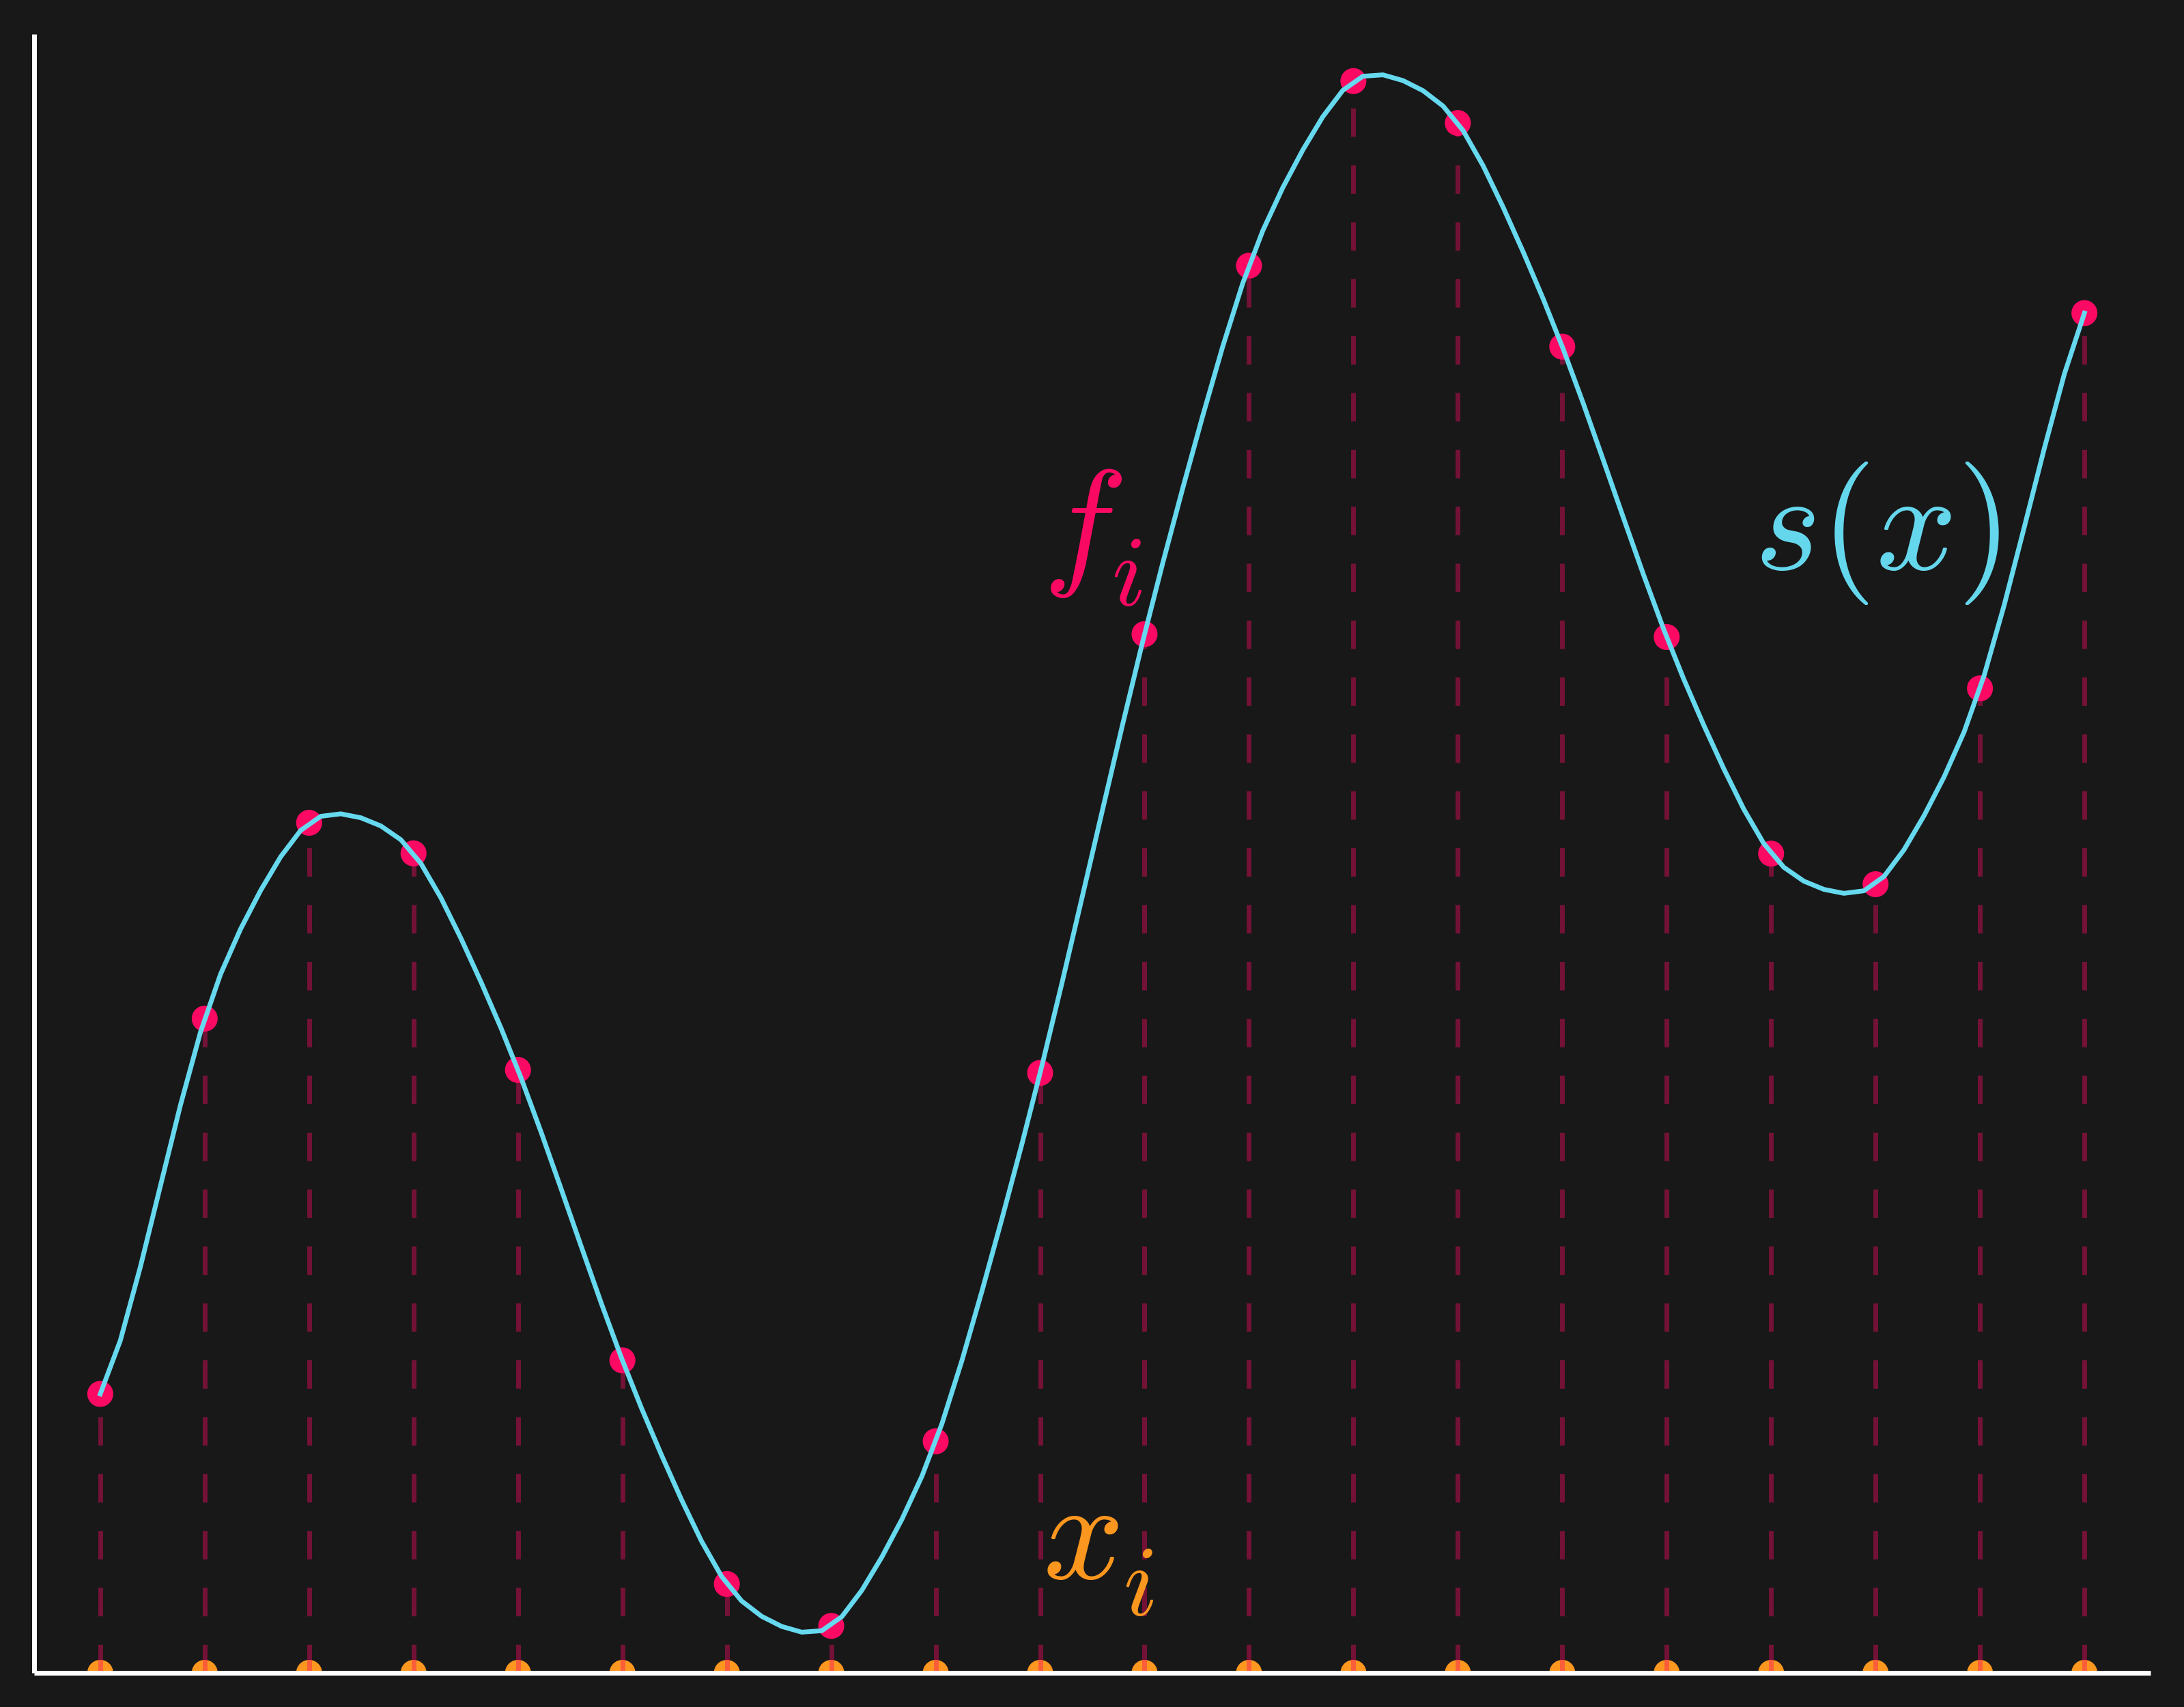
\includegraphics[width=0.7\textwidth, keepaspectratio]{fig1.png}
\end{figure}

\note{}
\end{frame}

\begin{frame}{A Familiar Approach}
\subt{Convenient Assumtption}

Assume $s(x)$ is a linear combination of \subt{basis functions} $\psi_i$
\begin{center}
$s(x)=\sum_{i=1}^N \lambda_i \psi_i$
\end{center}
\pause
\subt{Interpolation as a Linear System}

Following this assumption we have a system of linear equations
\begin{center}
$A\boldsymbol{\lambda}=\boldsymbol{f}$
\end{center}
 where
 \bi
\item[A] is called the \subt{interpolation matrix} whose entries are given by\\
\begin{align*}
a_{ij}&=\psi_j(x_i) & i,j= 1 \mathellipsis N\\
\intertext{and}
\boldsymbol{\lambda} &=\left[ \lambda_1, \mathellipsis, \lambda_N \right]^T\\
\boldsymbol{f} &=\left[ f_1, \mathellipsis, f_N \right]^T
\end{align*}
% \item[$\boldsymbol{\lambda}$] $=\left[ \lambda_1, \mathellipsis, \lambda_N \right]^T$
% \item[$\boldsymbol{f}$] $=\left[ f_1, \mathellipsis, f_N \right]^T$
\ei

\note{}
\end{frame}

\begin{frame}{The Well-Posed Problem}
\begin{center}
$A\boldsymbol{\lambda}=\boldsymbol{f}$
\end{center}

Solving this linear system, thus finding $s(x)$, is only possible if the problem \subt{well-posed}, i.e., $\exists$ a unique solution 
\bigskip
\pause

\subt{Result from introductory linear algebra:} 

The problem will be well-posed if and only if the interpolation matrix A is \subt{non-singular}, i.e., $\det(A)\neq0$.
\bigskip
\pause

\subt{Note:} The non-singularity of A will depend on our choice of basis functions, $\psi_{i=1}^N$

\note{INCLUDE WELL-Conditioned Here!}
\end{frame}

\begin{frame}{Easily Well-Posed in 1D}
In 1D, many choices of basis functions will guarantee a well-posed problem as long as the data-sites are distinct. 
\bigskip
\pause

\subt{Example}

We are familiar with \subt{polynomial interpolation}, interpolating from N data sites with a $(N-1)$-degree polynomial. 
\begin{center}
$\psi_{i=1}^N=\{1,x,x^2,x^3, \mathellipsis, x^{N-1}\}$
\end{center}
\pause
\begin{figure}
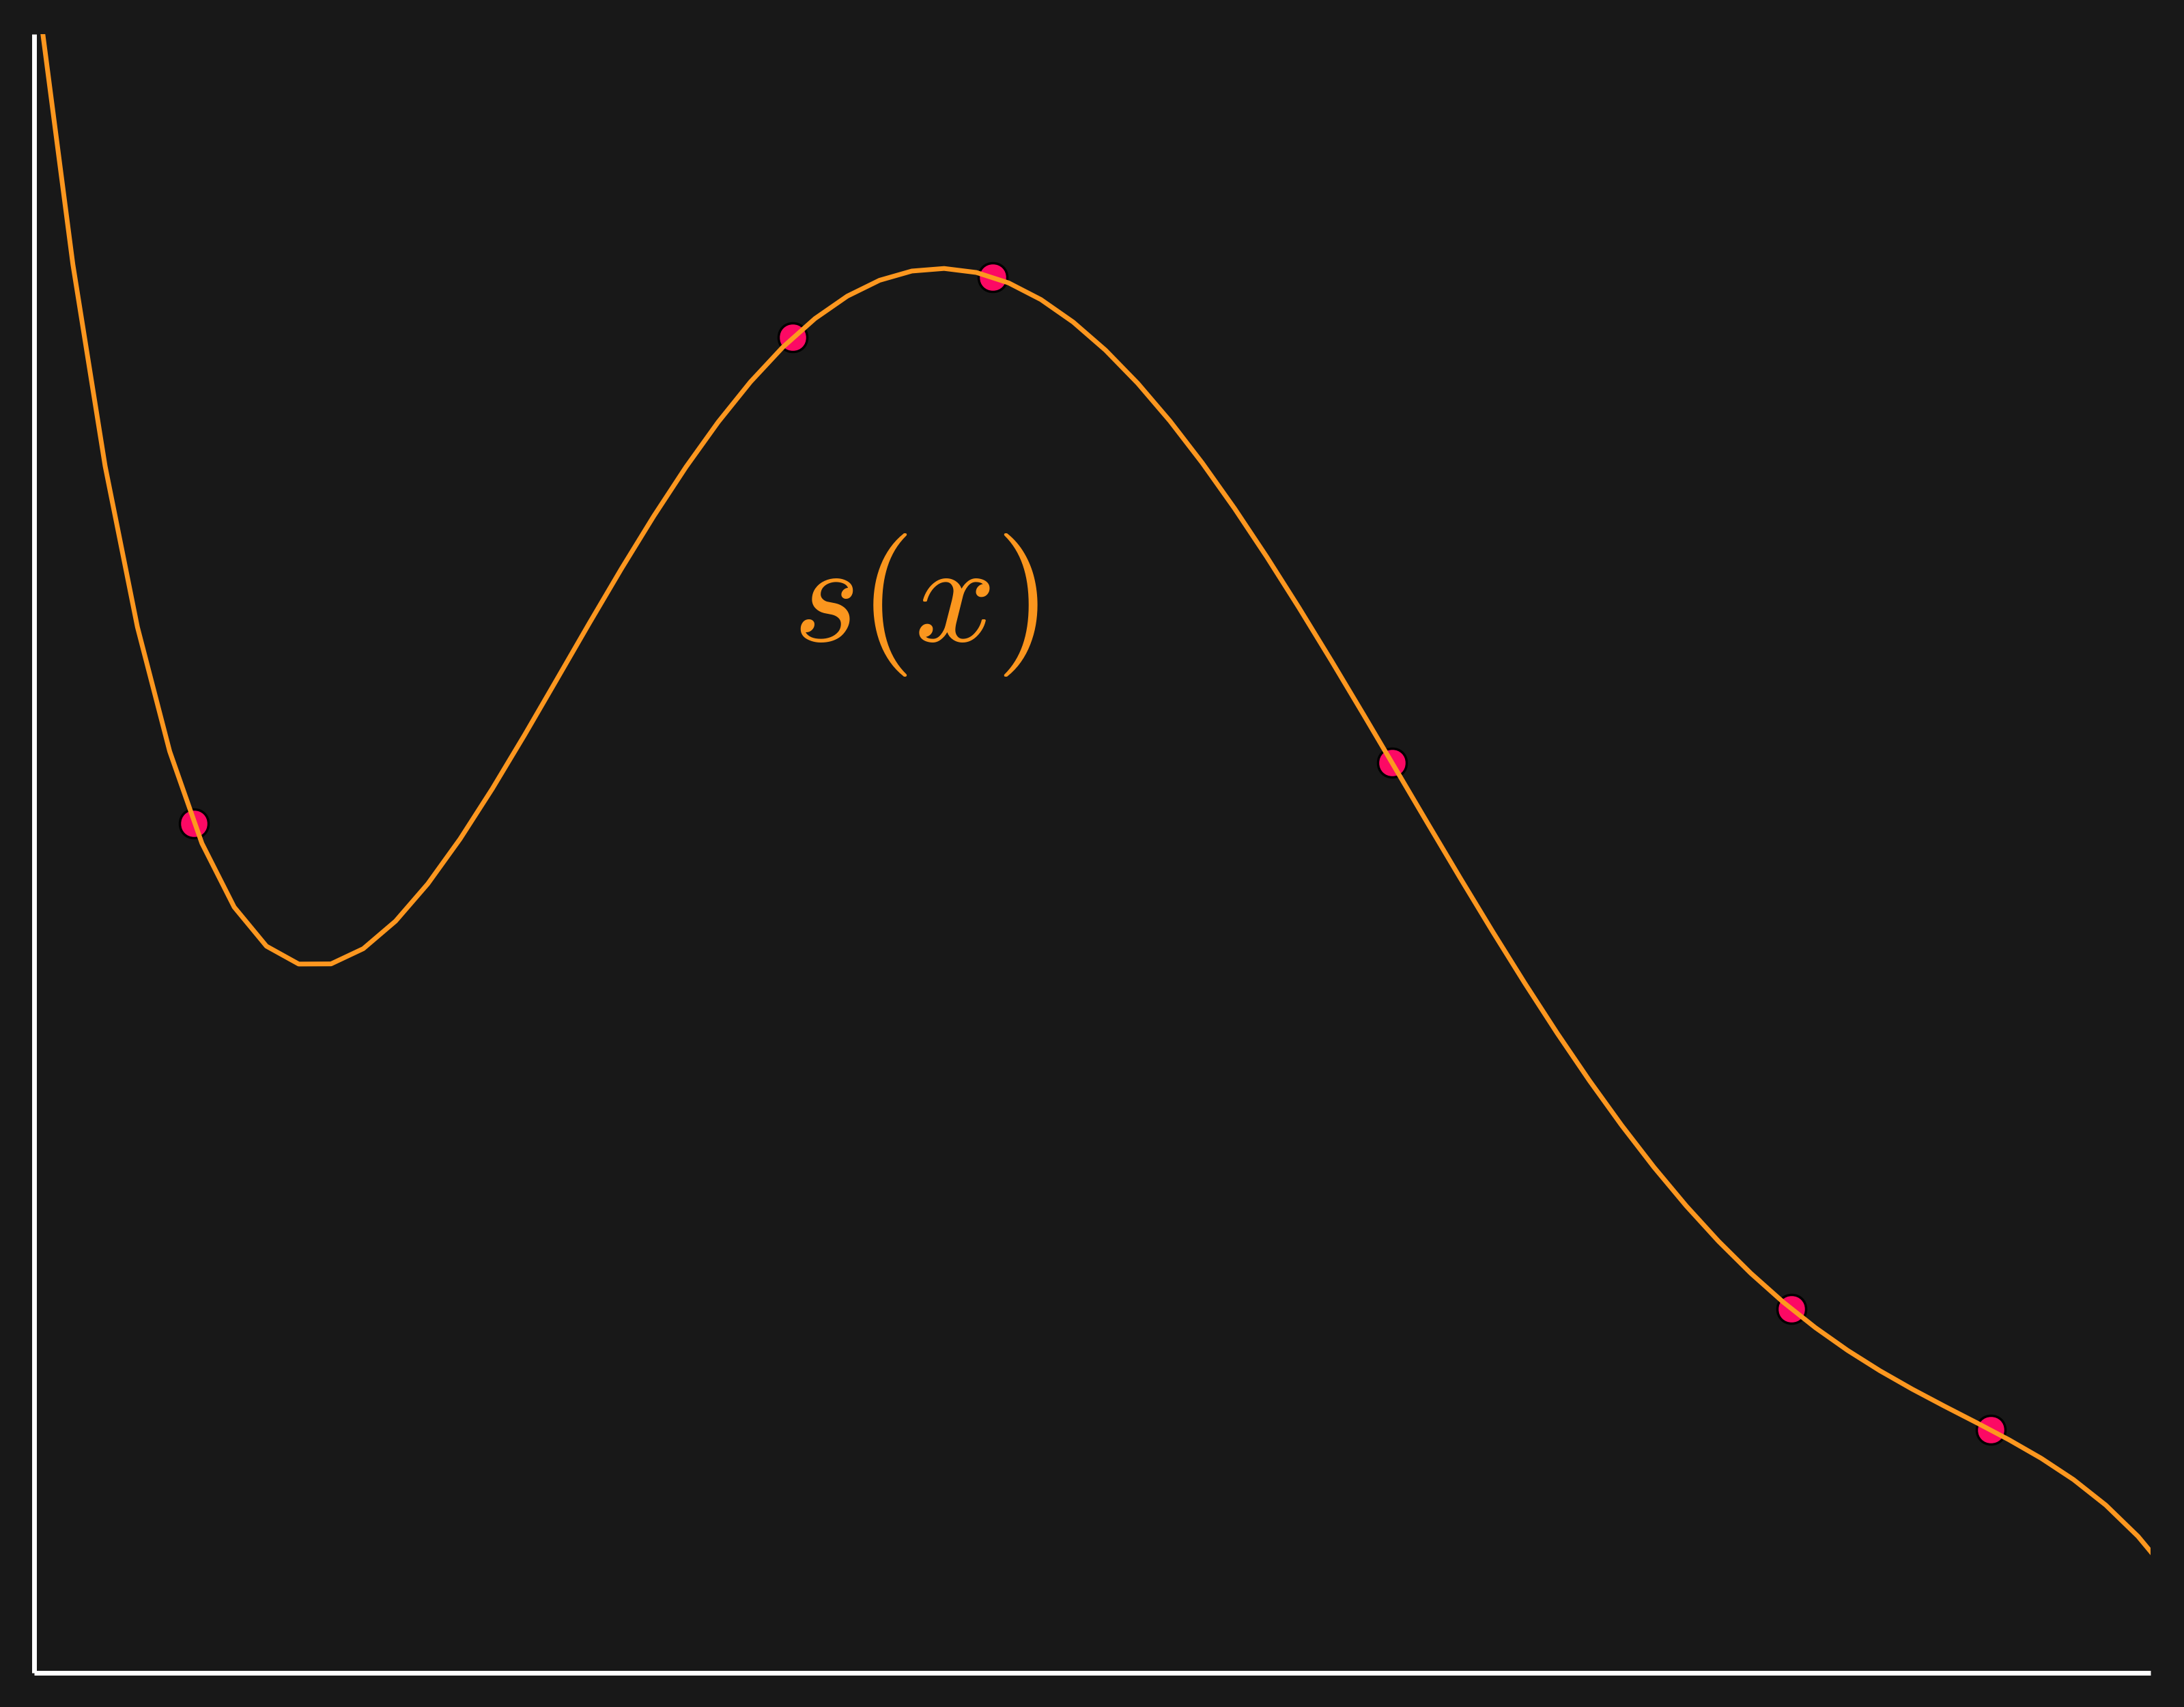
\includegraphics[width=0.4\textwidth, keepaspectratio]{fig3.png}
\end{figure}
\footnotesize{\textcolor{orange}{$s(x)=-0.02988 x^5 + 0.417 x^4 - 2.018 x^3 + 3.694 x^2 - 1.722 x - 5.511e^{-14}$}}
\note{}
\end{frame}

\begin{frame}{A Problem in Higher Dimensions}
For n-Dimensions where $n\geq 2$ there is no such guarantee.
\bigskip
\pause

For any set of basis functions, $\psi_{i=1}^N$ (chosen independently of the data sites) $\exists$ a set of distinct data sites $\{x_i\}_{i=1}^N$
such that the interpolation matrix becomes singular. 
\bigskip
\pause

\subt{Implication:}
If we choose our basis functions independently of the data, we are not guaranteed a well-posed problem.
\bigskip

\pause
\subt{Note:}
This results from the Haar-Mairhuber-Curtis Theorem
\begin{figure}[!htb]
\minipage{0.25\textwidth}
  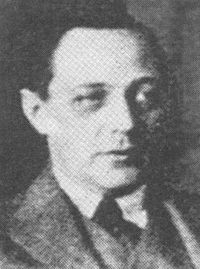
\includegraphics[width=\linewidth]{Haar.jpg}
\endminipage\hfill
\minipage{0.25\textwidth}
  
\includegraphics[width=\linewidth]{Mairhuber-crop.jpg}
\endminipage\hfill
\minipage{0.25\textwidth}%
  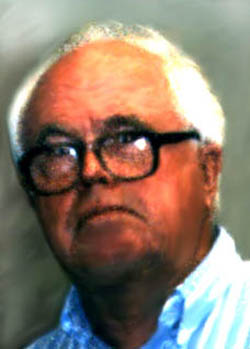
\includegraphics[width=\linewidth]{Curtis.jpg}
\endminipage
\end{figure}


\note{}
\end{frame}

\begin{frame}[c]{A Solution in Higher Dimensions}
\subt{Implication:}
If we choose our basis functions independently of the data, we are not guaranteed a well-posed problem.
\bigskip

\subt{Solution?}
\pause
Choose basis functions depending on the data!
\bigskip

\note{}
\end{frame}

\begin{frame}{Basis Functions Depending on Data}
First, consider what we call the \subt{basic function}\\
\begin{equation*}
\psi(x)=|x|
\end{equation*}

\begin{figure}
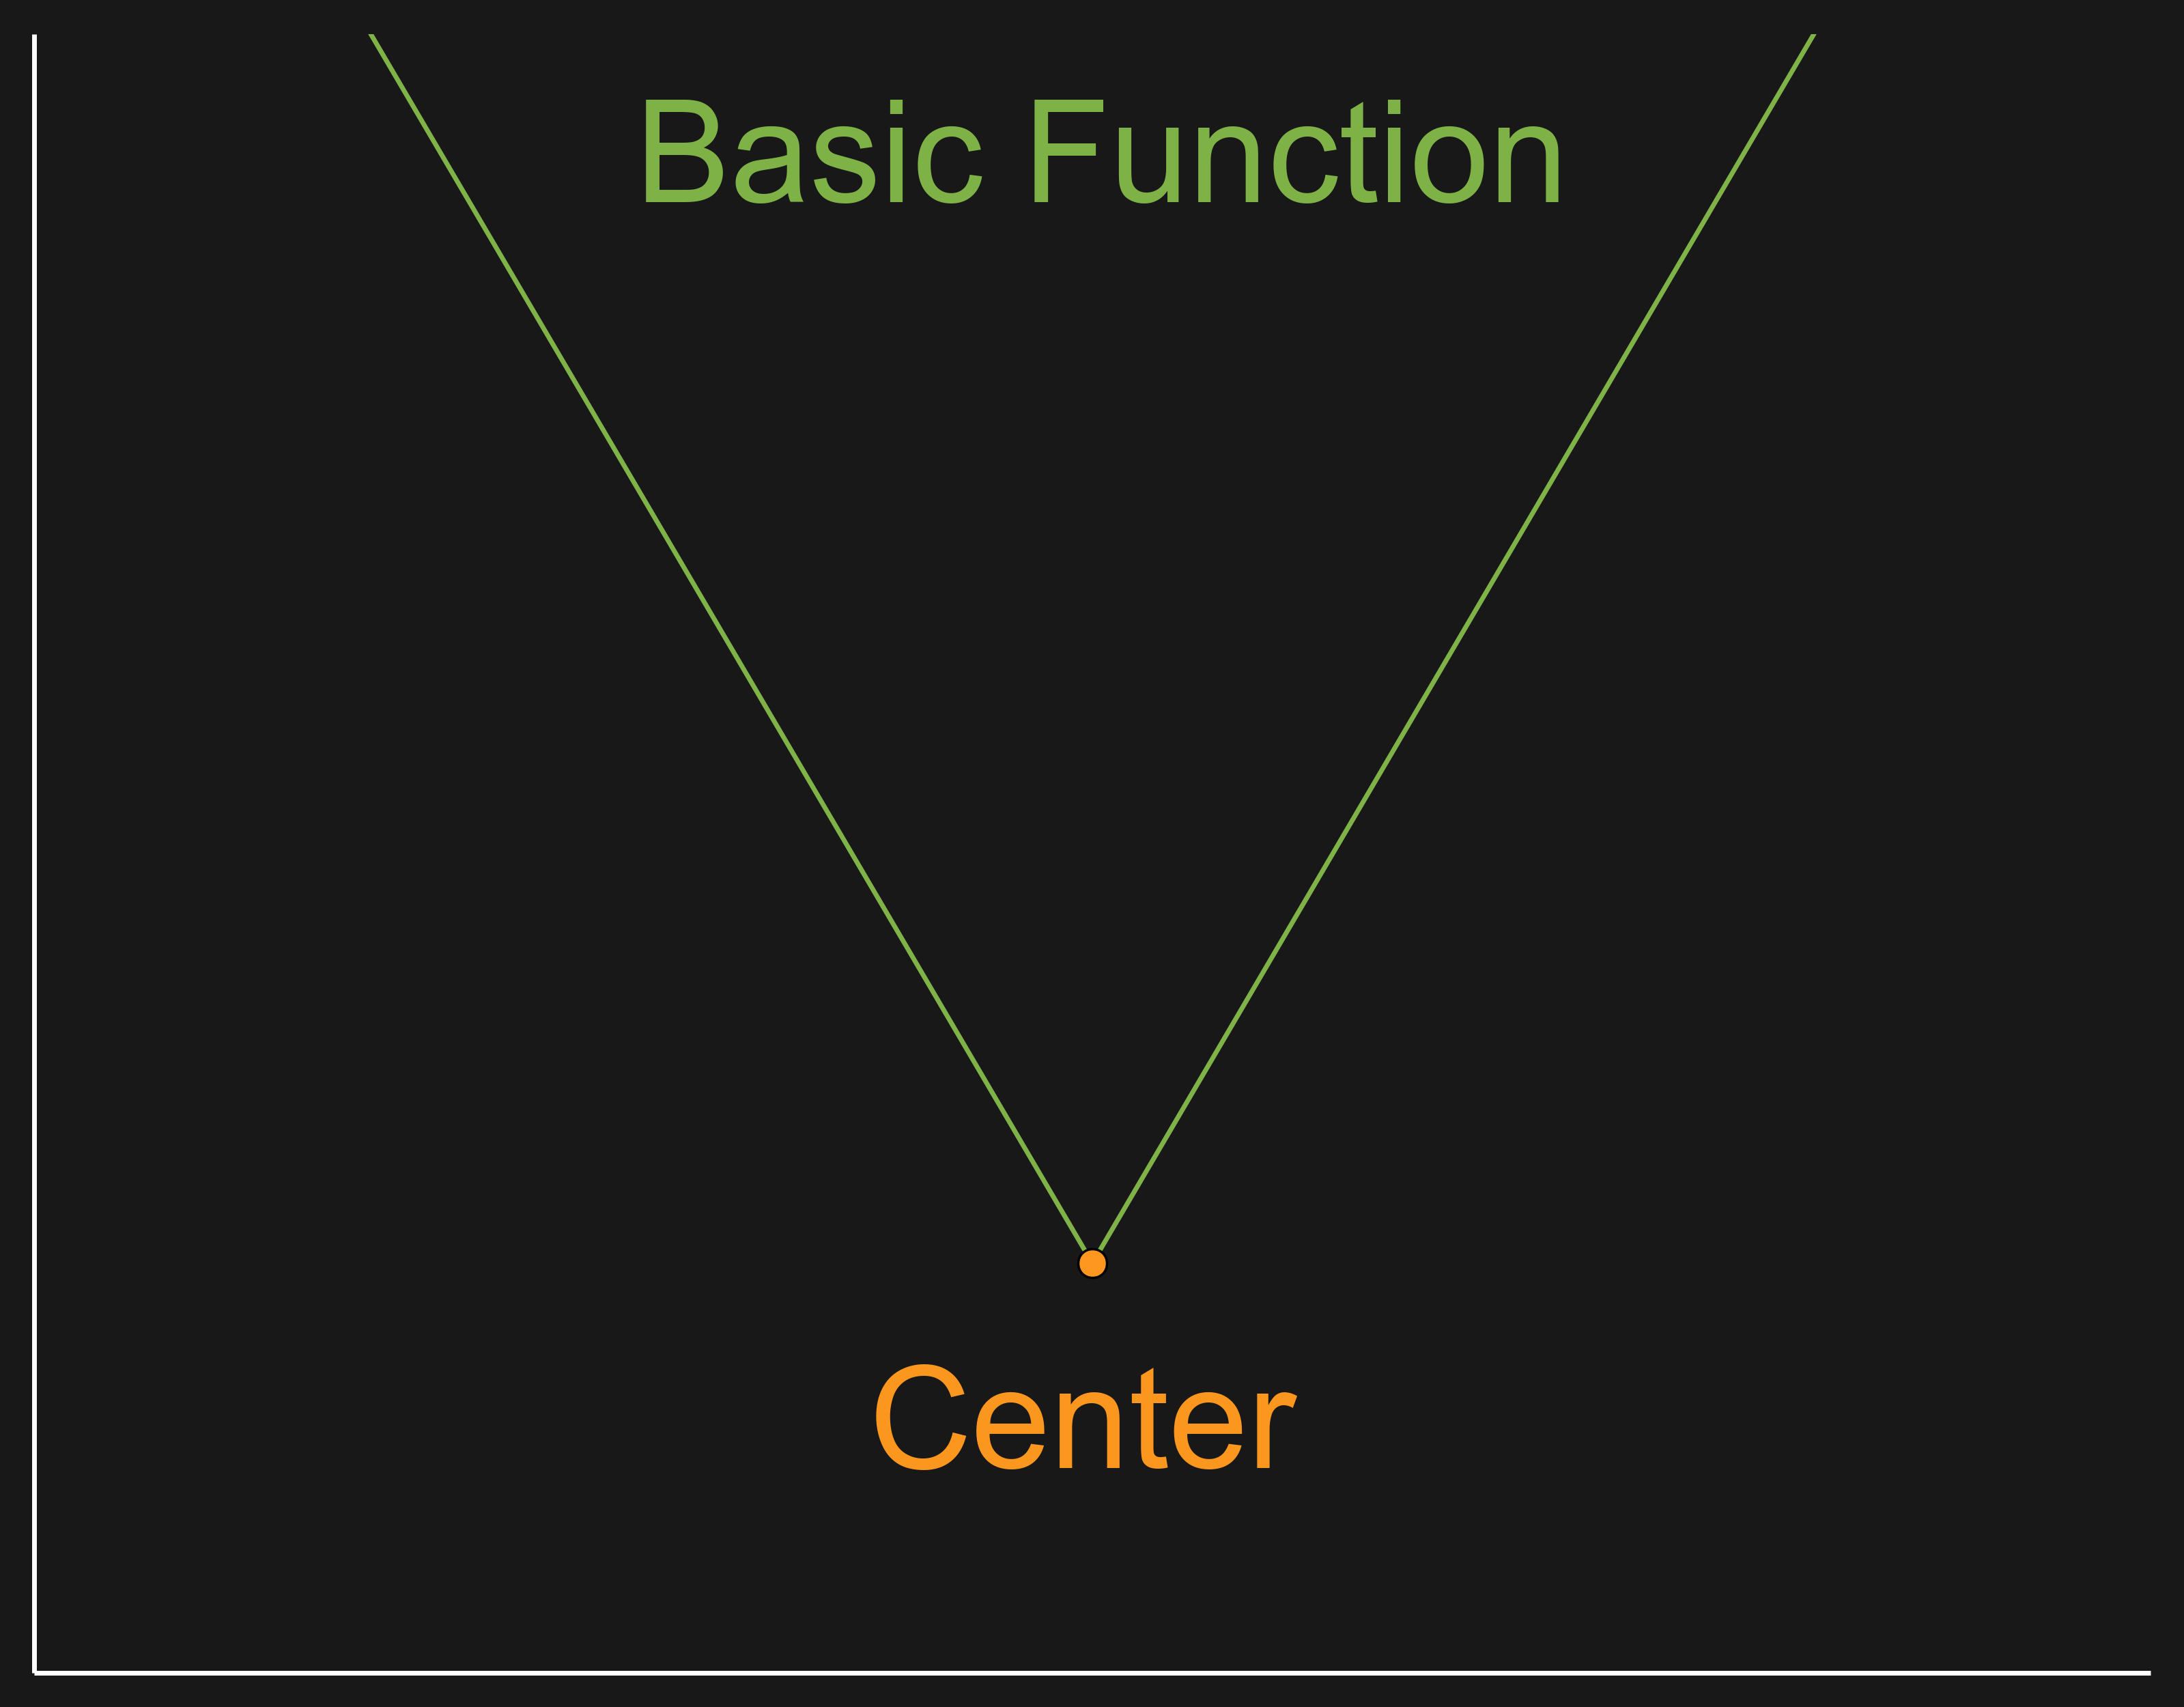
\includegraphics[width=0.7\textwidth, keepaspectratio]{fig4.png}
\end{figure}

\note{Change to || ||
Comment on Radial Symmetry}
\end{frame}

\begin{frame}{Basis Functions Depending on Data}
First, consider what we call the \subt{basic function}\\
\begin{equation*}
\psi(x)=|x|
\end{equation*}

To produce our set of basis functions, we take \subt{translates} of the basic function.

\begin{align*}
&\psi_i(x)=||x-x_i|| &i=1, \mathellipsis, N
\end{align*}

So each basis function, $\psi_i(x)$, is our basic function shifted so that the \subt{center} or \subt{knot} is positioned on a data site, $x_i$.
\bigskip

\subt{Note:} It's possible to have other choices of centers, but in most implementations the centers coincide with data sites.

\note{Change to || ||
Comment on Radial Symmetry}
\end{frame}

\begin{frame}{Basis Functions Depending on Data}
Each basis function, \textcolor{green}{$\psi_i(x)$}, is our basic function shifted so that the \textcolor{orange}{center} is positioned on a data site, \textcolor{orange}{$x_i$}.

\begin{align*}
&\psi_i(x)=||x-x_i||  &i=1, \mathellipsis, N
\end{align*}


\begin{figure}
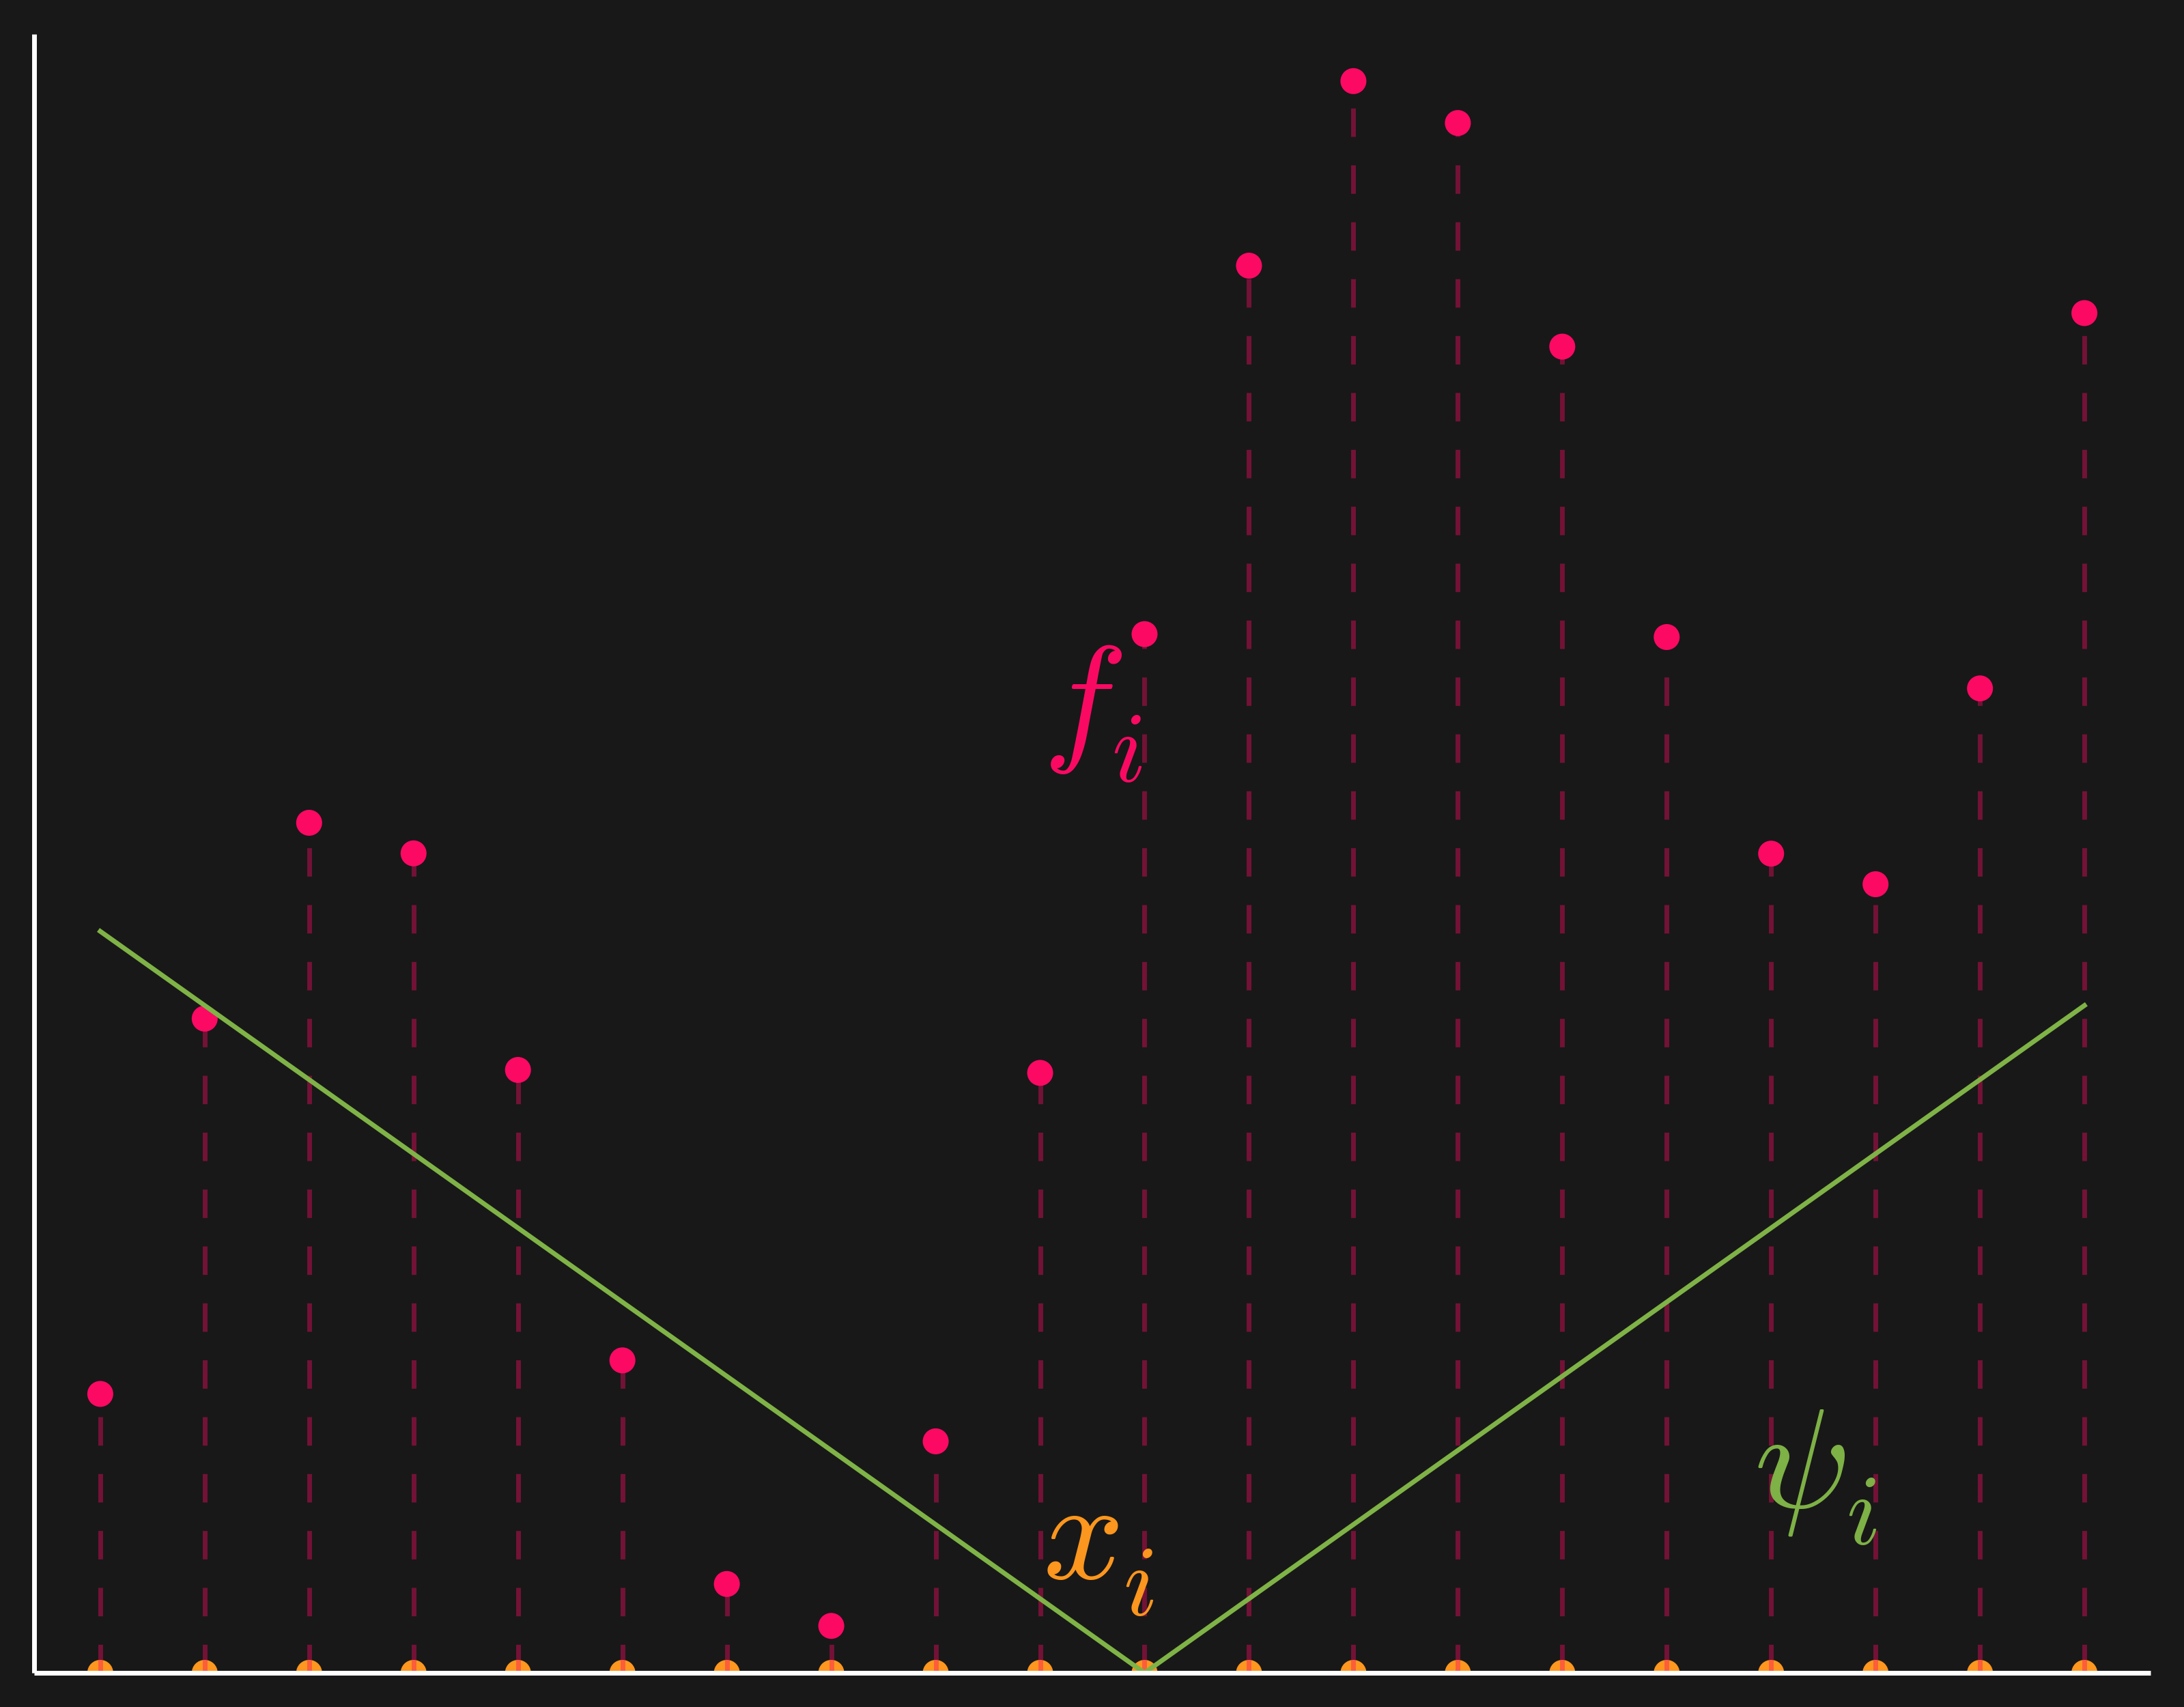
\includegraphics[width=0.65\textwidth, keepaspectratio]{fig5.png}
\end{figure}


\note{Change to || ||
Comment on Radial Symmetry}
\end{frame}

\begin{frame}{Radial Basis Functions}

\begin{align*}
&\psi_i(x)=||x-x_i||     & i=1, \mathellipsis, N
\end{align*}

Notice that $\psi_i(x)$ are radially symmetric about their centers, for this reason we call these functions \subt{Radial Basis Functions (RBF)}.
\bigskip

Since the basis functions only depend on distance, the interpolation matrix becomes
\begin{equation*}
A=
\begin{bmatrix}
||x_1-x_1|| & ||x_1-x_2|| & \cdots & ||x_1-x_N||\\
||x_2-x_1|| & ||x_2-x_2||& \cdots & ||x_2-x_N||\\
\vdots & \vdots & \ddots & \vdots\\
||x_N-x_1|| & ||x_N-x_2||& \cdots & ||x_N-x_N||
\end{bmatrix}
\end{equation*}
called a \subt{distance matrix}.

\note{}
\end{frame}

\begin{frame}{The Distance Matrix}
Distance matrices, with Euclidean distances, for distinct points in $\mathbb{R}^s$ are always non-singular.
\bigskip

This means that our interpolation problem

\begin{equation*}
\begin{bmatrix}
||x_1-x_1|| & ||x_1-x_2|| & \cdots & ||x_1-x_N||\\
||x_2-x_1|| & ||x_2-x_2||& \cdots & ||x_2-x_N||\\
\vdots & \vdots & \ddots & \vdots\\
||x_N-x_1|| & ||x_N-x_2||& \cdots & ||x_N-x_N||
\end{bmatrix}
\begin{bmatrix}
\lambda_1\\
\lambda_2\\
\vdots\\
\lambda_N
\end{bmatrix}
=
\begin{bmatrix}
f_1\\
f_2\\
\vdots\\
f_N
\end{bmatrix}
\end{equation*}
is well-posed!
\bigskip

Our interpolant becomes 
\subt{$s(x)=\sum_{i=1}^N \lambda_i ||x-x_i|| $}

\note{}
\end{frame}

\begin{frame}{Building a Better Basic Function}
Basic function
\begin{equation*}
\psi_i(x)=||x-x_i||
\end{equation*}
has a discontinuity in its first derivative at $x_i$.

\begin{figure}
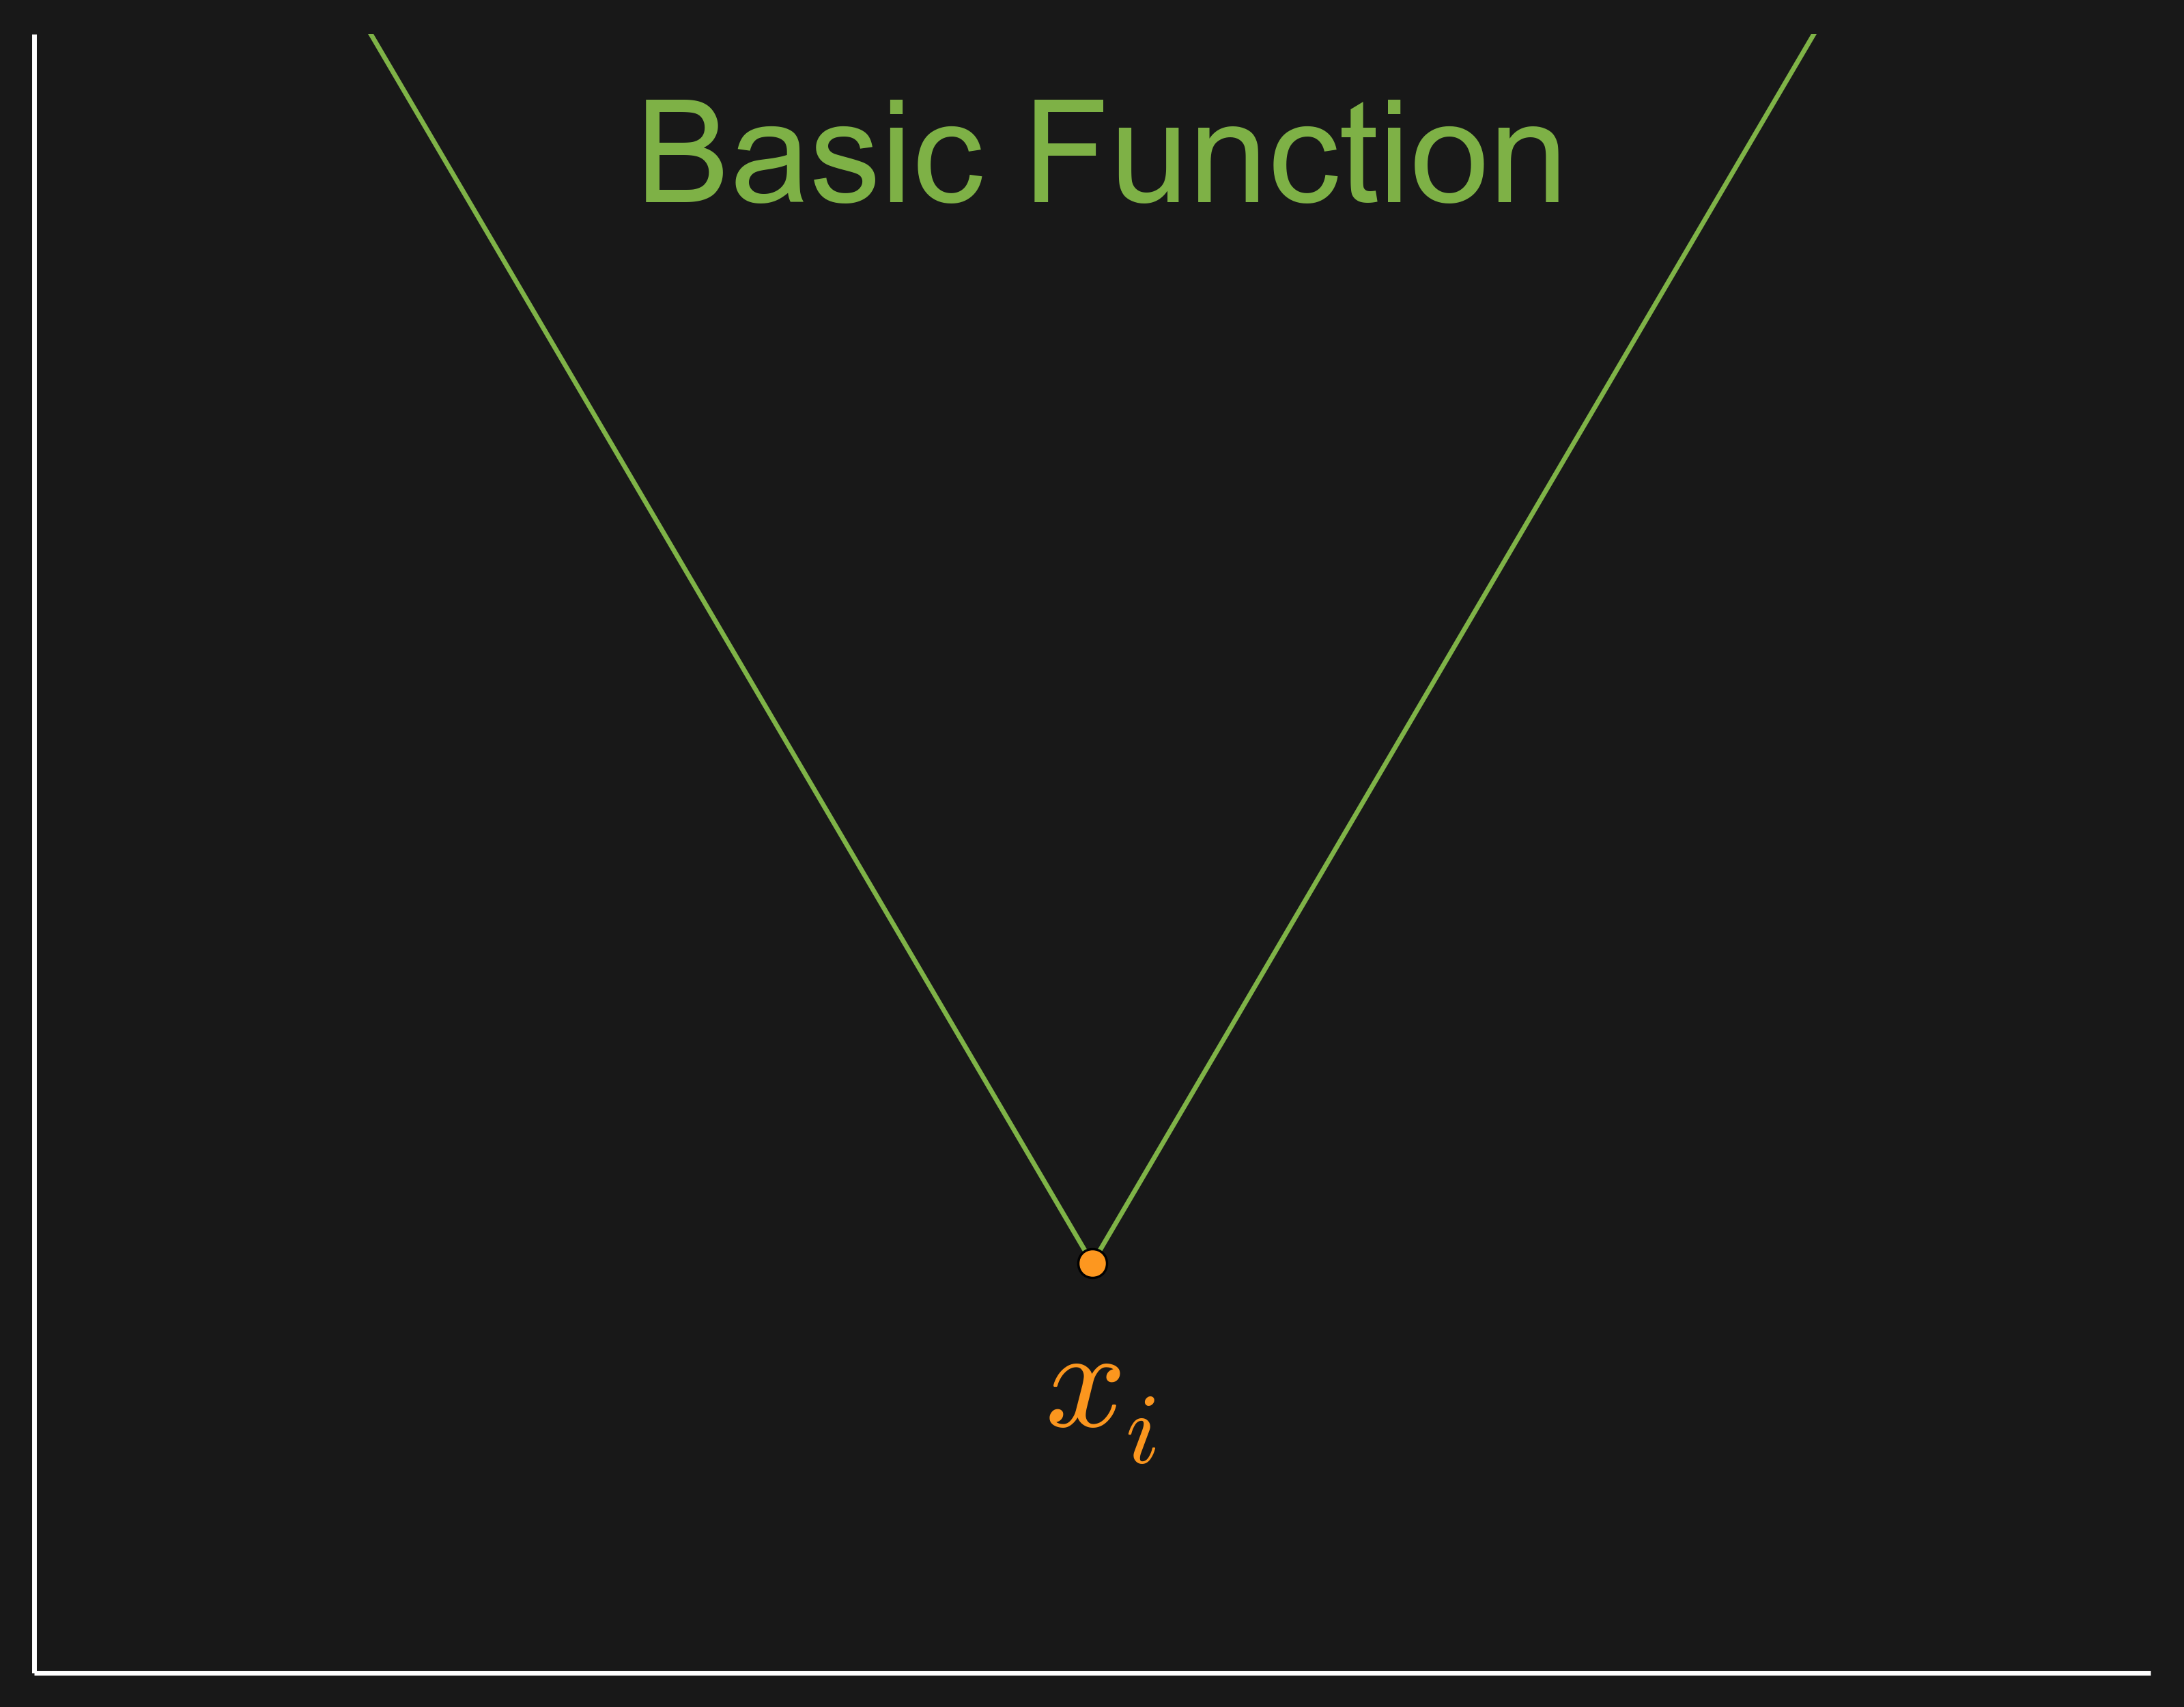
\includegraphics[width=0.5\textwidth, keepaspectratio]{fig6.png}
\end{figure}
This causes the interpolant to have a discontinuous first derivative at each data site. 

Obviously not ideal.

\note{}
\end{frame}

\begin{frame}{Building a Better Basic Function}

In 1968, R.L. Hardy showed that we can remedy this problem by changing our basic function so it's $C^\infty$.

\subt{Hardy's Multiquadrc Kernel}
\begin{align*}
&\psi(x)=\sqrt{c^2 + x^2} &\text{where   } &c \neq 0.
\end{align*}


\begin{figure}
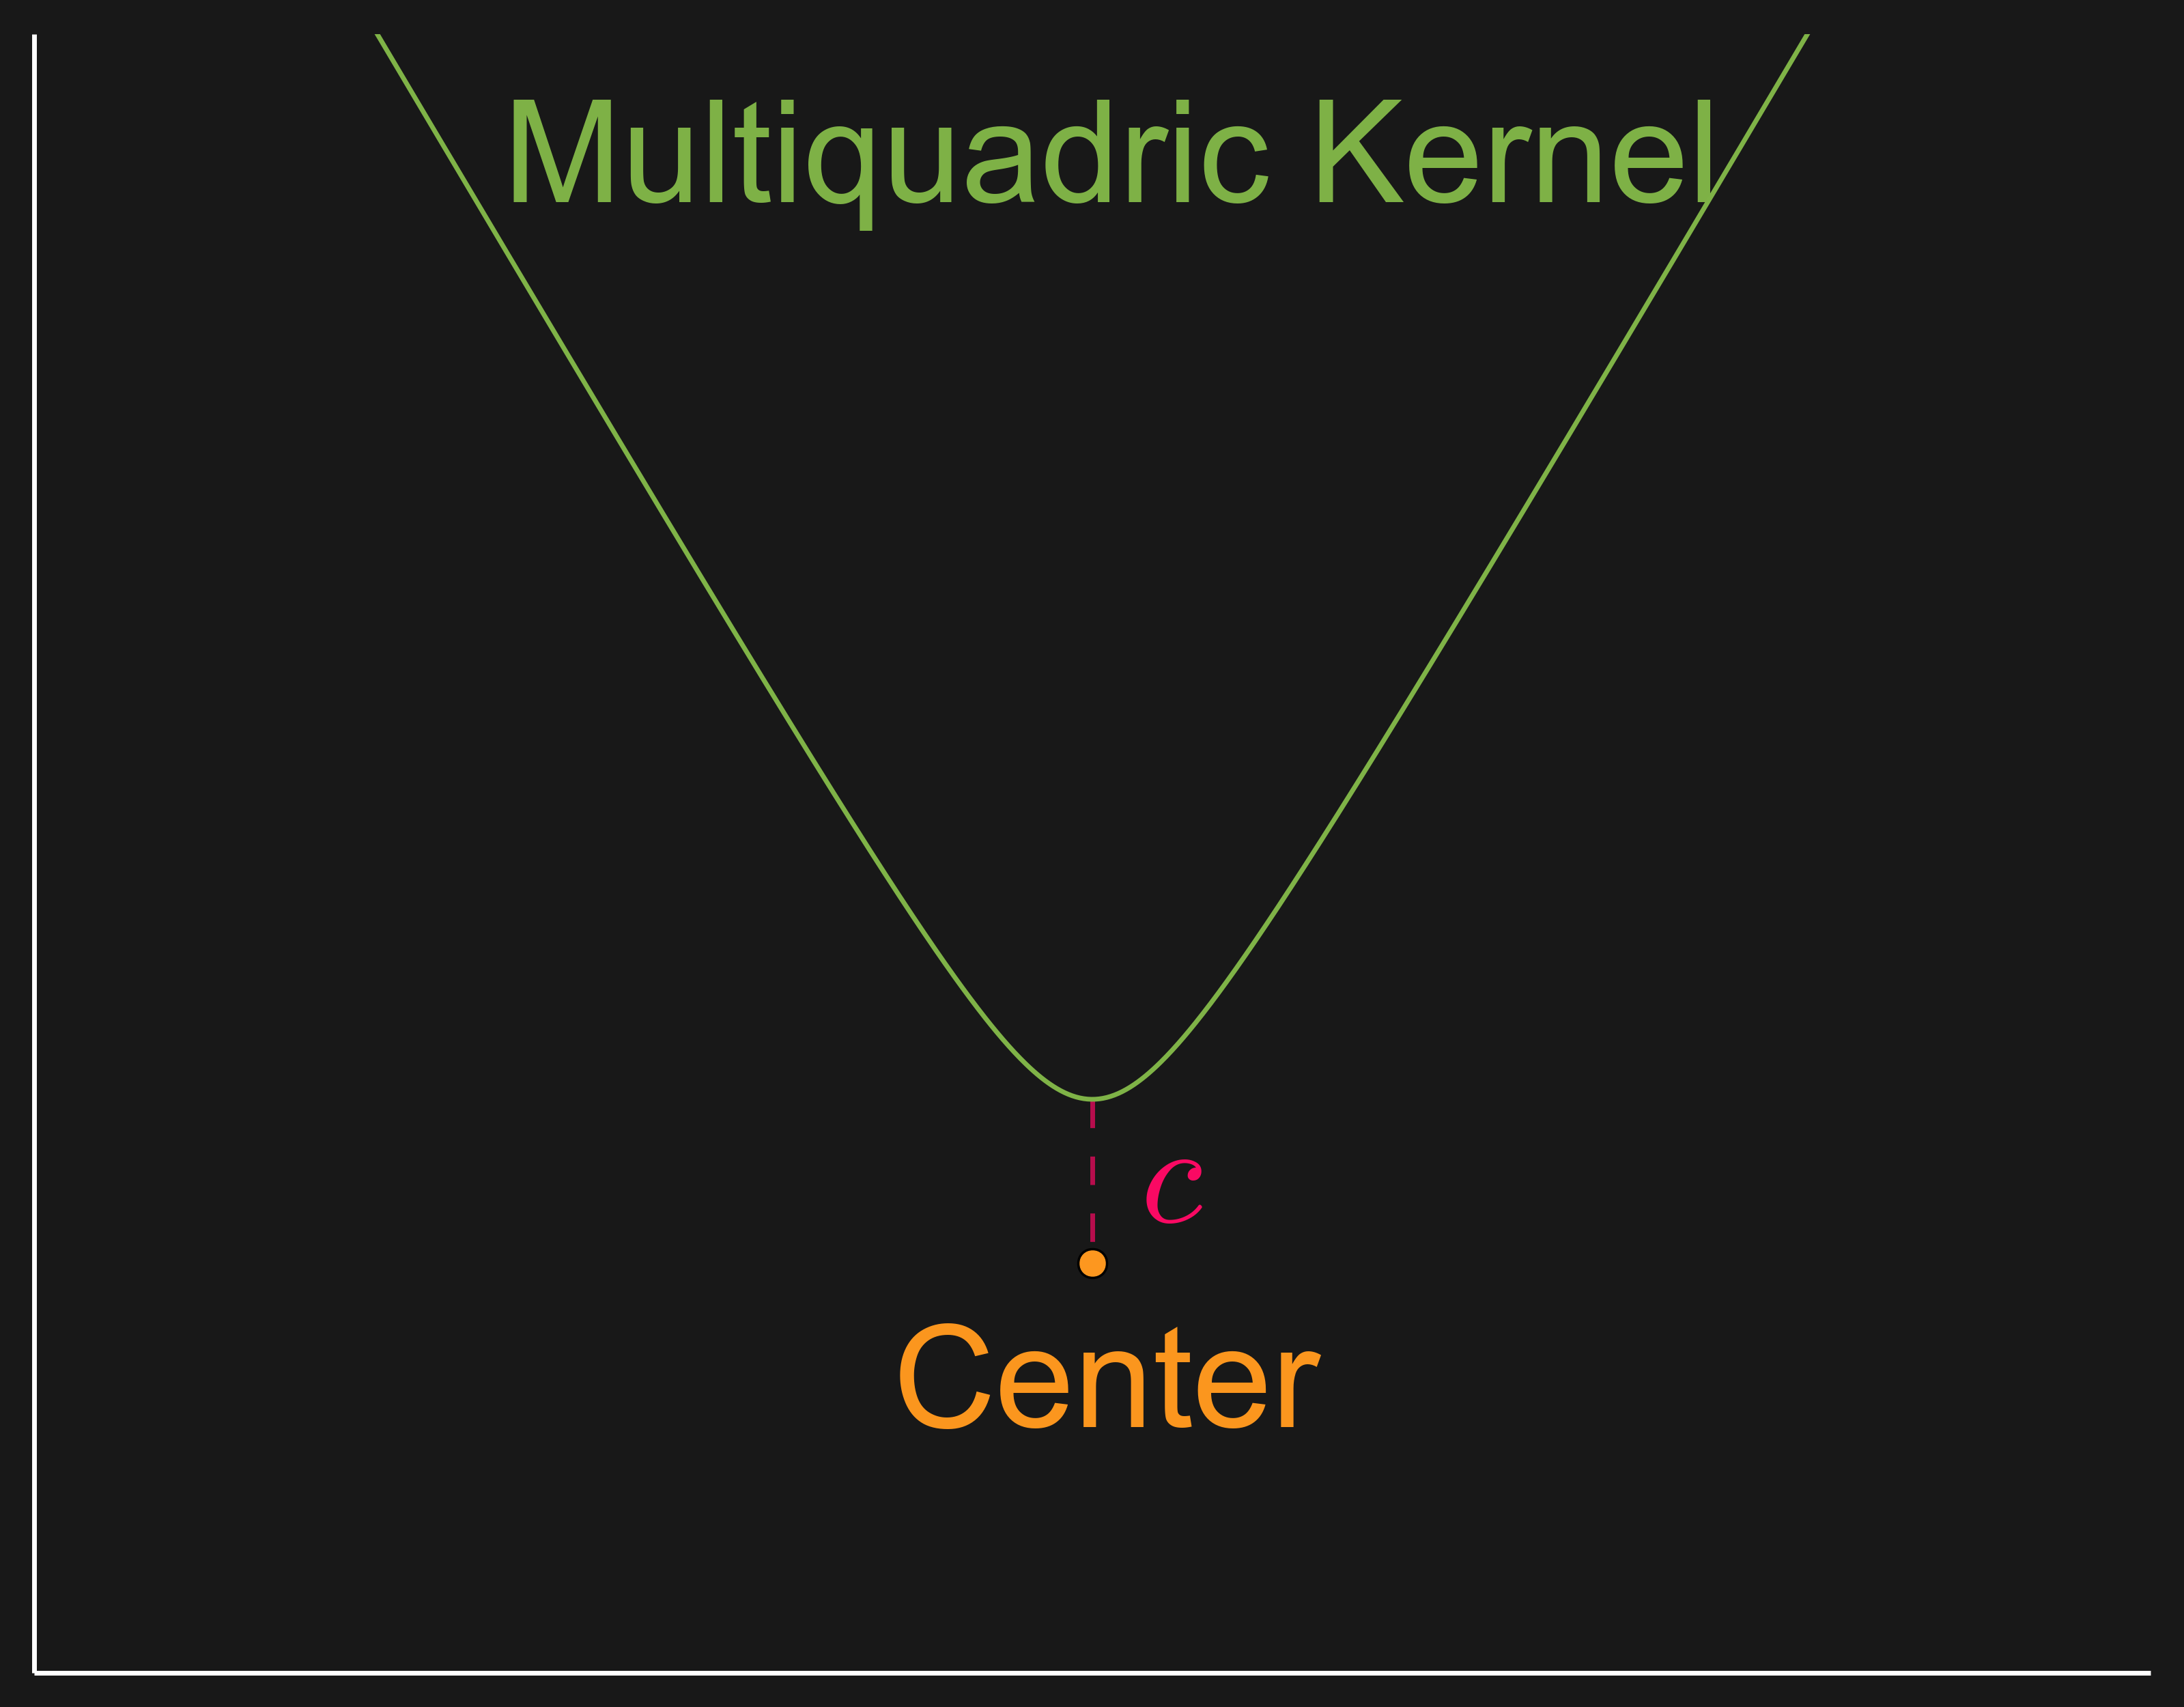
\includegraphics[width=0.5\textwidth, keepaspectratio]{fig7.png}
\end{figure}

\subt{Note:} \textcolor{pink}{$c$} is called the shape parameter. The case when $c=0$ is 
 the previous basic function.

\note{}
\end{frame}

\begin{frame}{Radial Basis Kernels}
As before, we can generate our basis functions by translating Hardy's basic function to center on our data sites.
\begin{equation*}
\psi_i(x)=\sqrt{c^2 + (||x-x_i||)^2}
\end{equation*}
\begin{figure}
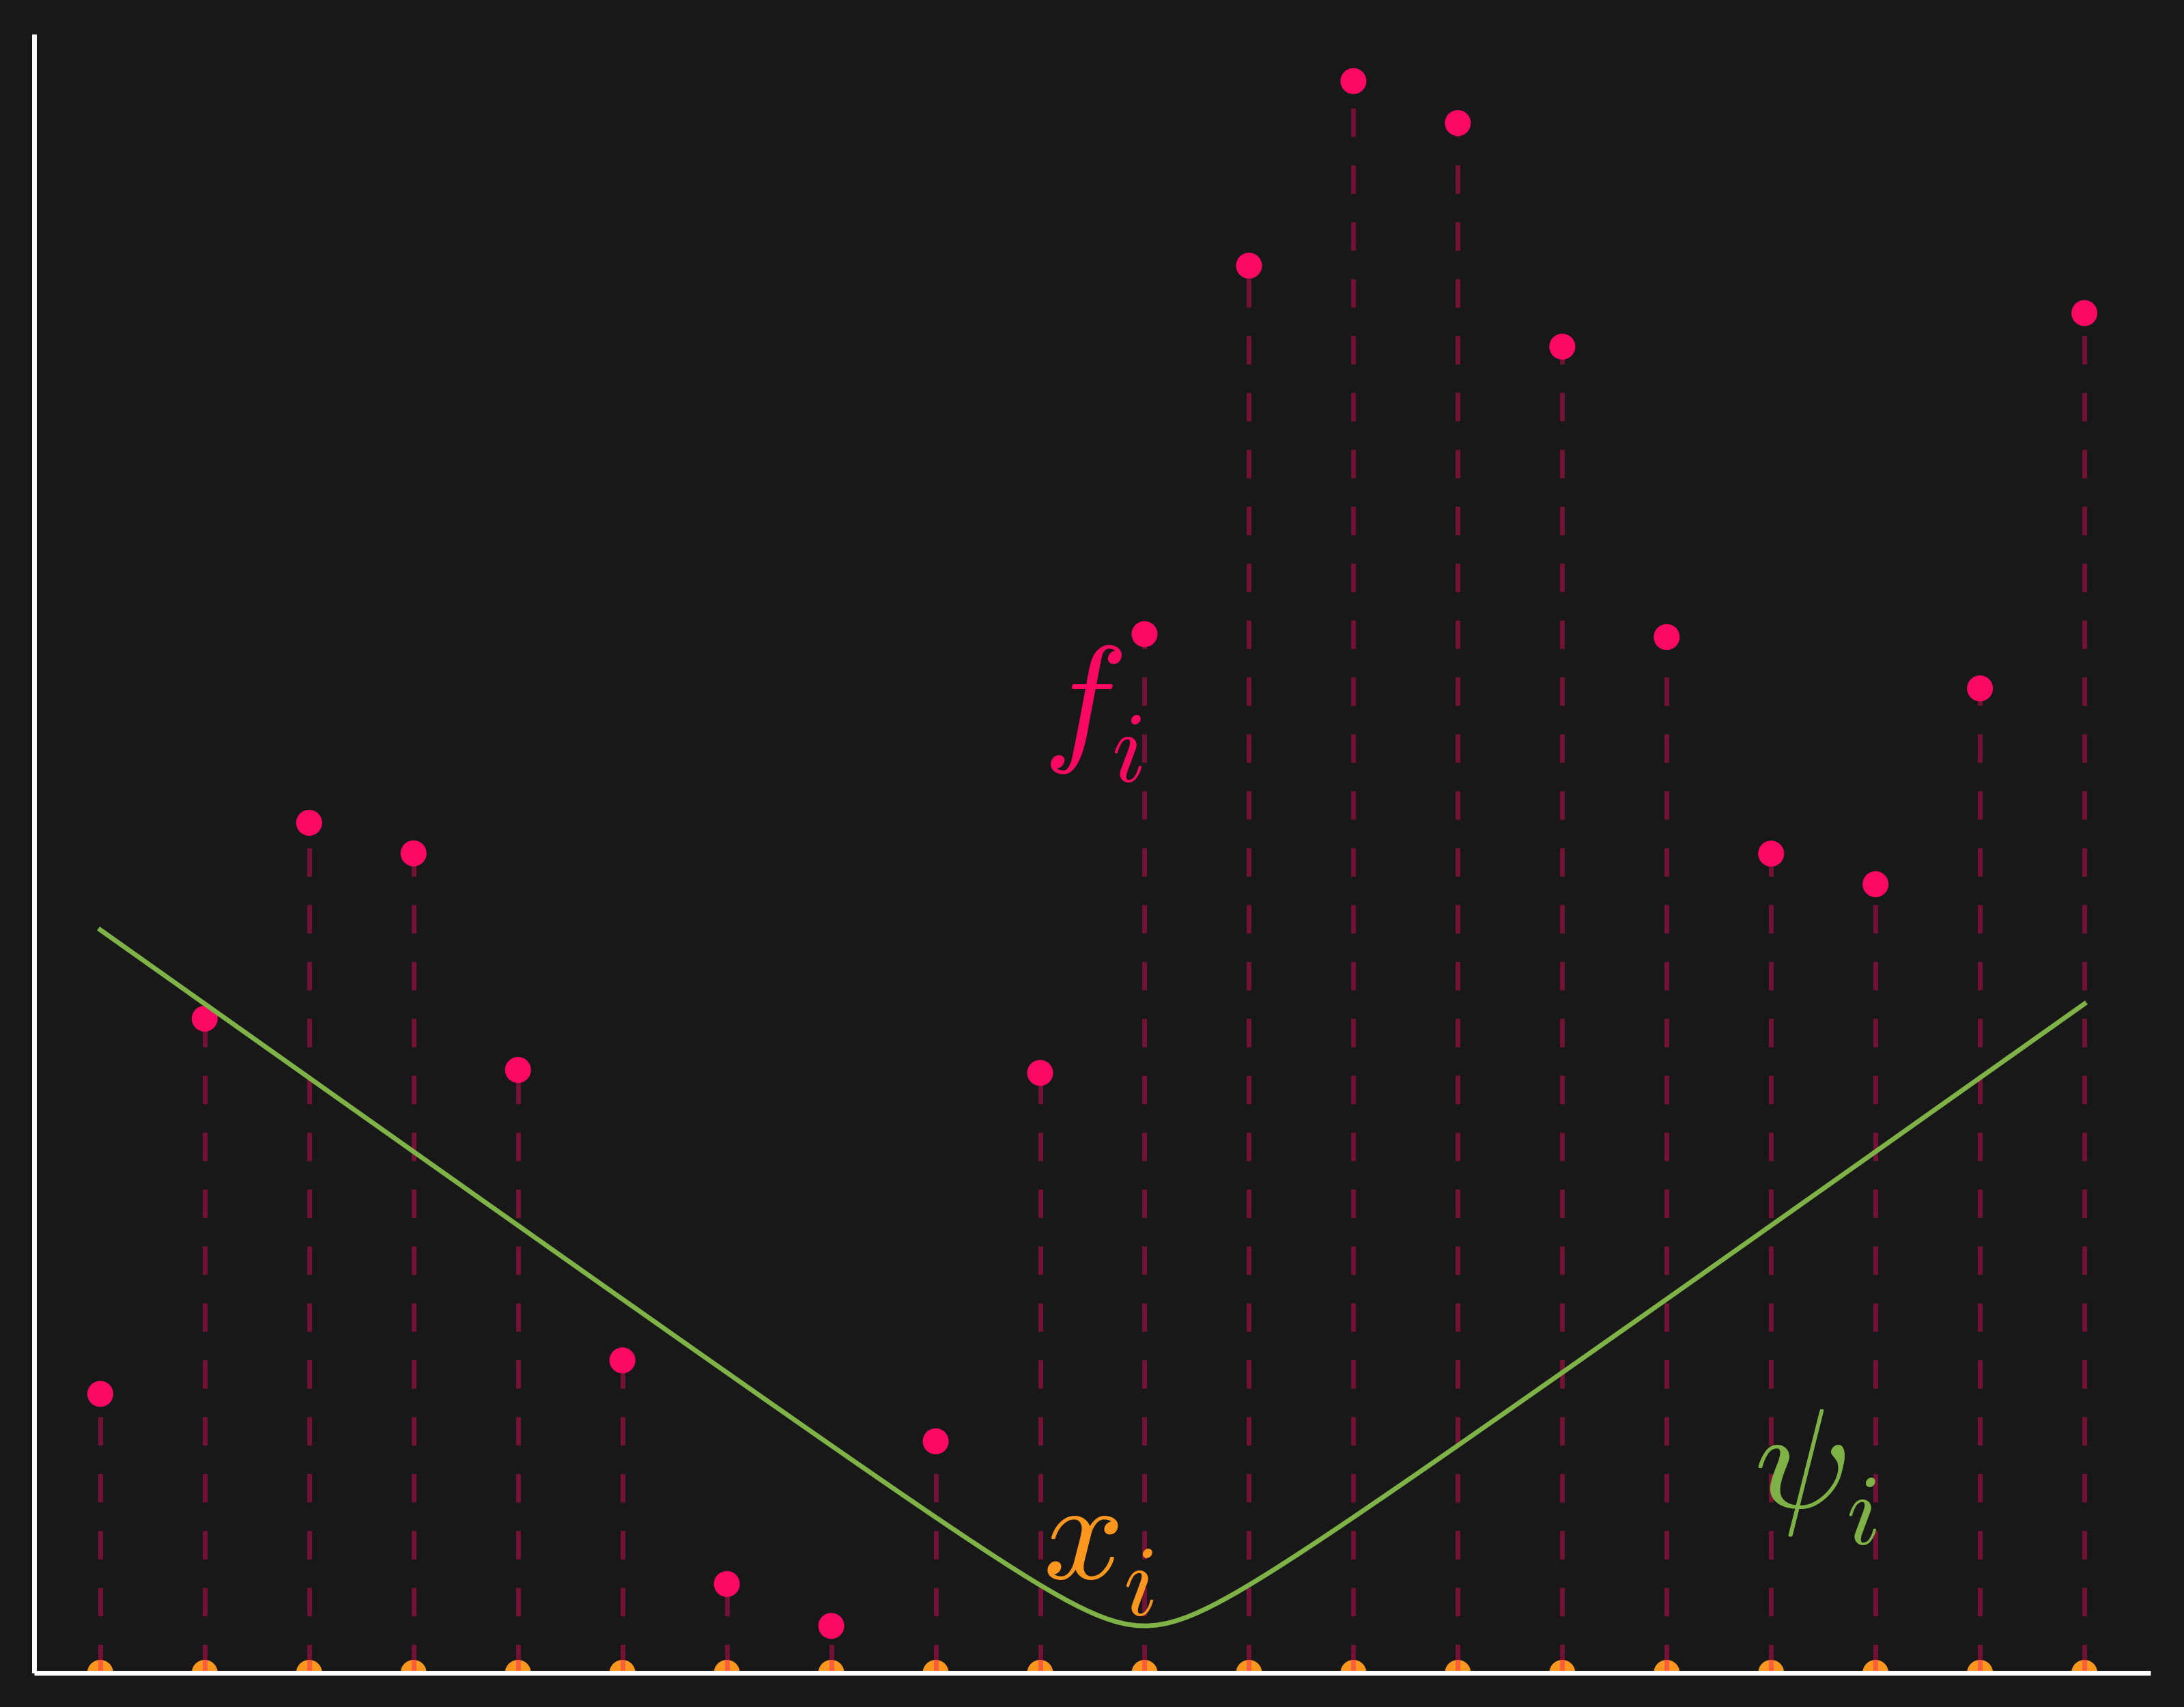
\includegraphics[width=0.7\textwidth, keepaspectratio]{fig8.png}
\end{figure}

\note{}
\end{frame}

\begin{frame}{Radial Basis Kernels}
Hardy's Multiquadric function is still \subt{radially symmetric} about its center


\begin{figure}
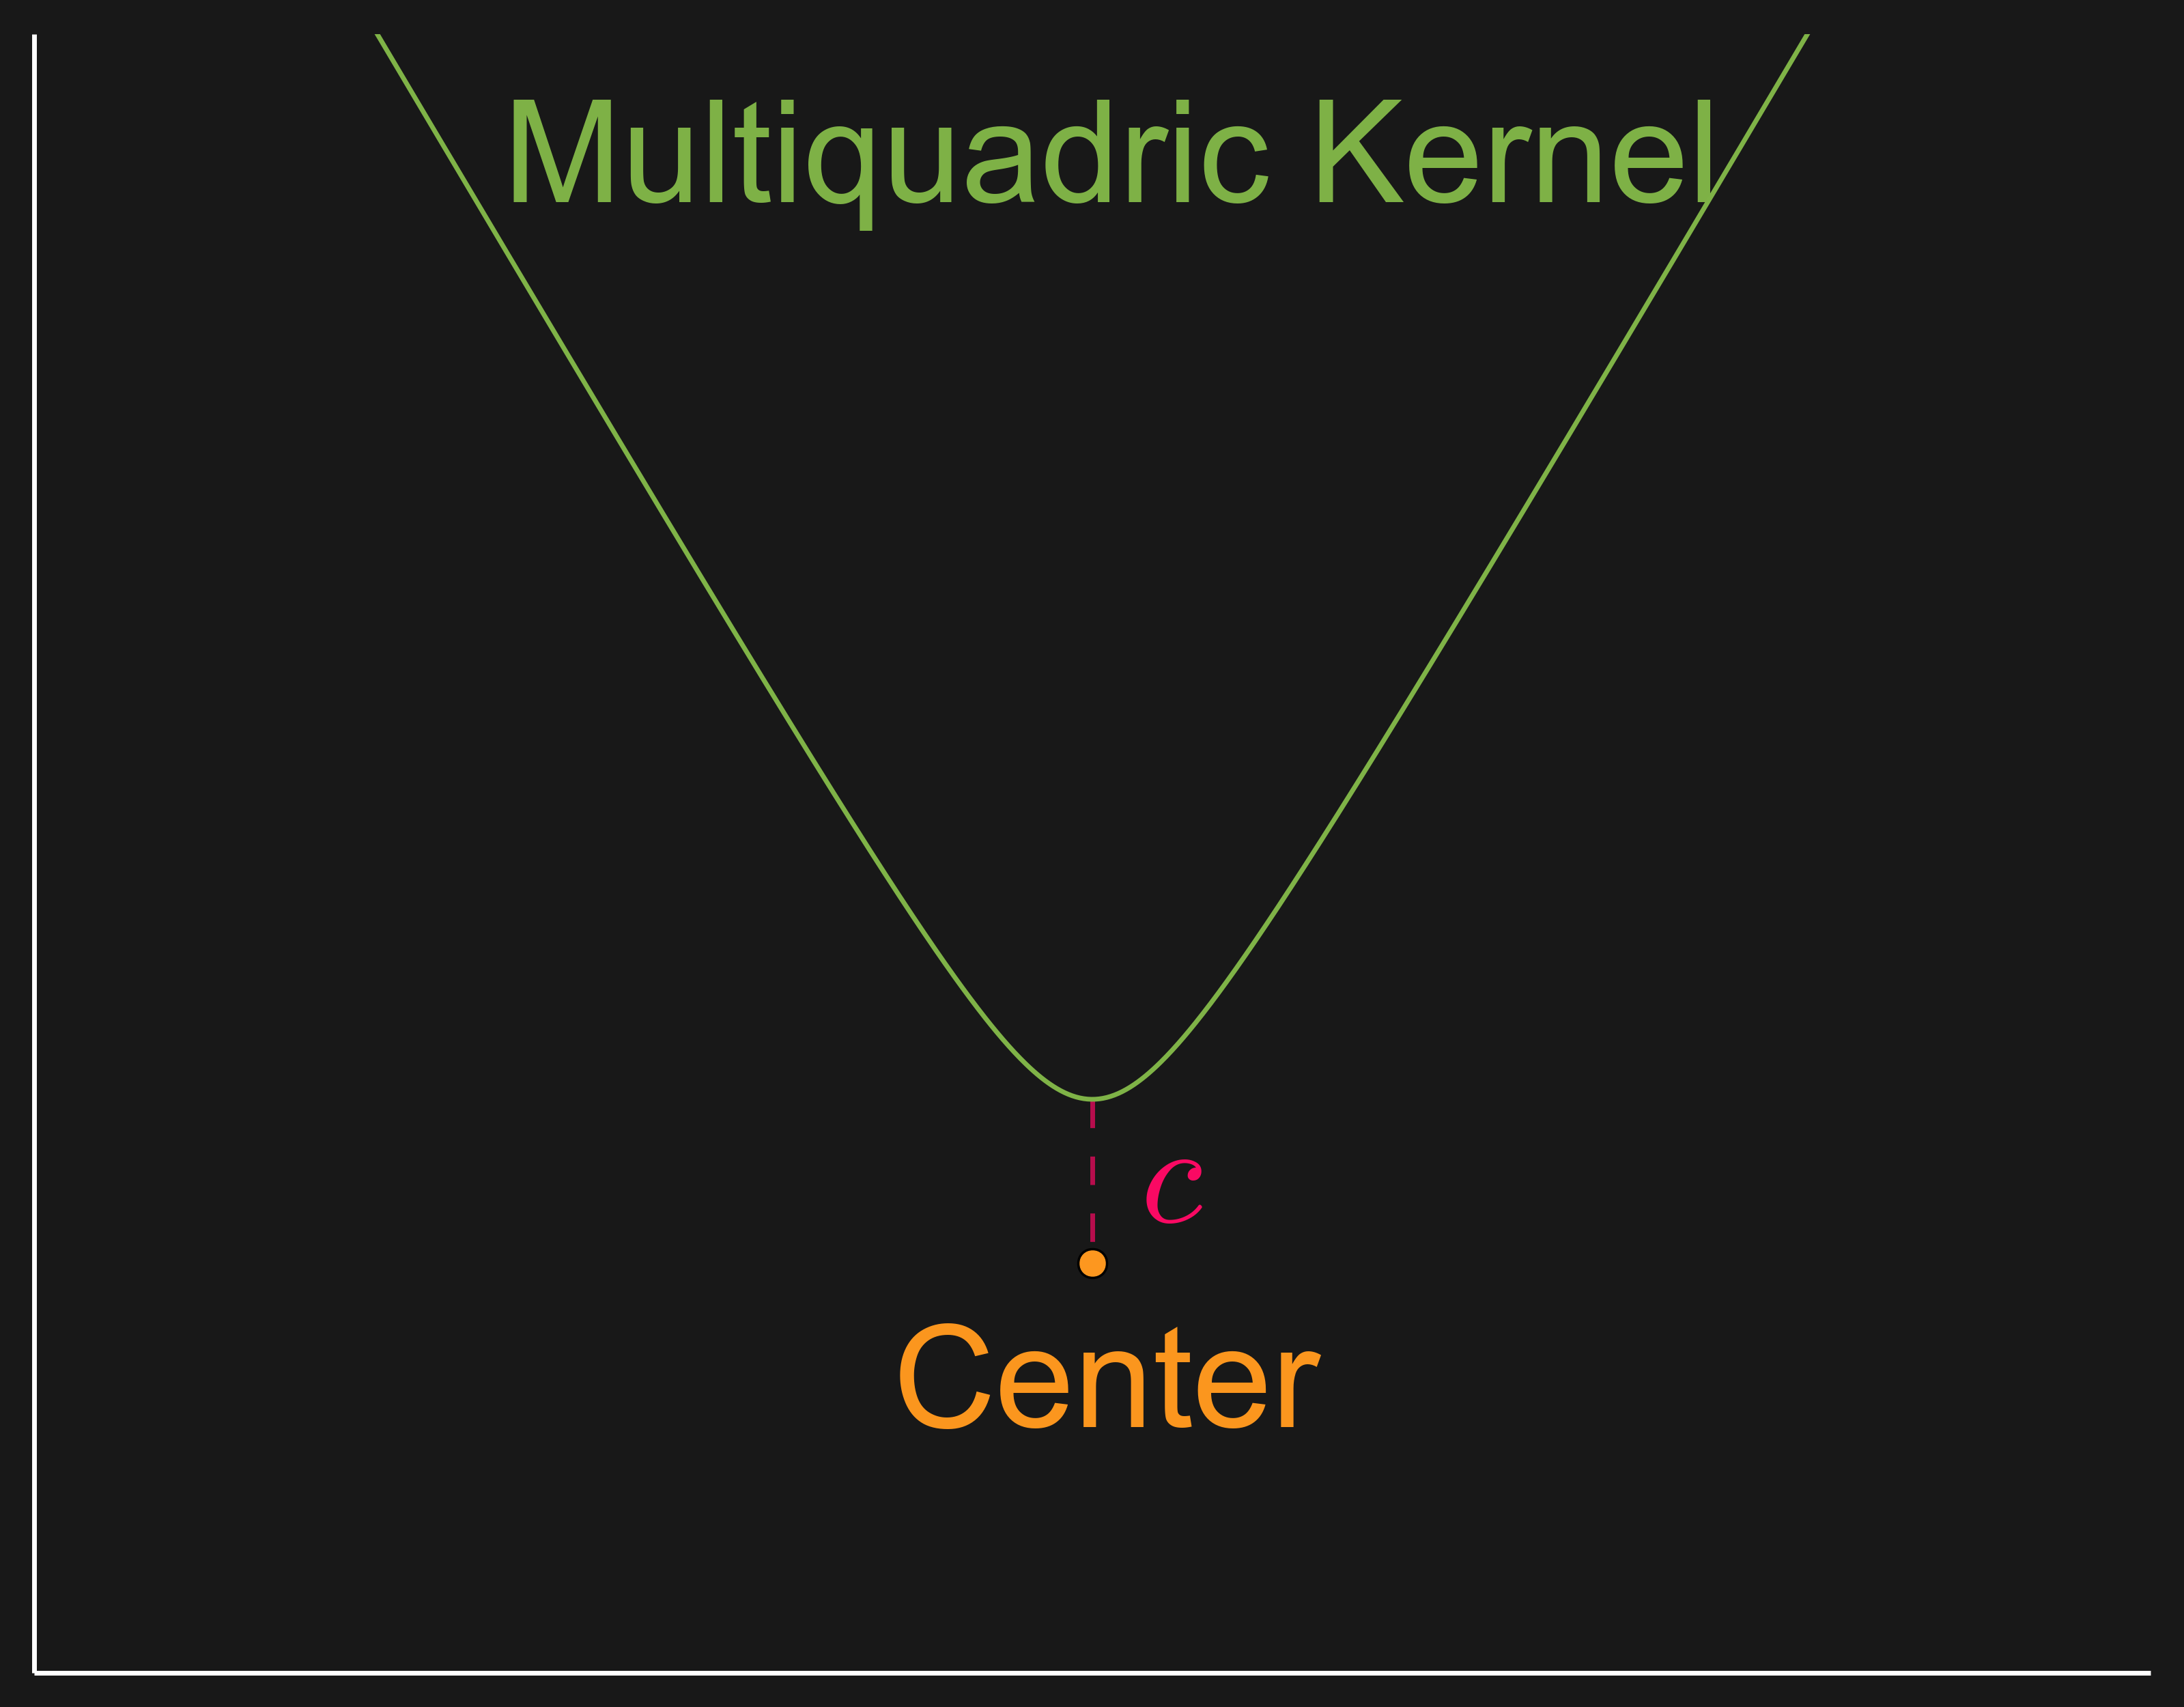
\includegraphics[width=0.3\textwidth, keepaspectratio]{fig7.png}
\end{figure}
we this function a Kernel. 

All Kernels are functions only of distance from center, and can be written generally as $\phi(||x-x_i||)$ or $\phi(r)$

\subt{The RBF Method}
\begin{align*}
&s(x)=\sum_{i=1}^N \lambda_i \phi(||x-x_i||)=\sum_{i=1}^N \lambda_i \phi(r) &r=||x-x_i||
\end{align*}

\note{}
\end{frame}

\begin{frame}{Radial Basis Kernels}


% \begin{table}
%   [ht] 
  \begin{tabular}
      {lll}  Common RBF Kernels  & $\phi(r)$\\
      \hline Multiquadric & $\sqrt{1+(\epsilon r)^2}$  & \parbox[c]{1em}{
      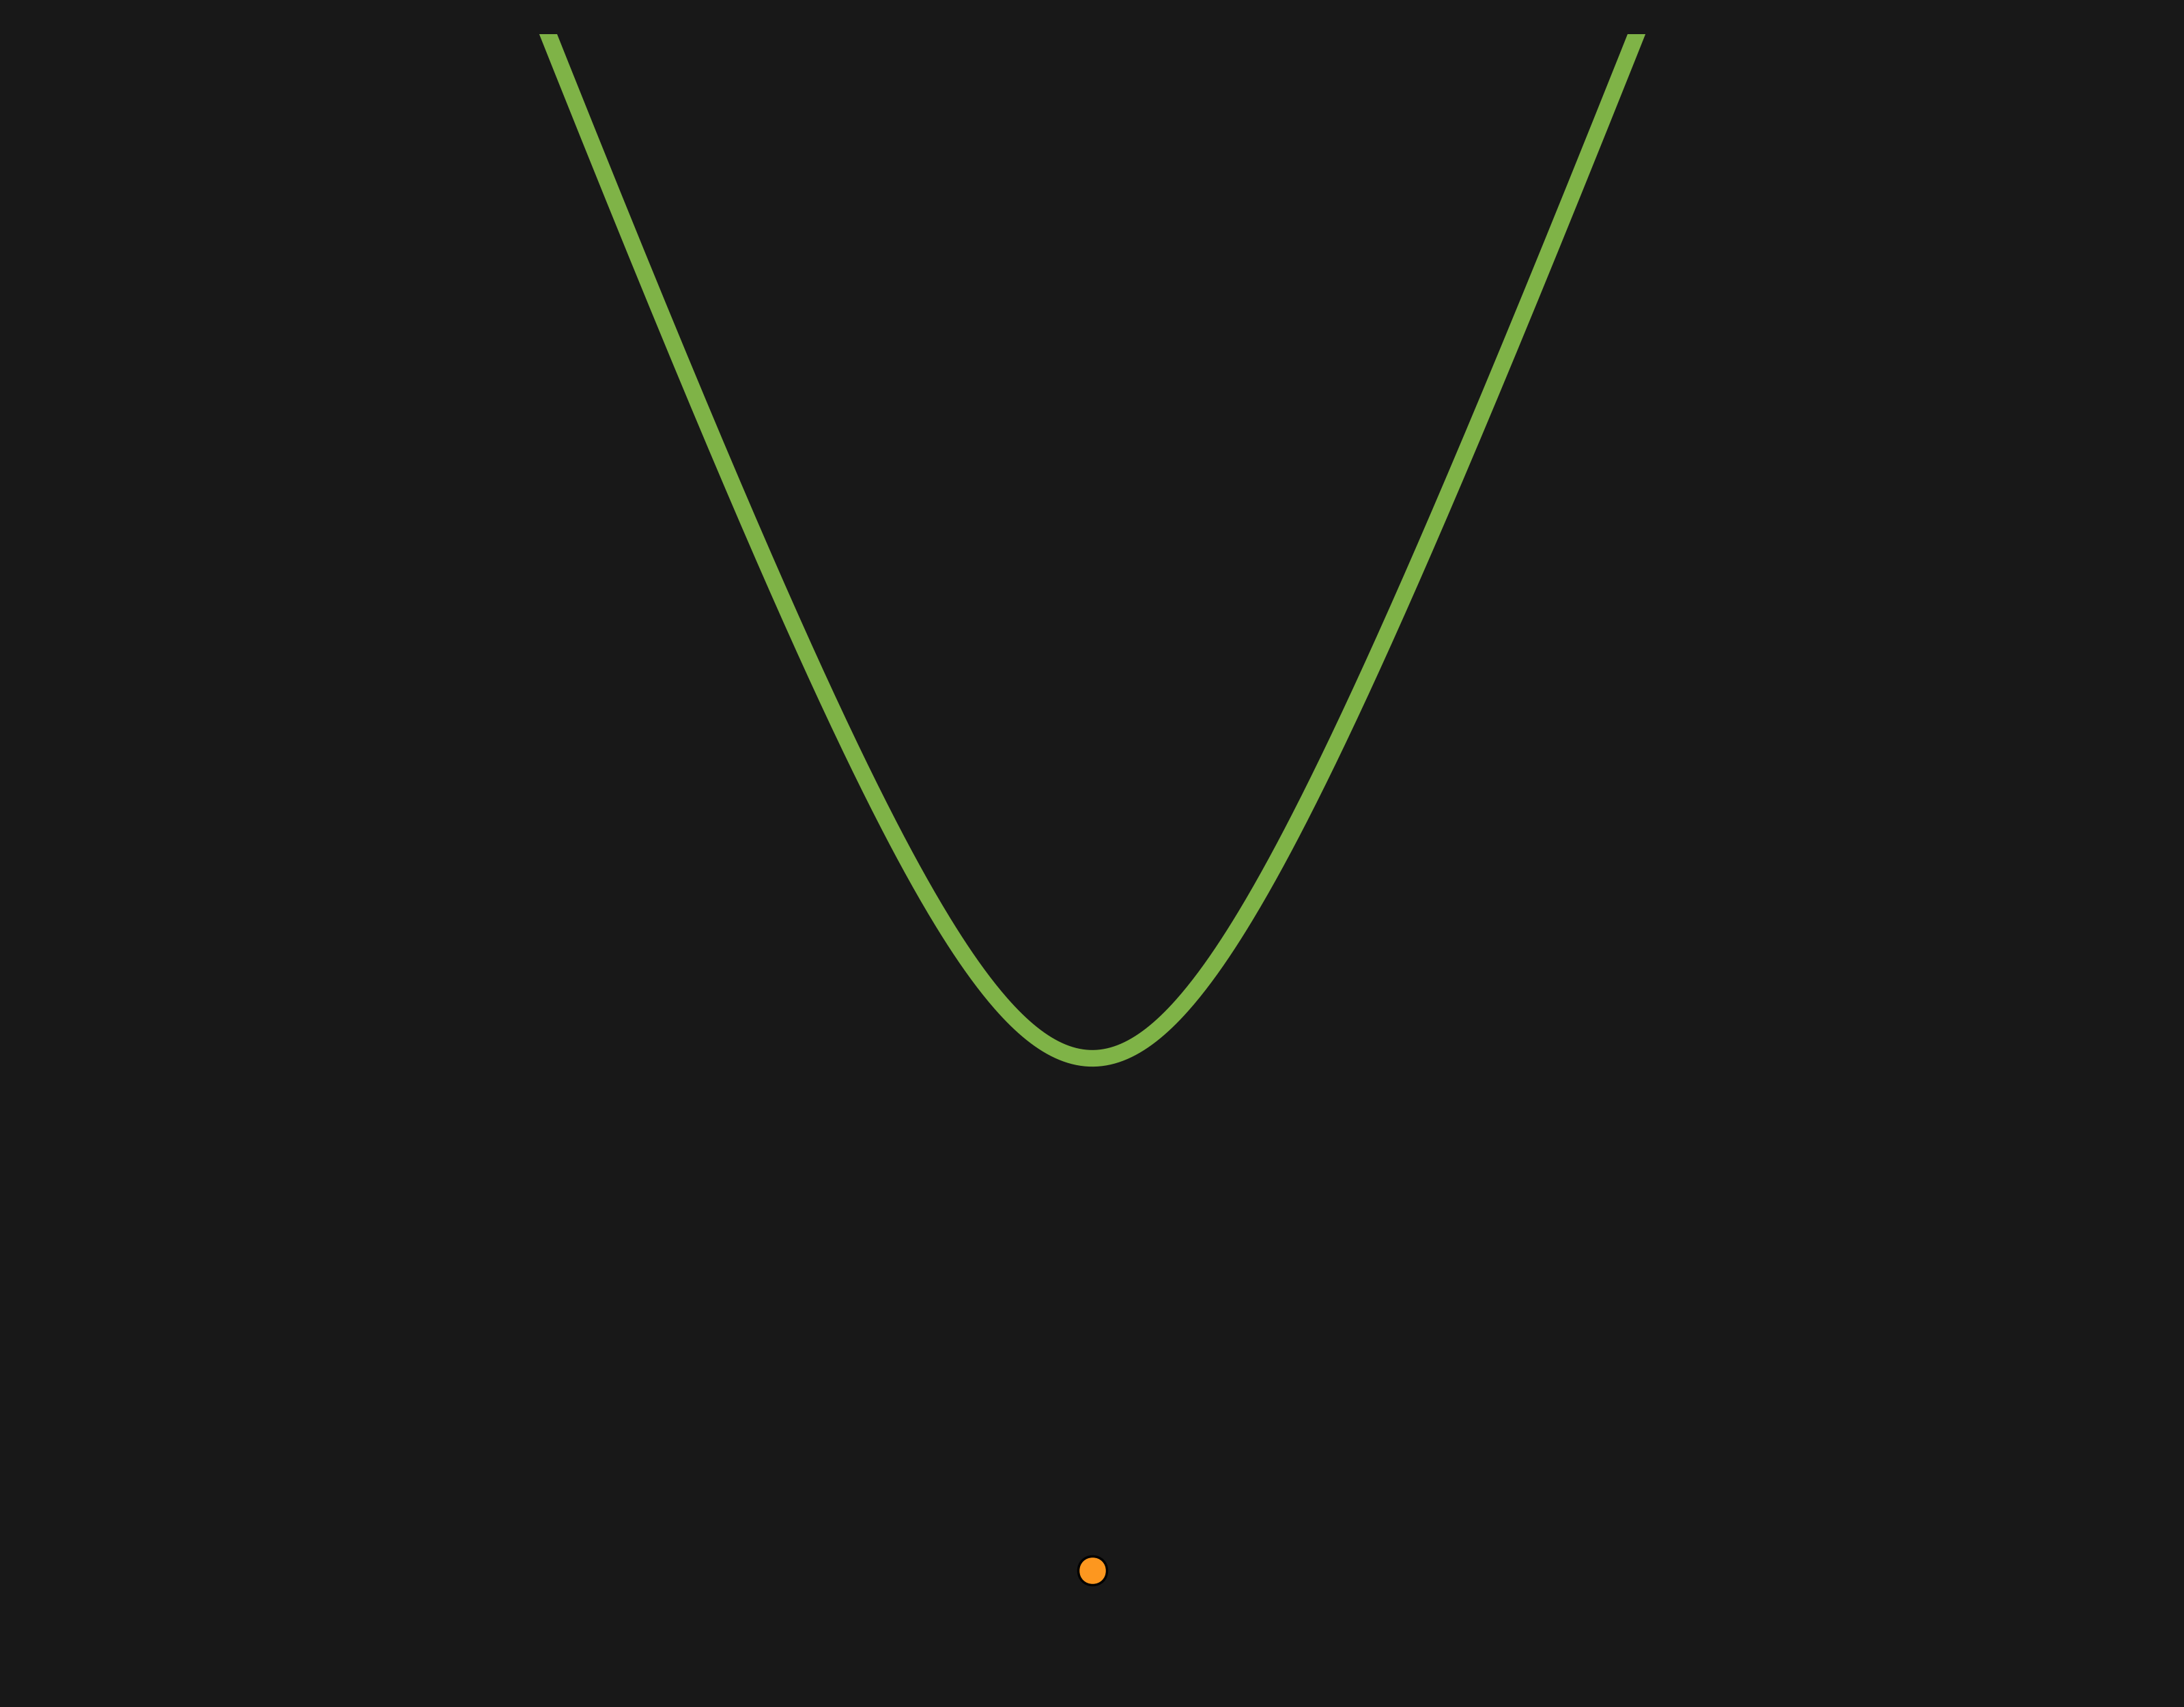
\includegraphics[width=0.2\textwidth]{multiquadric.png}} \\
      \hline Inverse Multiquadric & $\frac{1}{\sqrt{1+(\epsilon r)^2}}$  & \parbox[c]{1em}{
      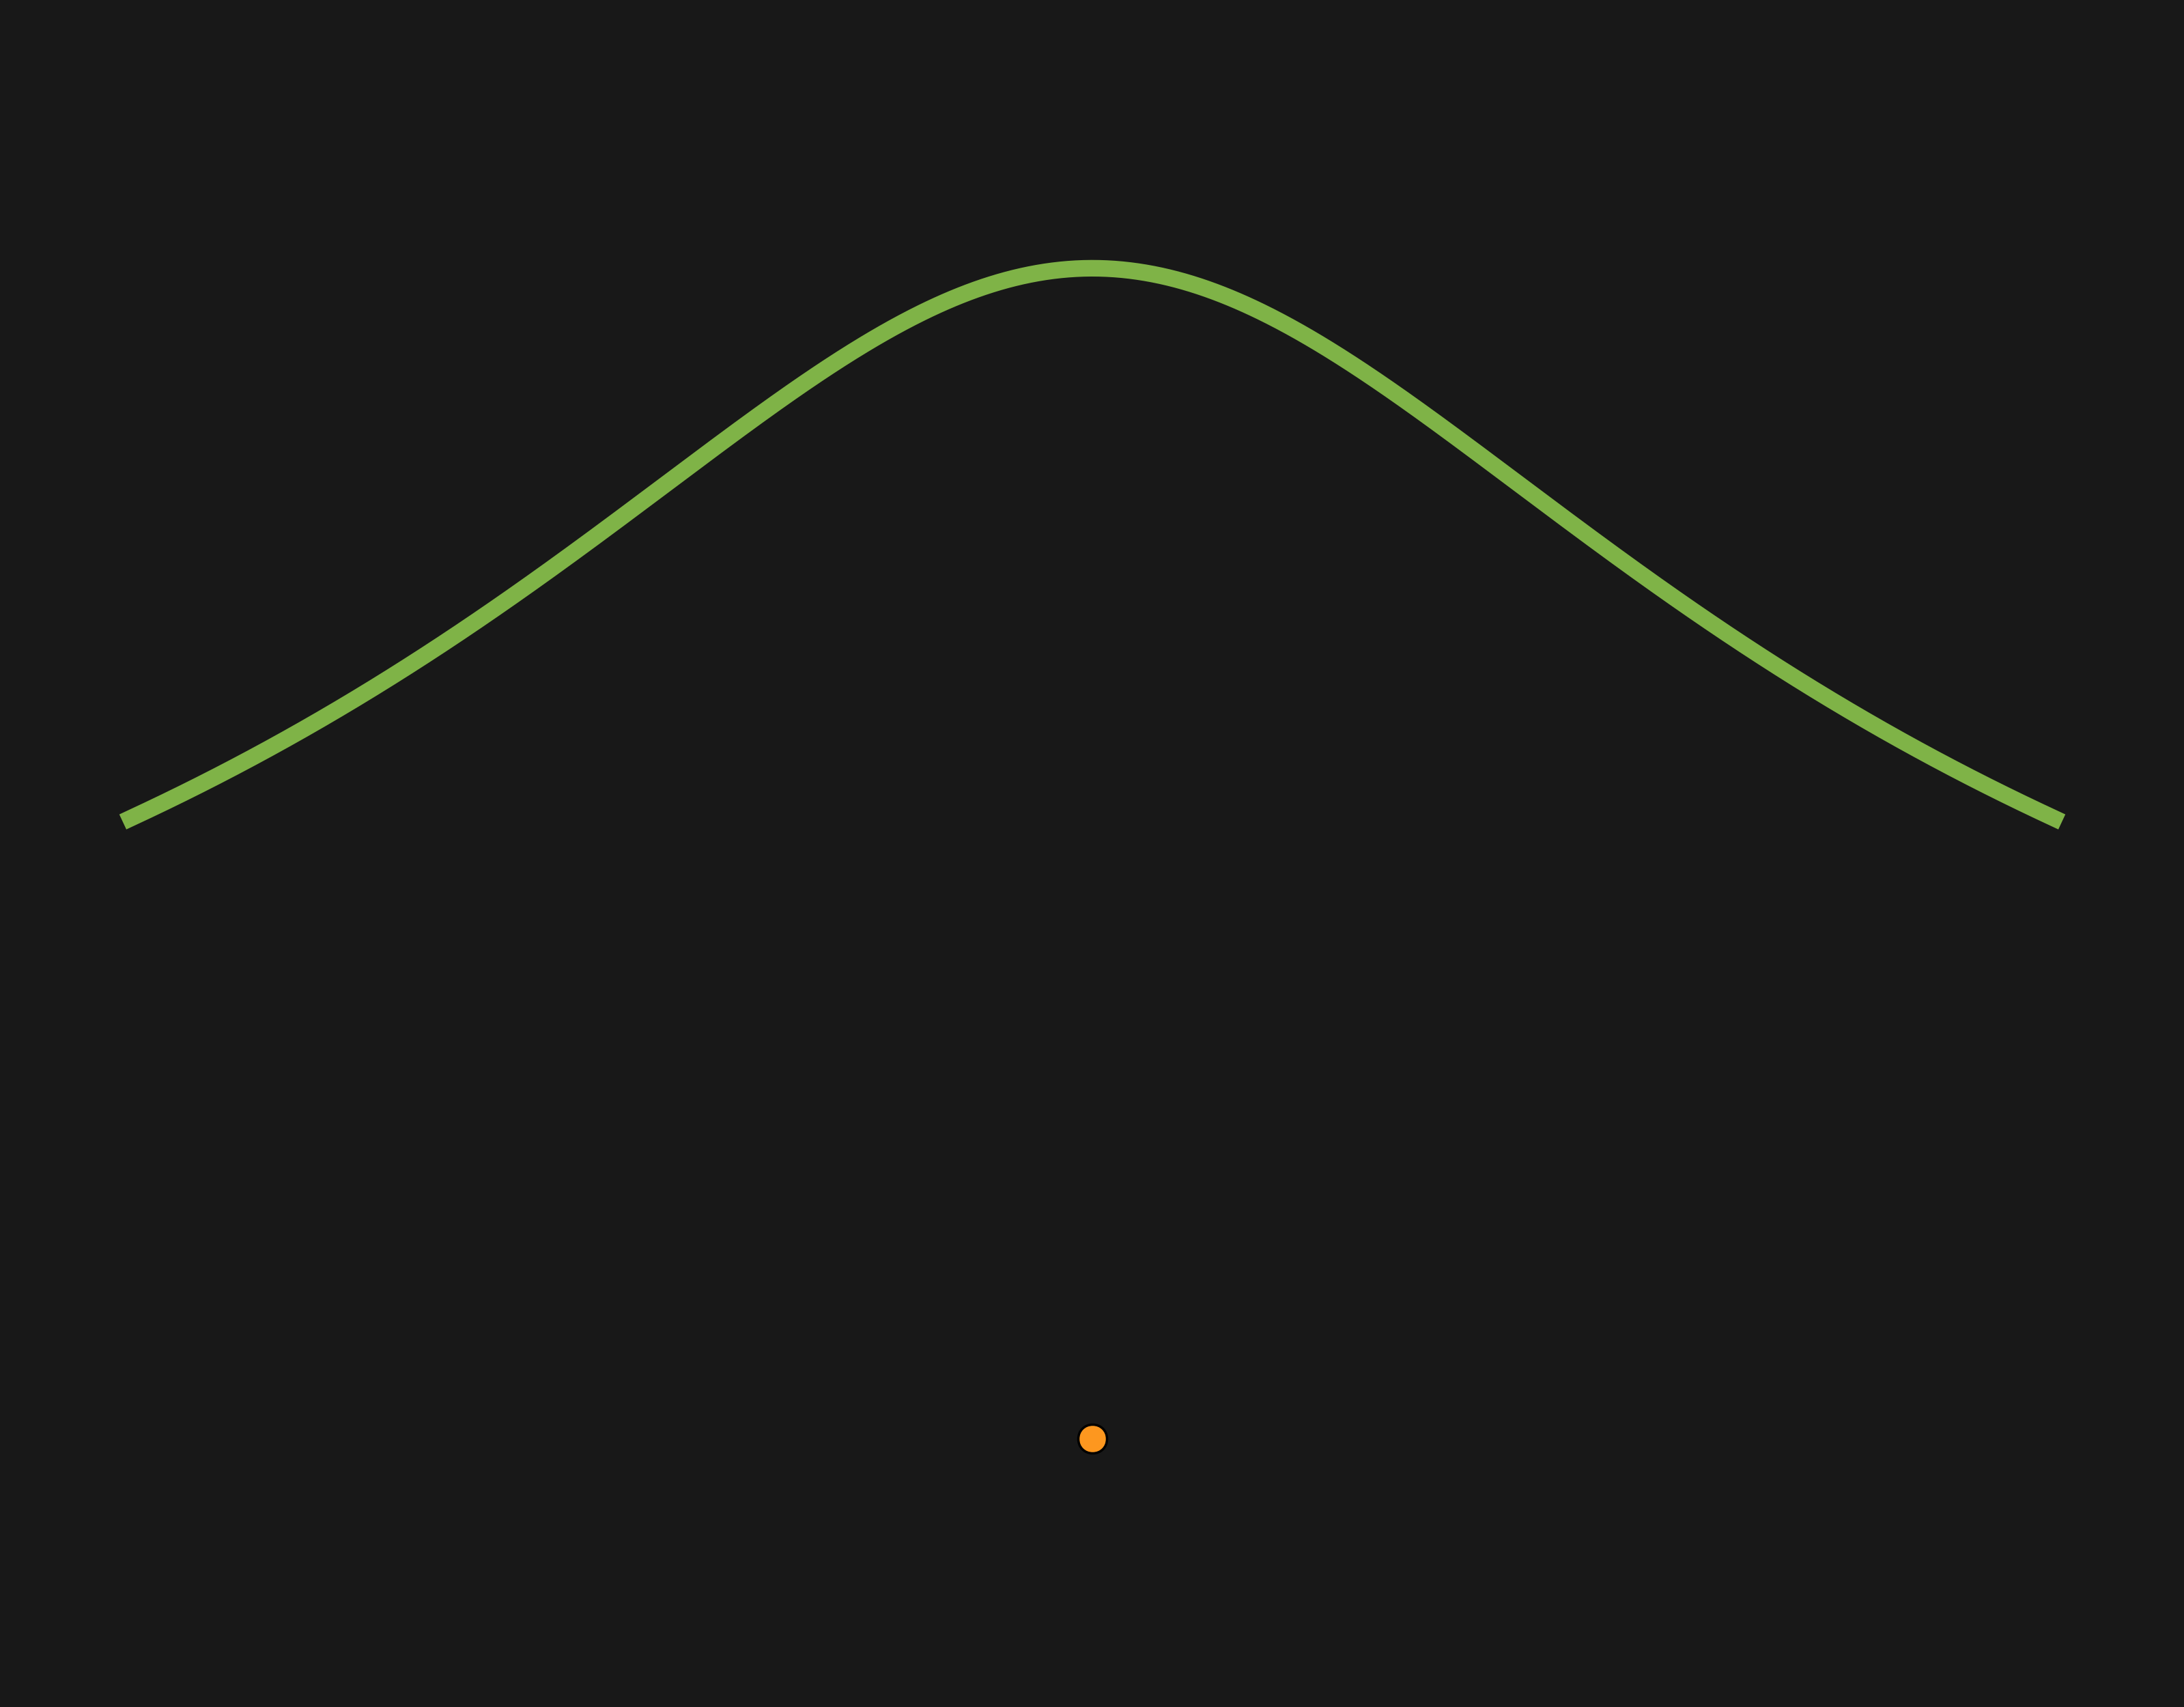
\includegraphics[width=0.2\textwidth]{inversemultiquadric.png}} \\
        \hline Inverse Quadratic & $\frac{1}{1+(\epsilon r)^2}$  & \parbox[c]{1em}{
      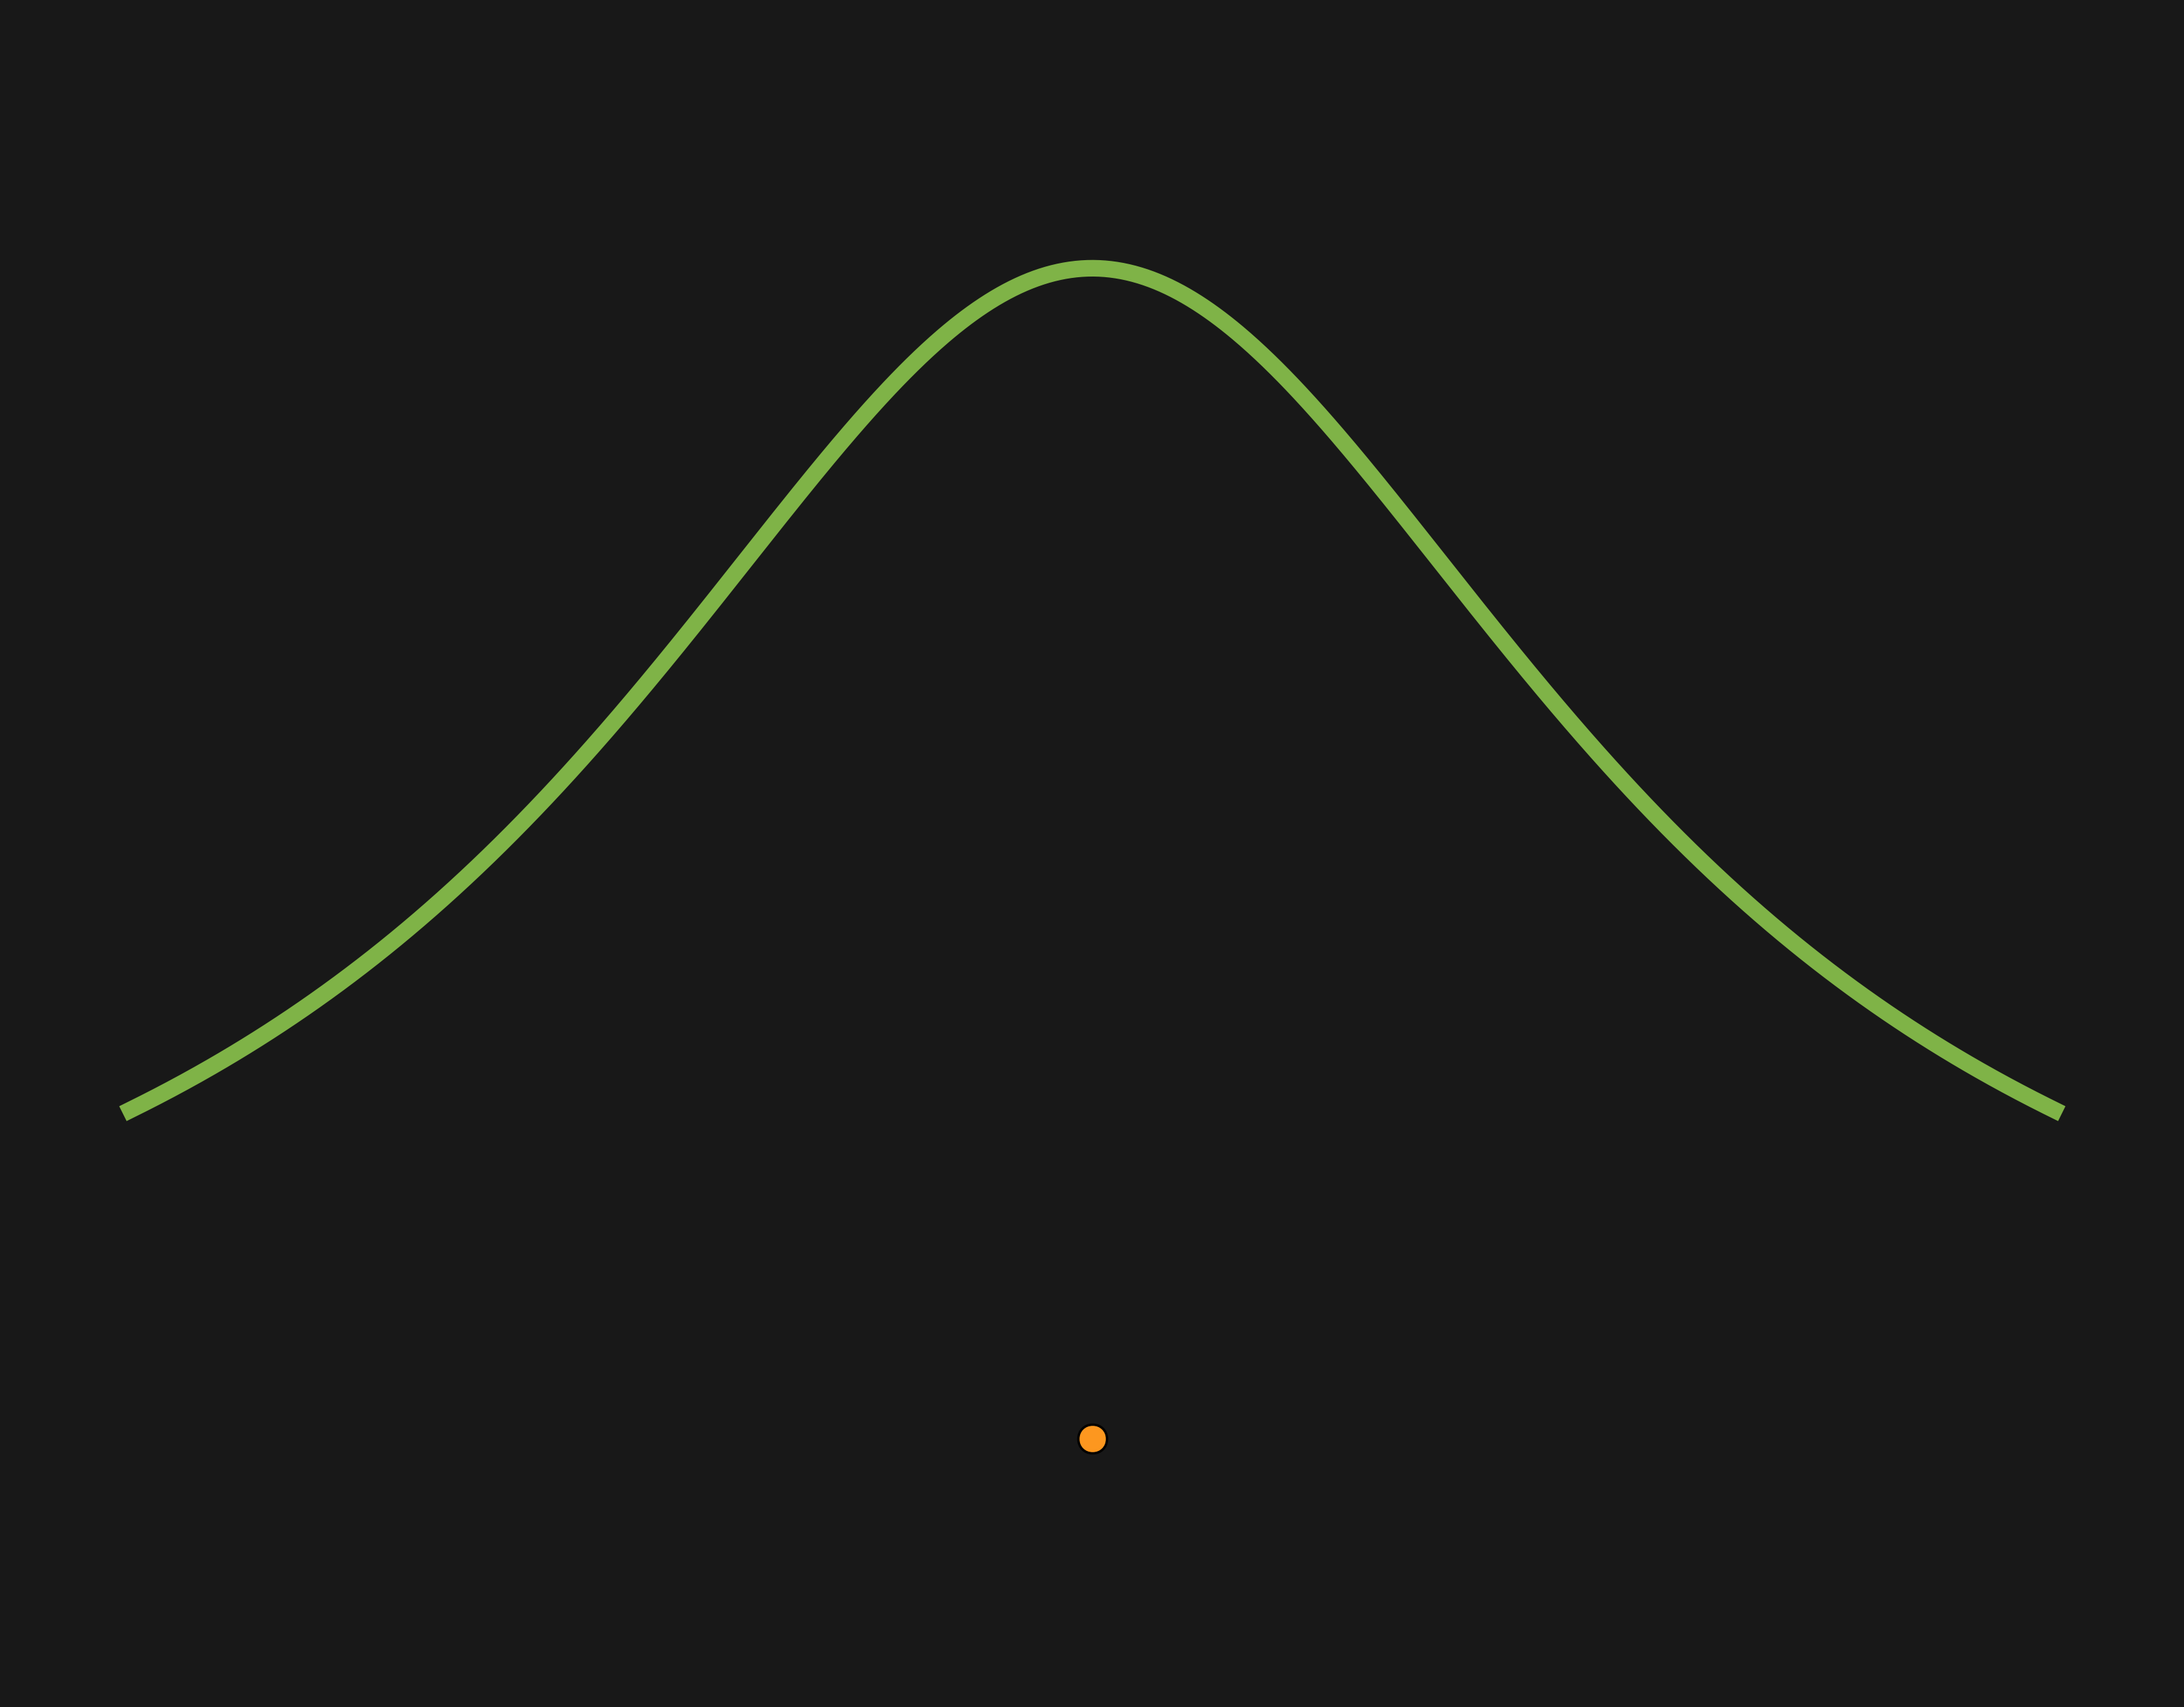
\includegraphics[width=0.2\textwidth]{inversequadratic.png}} \\
       \hline Gaussian & $e^{-(\epsilon r)^2}$  & \parbox[c]{1em}{
      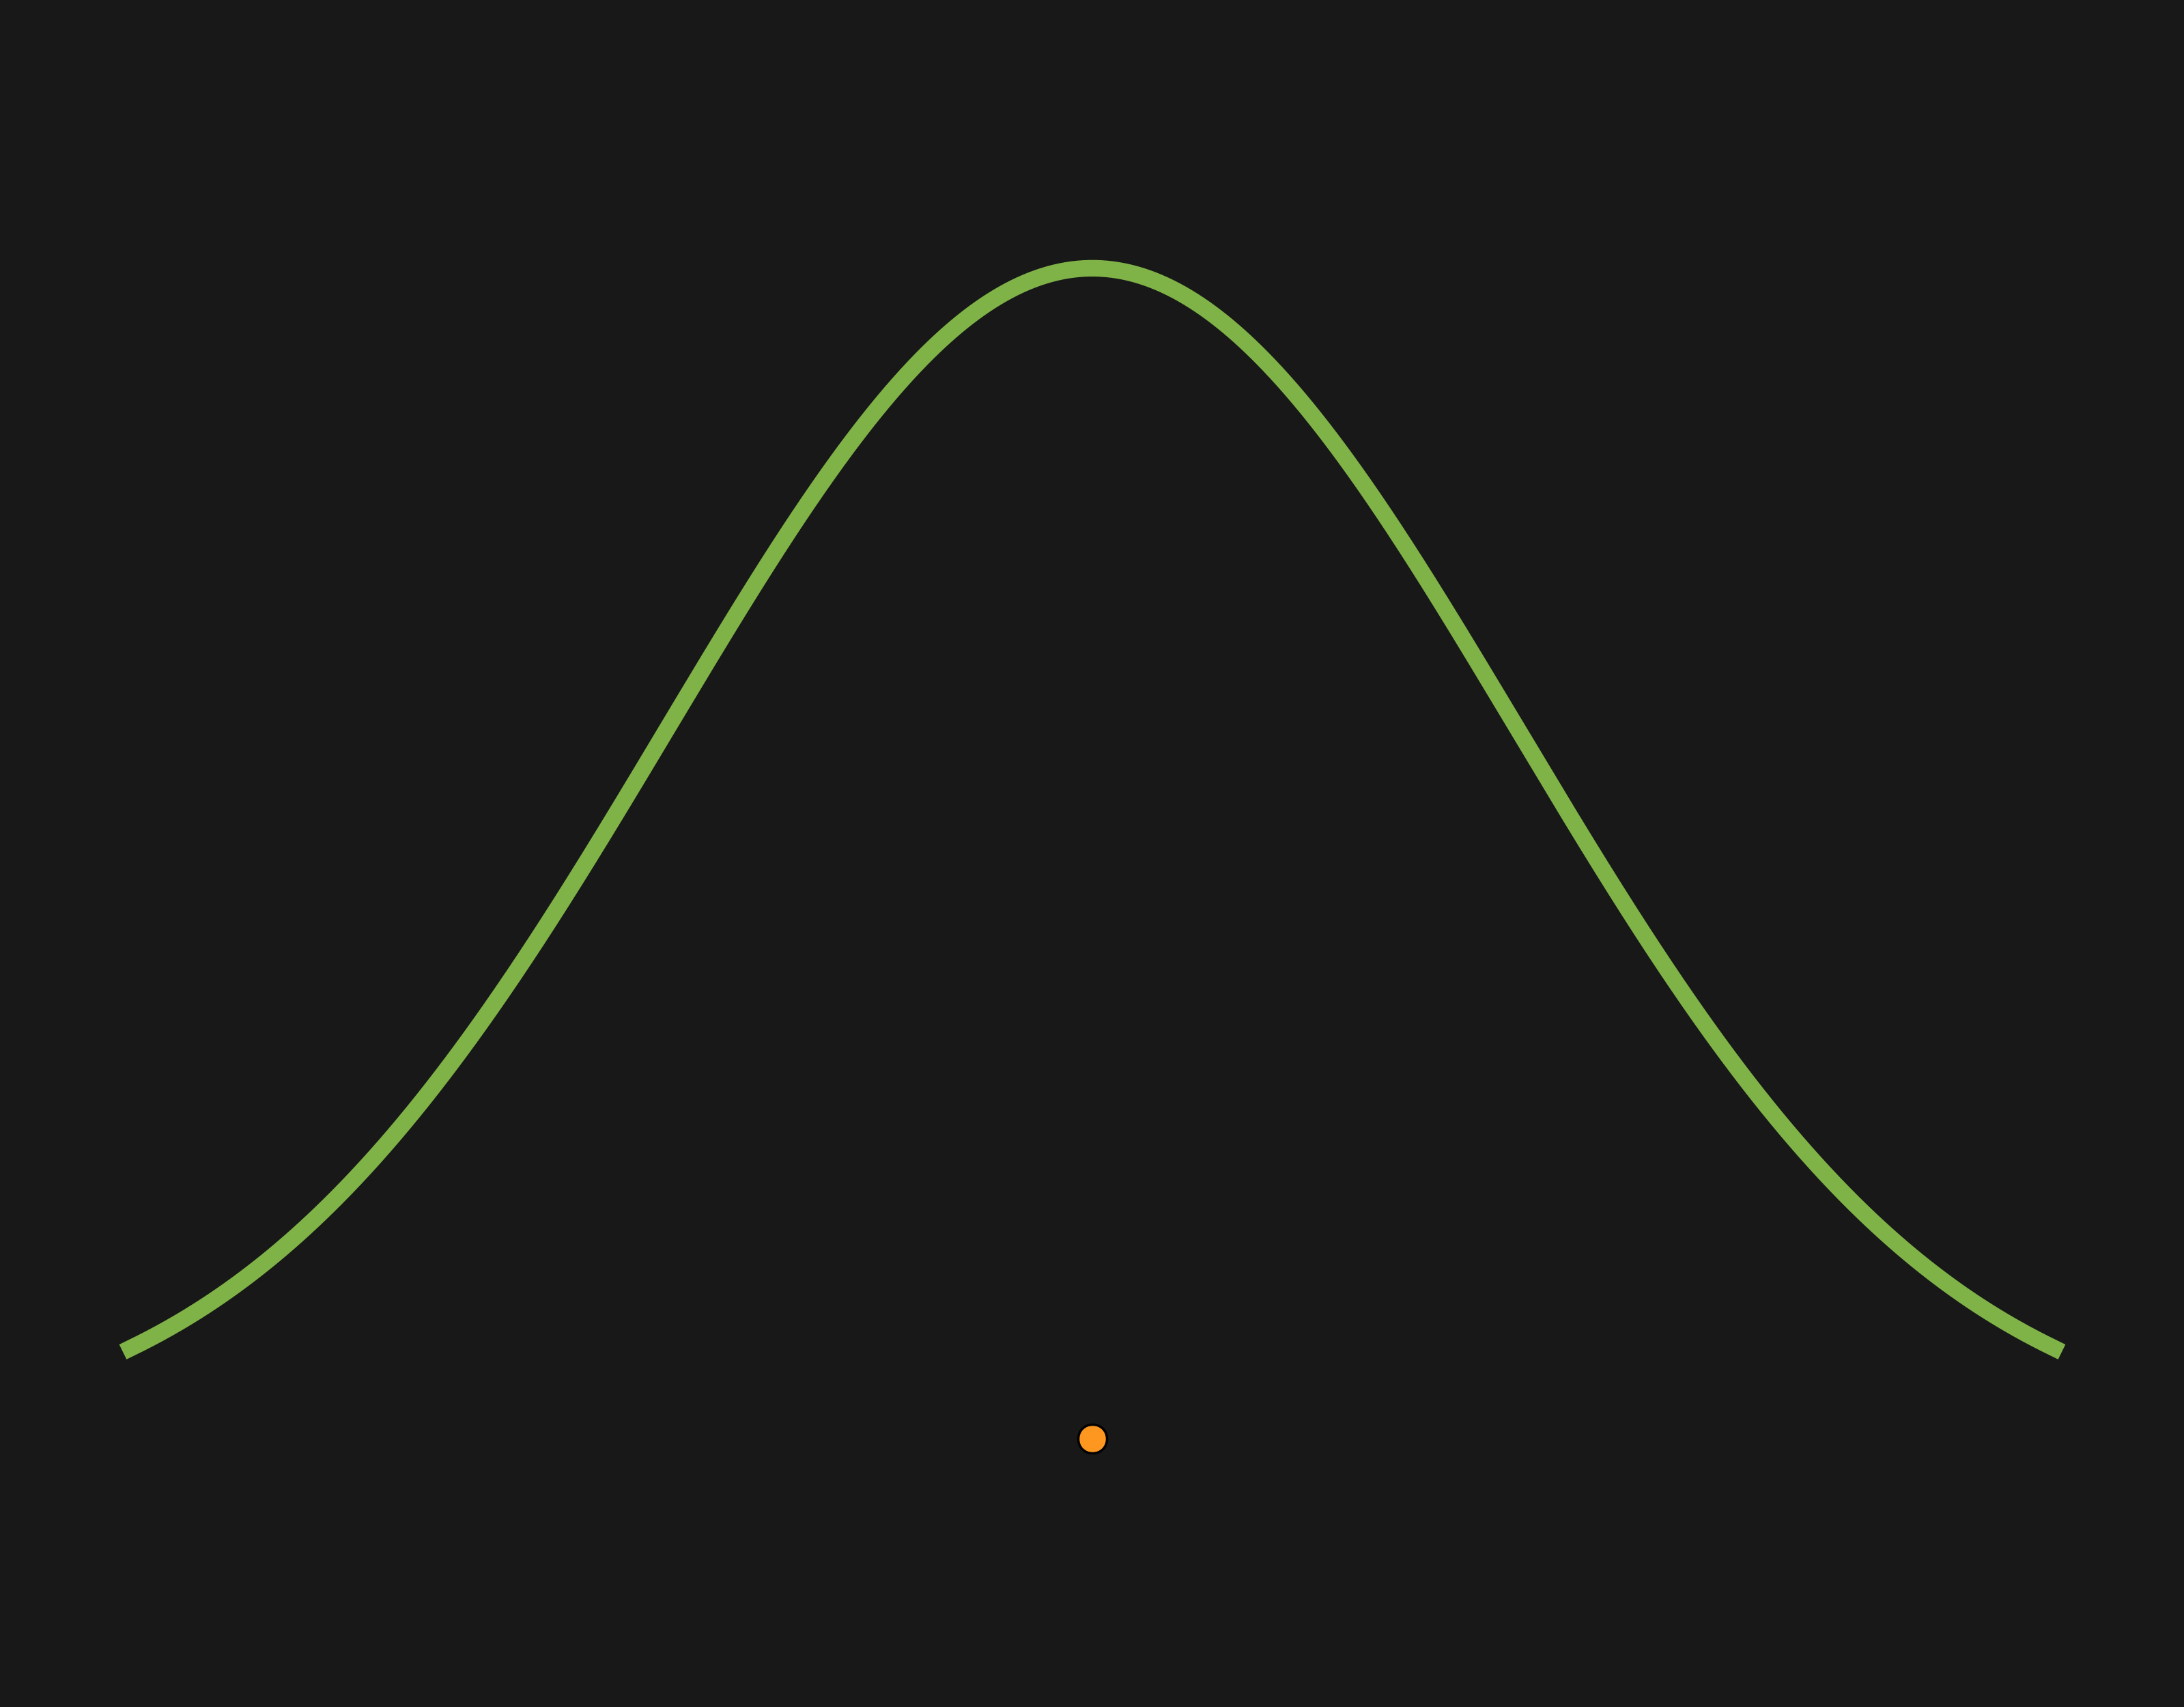
\includegraphics[width=0.2\textwidth]{gaussian.png}} \\
  \end{tabular}

\pause
\subt{Note:} One of these things is not like the others.

\note{Graphs of each kernel!}
\end{frame}

\begin{frame}{What About Well-Posed?}
Our interpolation matrix is no longer the distance matrix. Can we still expect well-posed?
\begin{equation*}
A=
\begin{bmatrix}
\phi_1(x_1) & \phi_1(x_2) & \cdots & \phi_1(x_N)\\
\phi_2(x_1) & \phi_2(x_2)& \cdots & \phi_2(x_N)\\
\vdots & \vdots & \ddots & \vdots\\
\phi_N(x_1) & \phi_N(x_2)& \cdots & \phi_N(x_N)
\end{bmatrix}
\end{equation*}
\pause

\subt{A New, Less Sexy Condition:}

If interpolation matrix, A, is symmetric \subt{positive-definite}, then A is nonsingular and our system is well-posed.

\note{}
\end{frame}

\begin{frame}{Positive-Definite}
Our matrix, A, is \subt{positive-definite} if
\begin{align*}
& t^TAt>0 & \forall t=\left[ t_1, t_2, \mathellipsis, t_n\right]\neq 0 \in \mathbb{R}^n
\end{align*}

Which results from a \subt{positive-definite} kernel, $\phi: \mathbb{R}^s \times \mathbb{R}^s \rightarrow \mathbb{R}$:
\begin{align*}
&\sum_{i=1}^N \sum_{j=1}^N \phi(||x-x_i||)t_i\bar{t_j}>0 &\forall t=\left[ t_1, t_2, \mathellipsis, t_n\right]\neq 0 \in \mathbb{C}^n
\end{align*}

\subt{Useful Properties of Positive Definite Matricies}
\bi
\item All positive eigenvalues $\implies$ Non-Singular
\item More efficient solving methods, e.g., Cholskey factorization
\ei

\note{}
\end{frame}

\begin{frame}{Radial Basis Kernels}


% \begin{table}
%   [ht] 
  \begin{tabular}
      {lll}  Common RBF Kernels  & $\phi(r)$\\
      \hline \cellcolor{orange} Multiquadric & $\sqrt{1+(\epsilon r)^2}$  & \parbox[c]{1em}{
      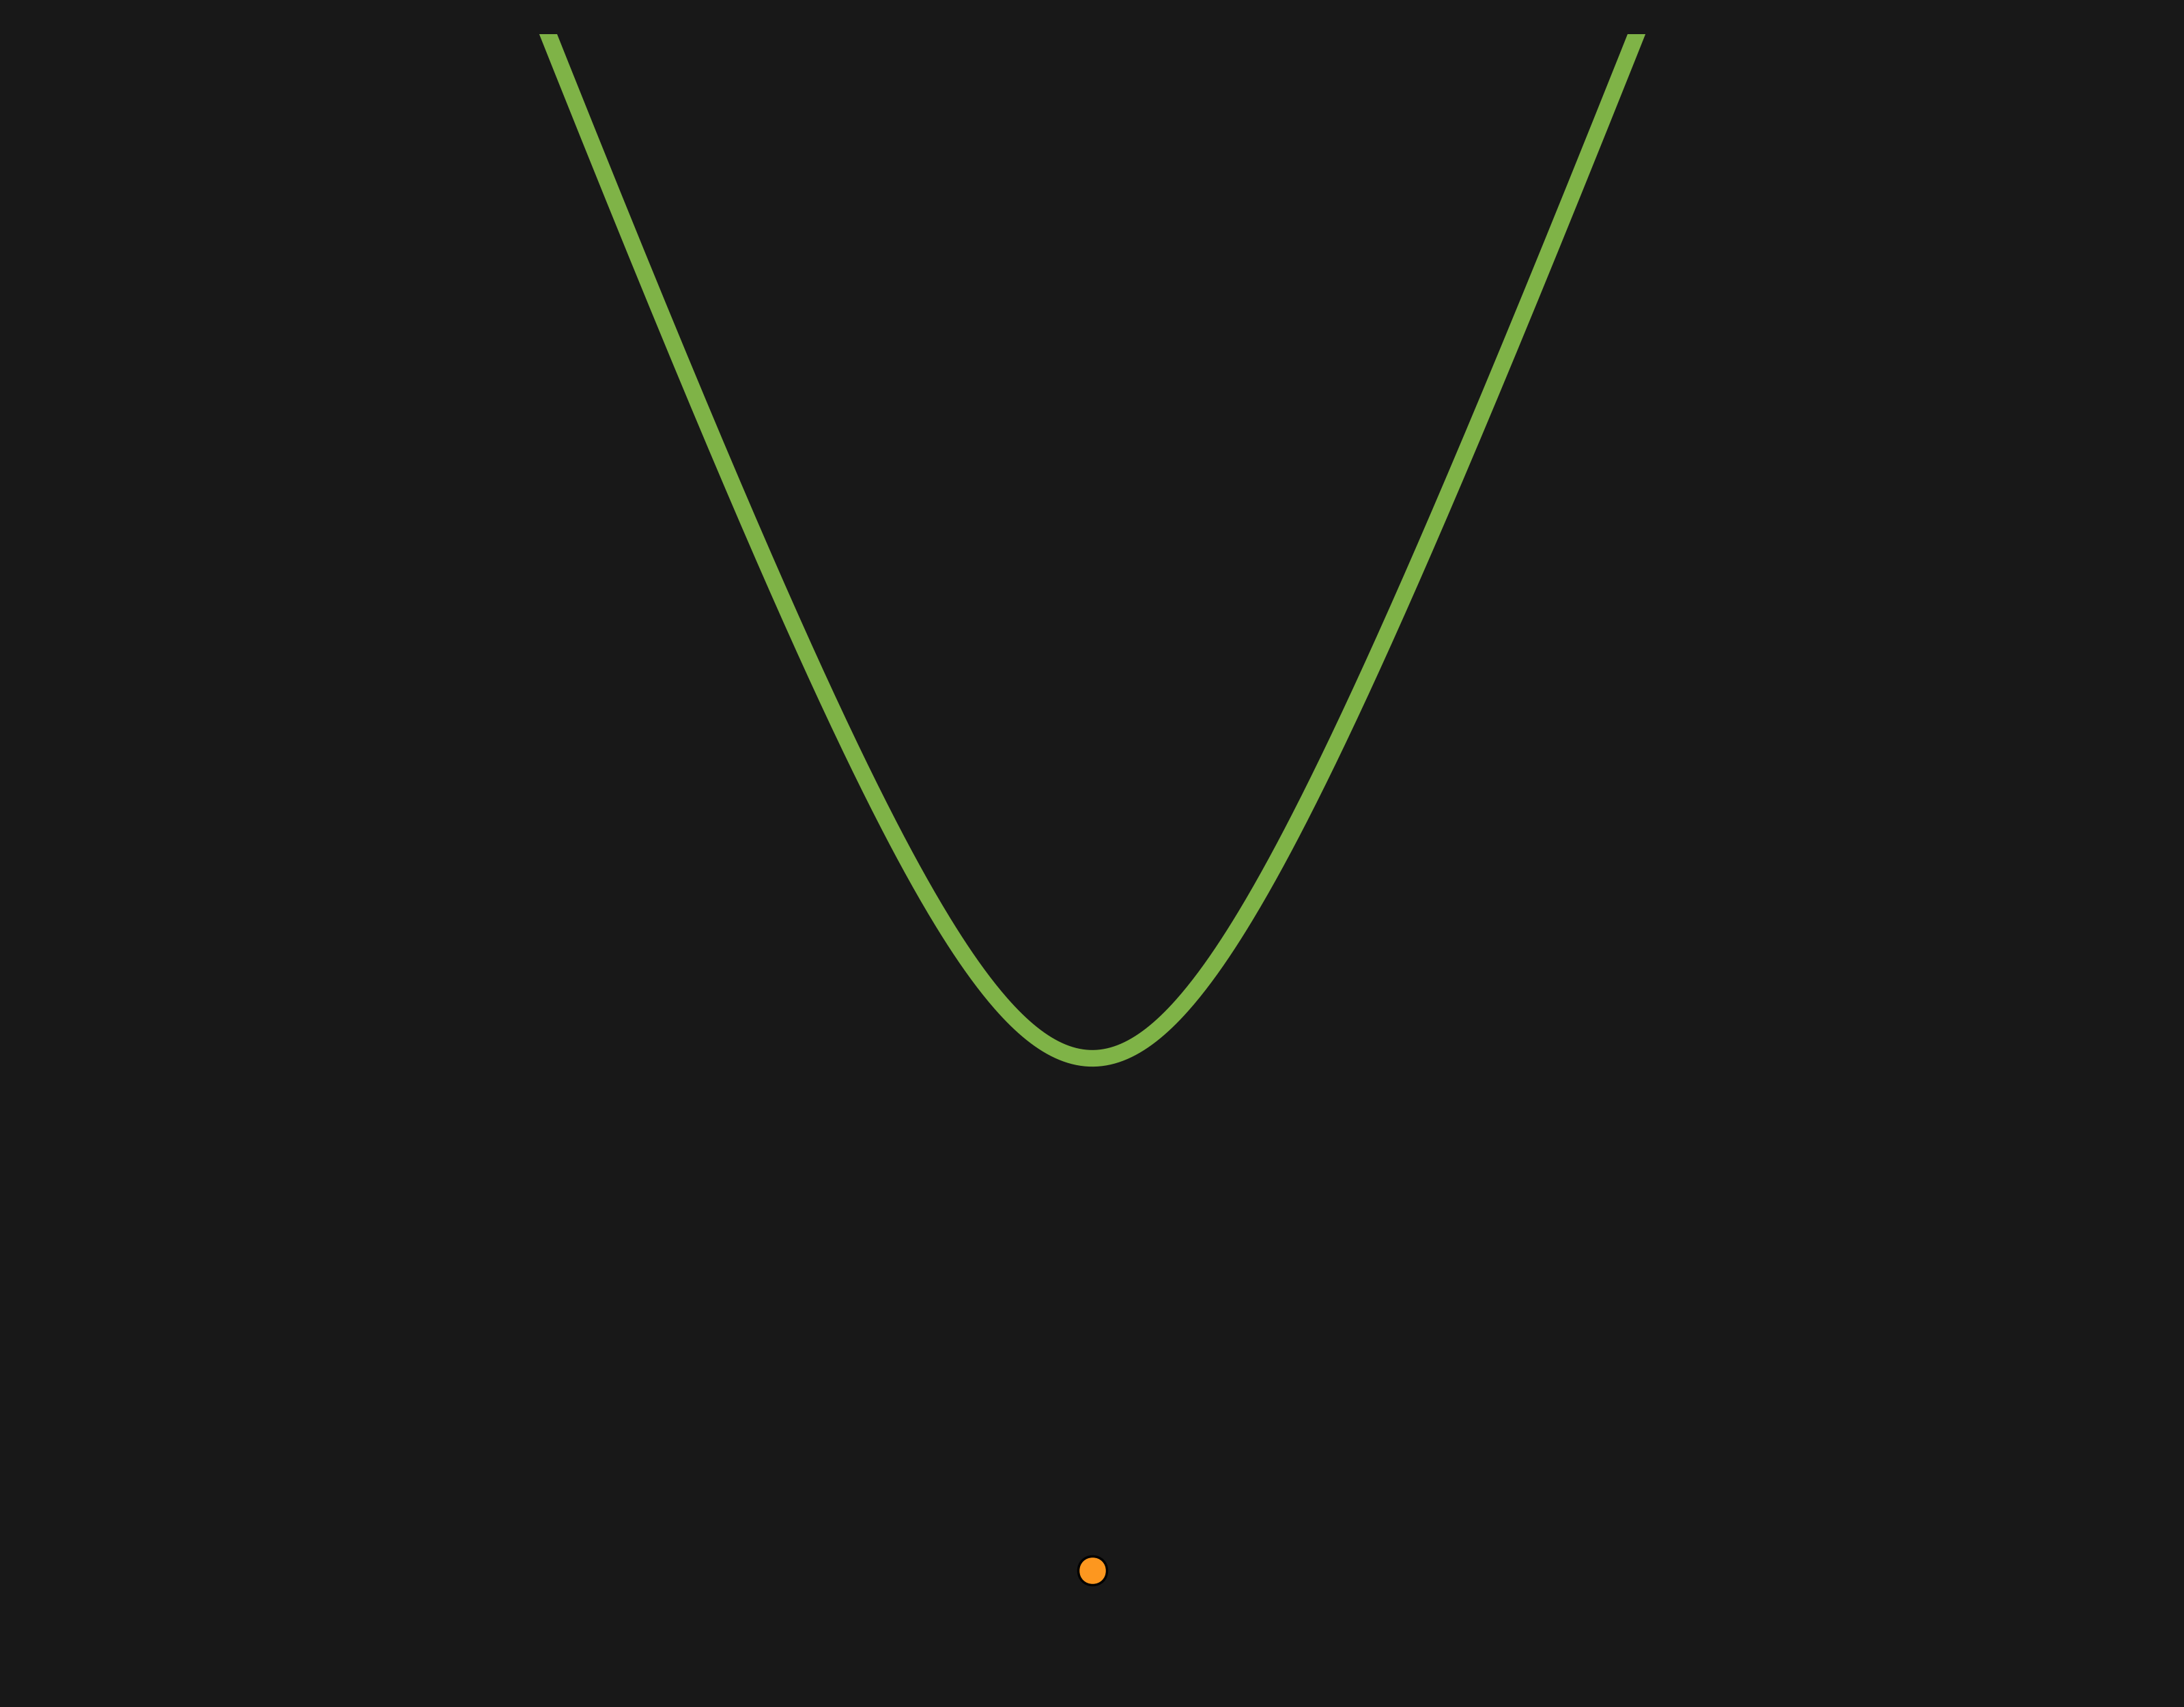
\includegraphics[width=0.1\textwidth]{multiquadric.png}} \\
      \hline \cellcolor{green} Inverse Multiquadric & $\frac{1}{\sqrt{1+(\epsilon r)^2}}$  & \parbox[c]{1em}{
      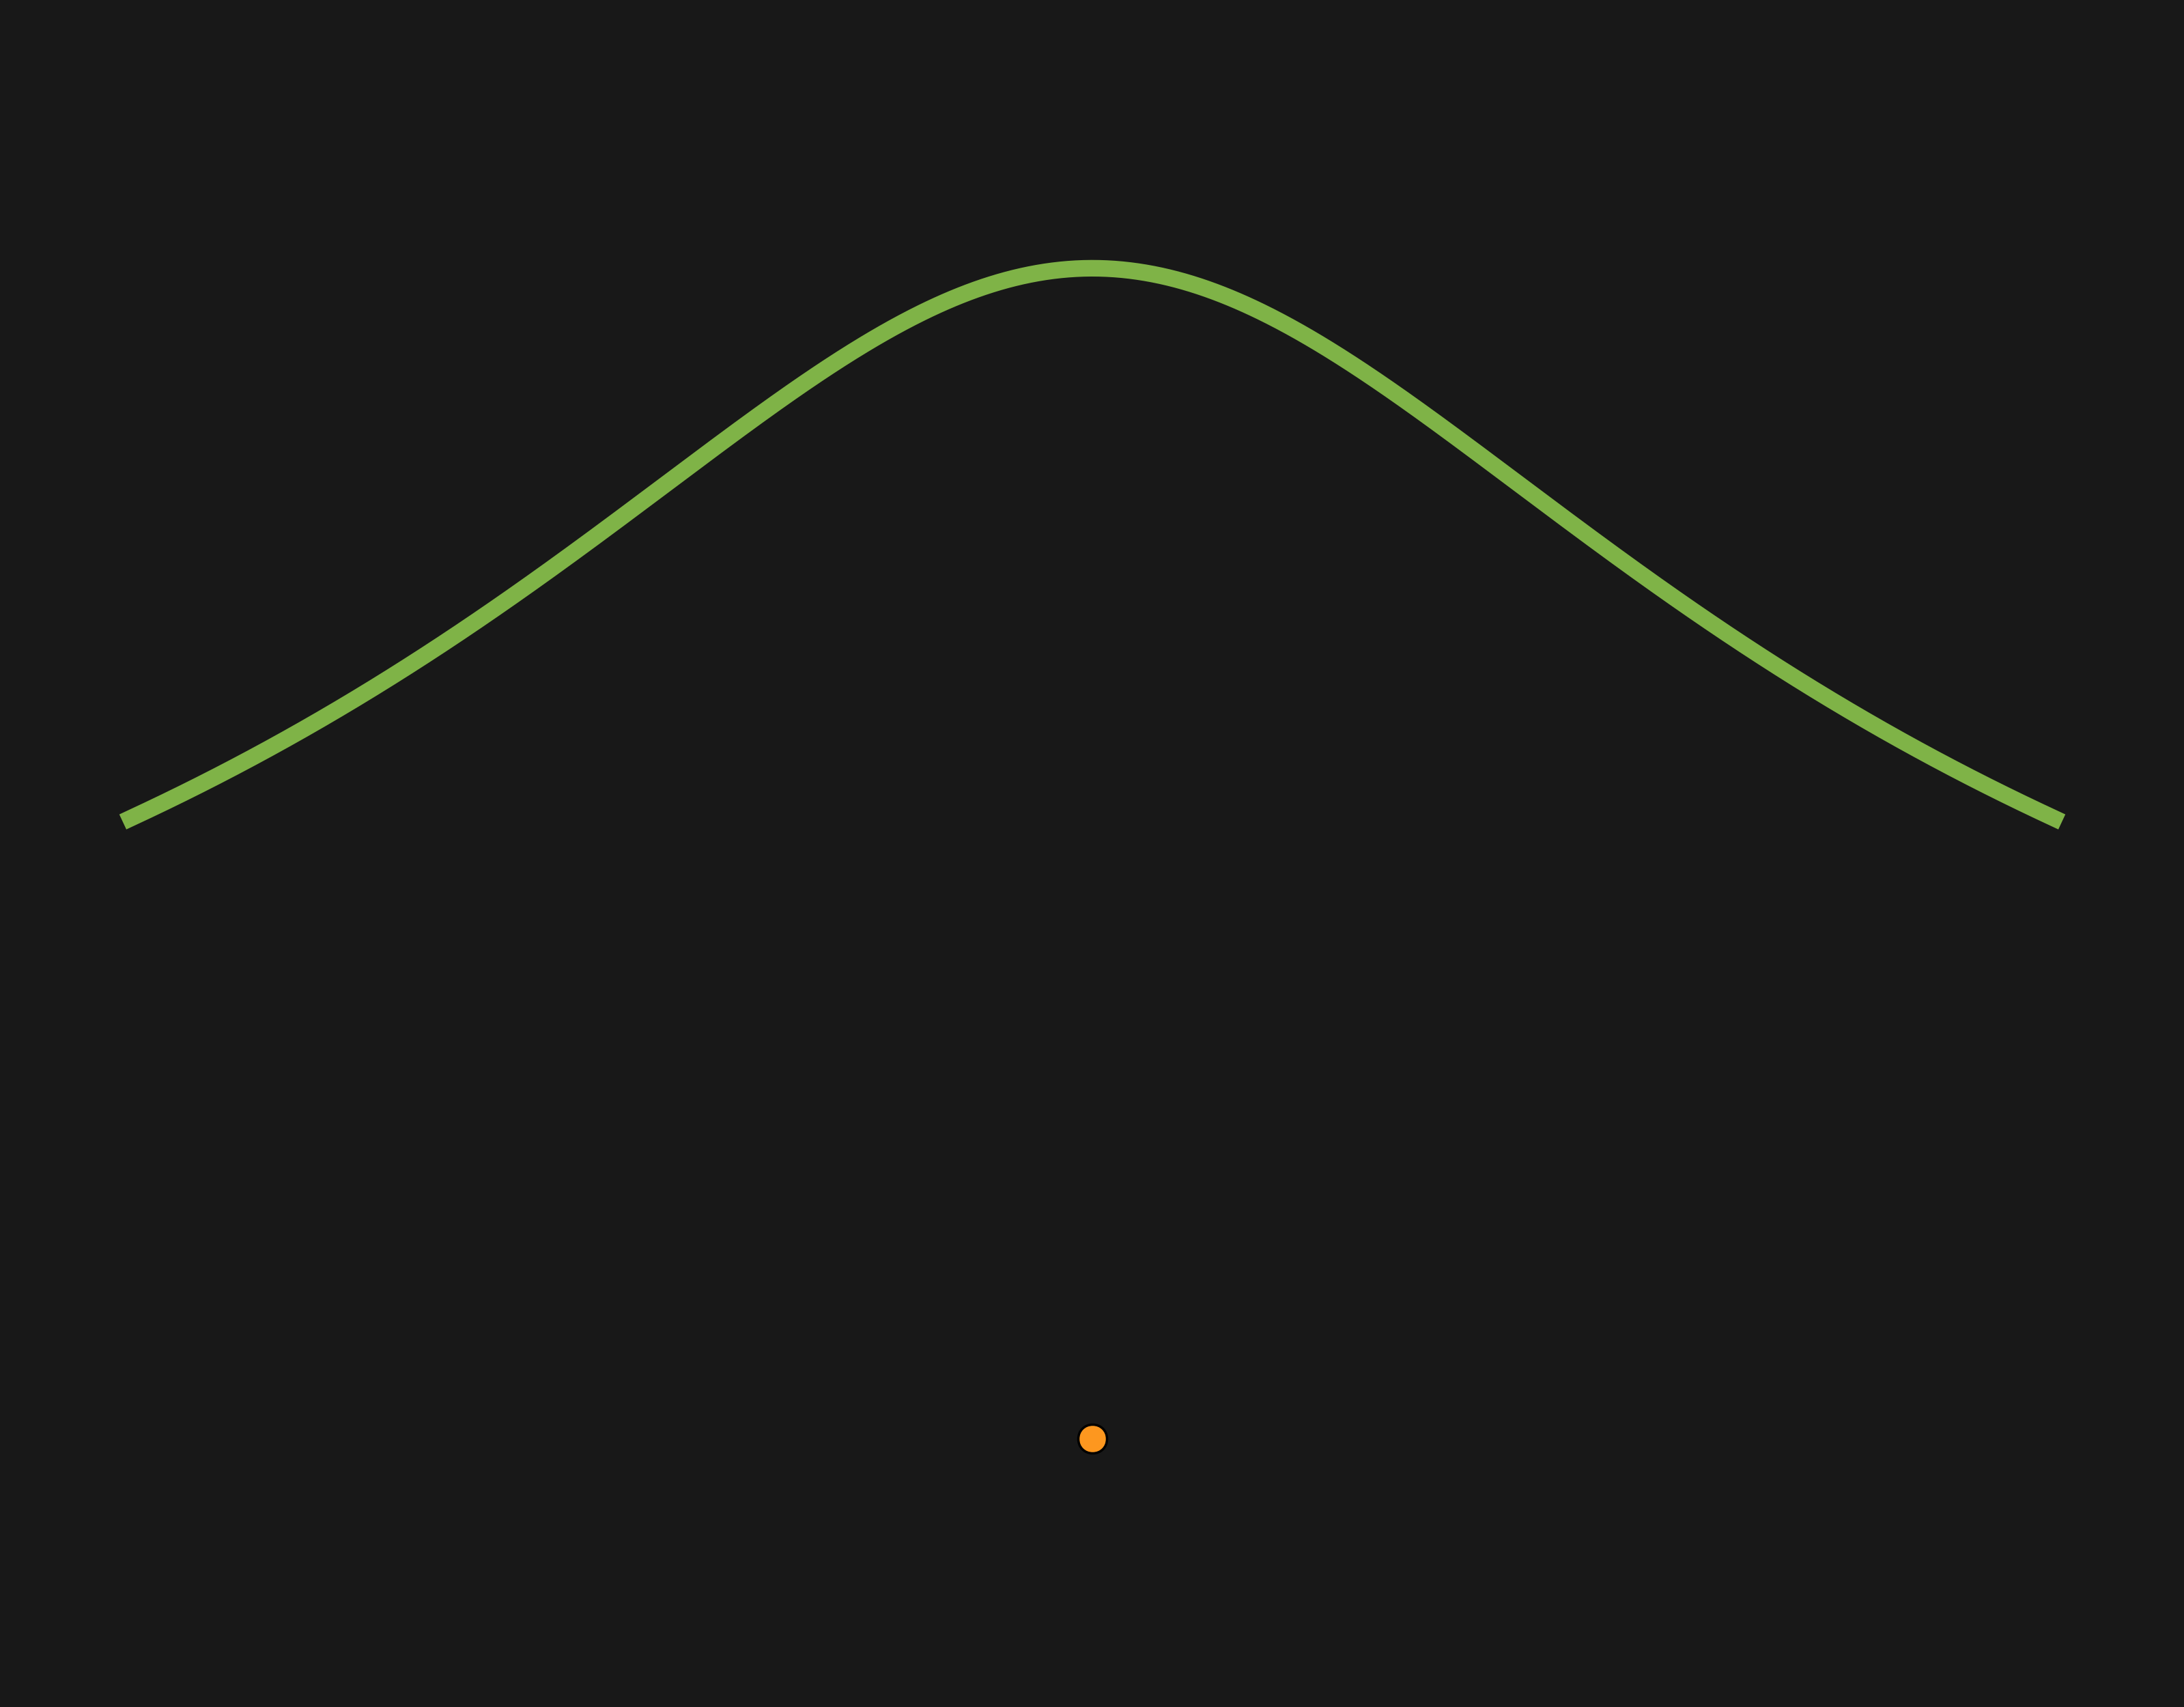
\includegraphics[width=0.1\textwidth]{inversemultiquadric.png}} \\
        \hline \cellcolor{green} Inverse Quadratic & $\frac{1}{1+(\epsilon r)^2}$  & \parbox[c]{1em}{
      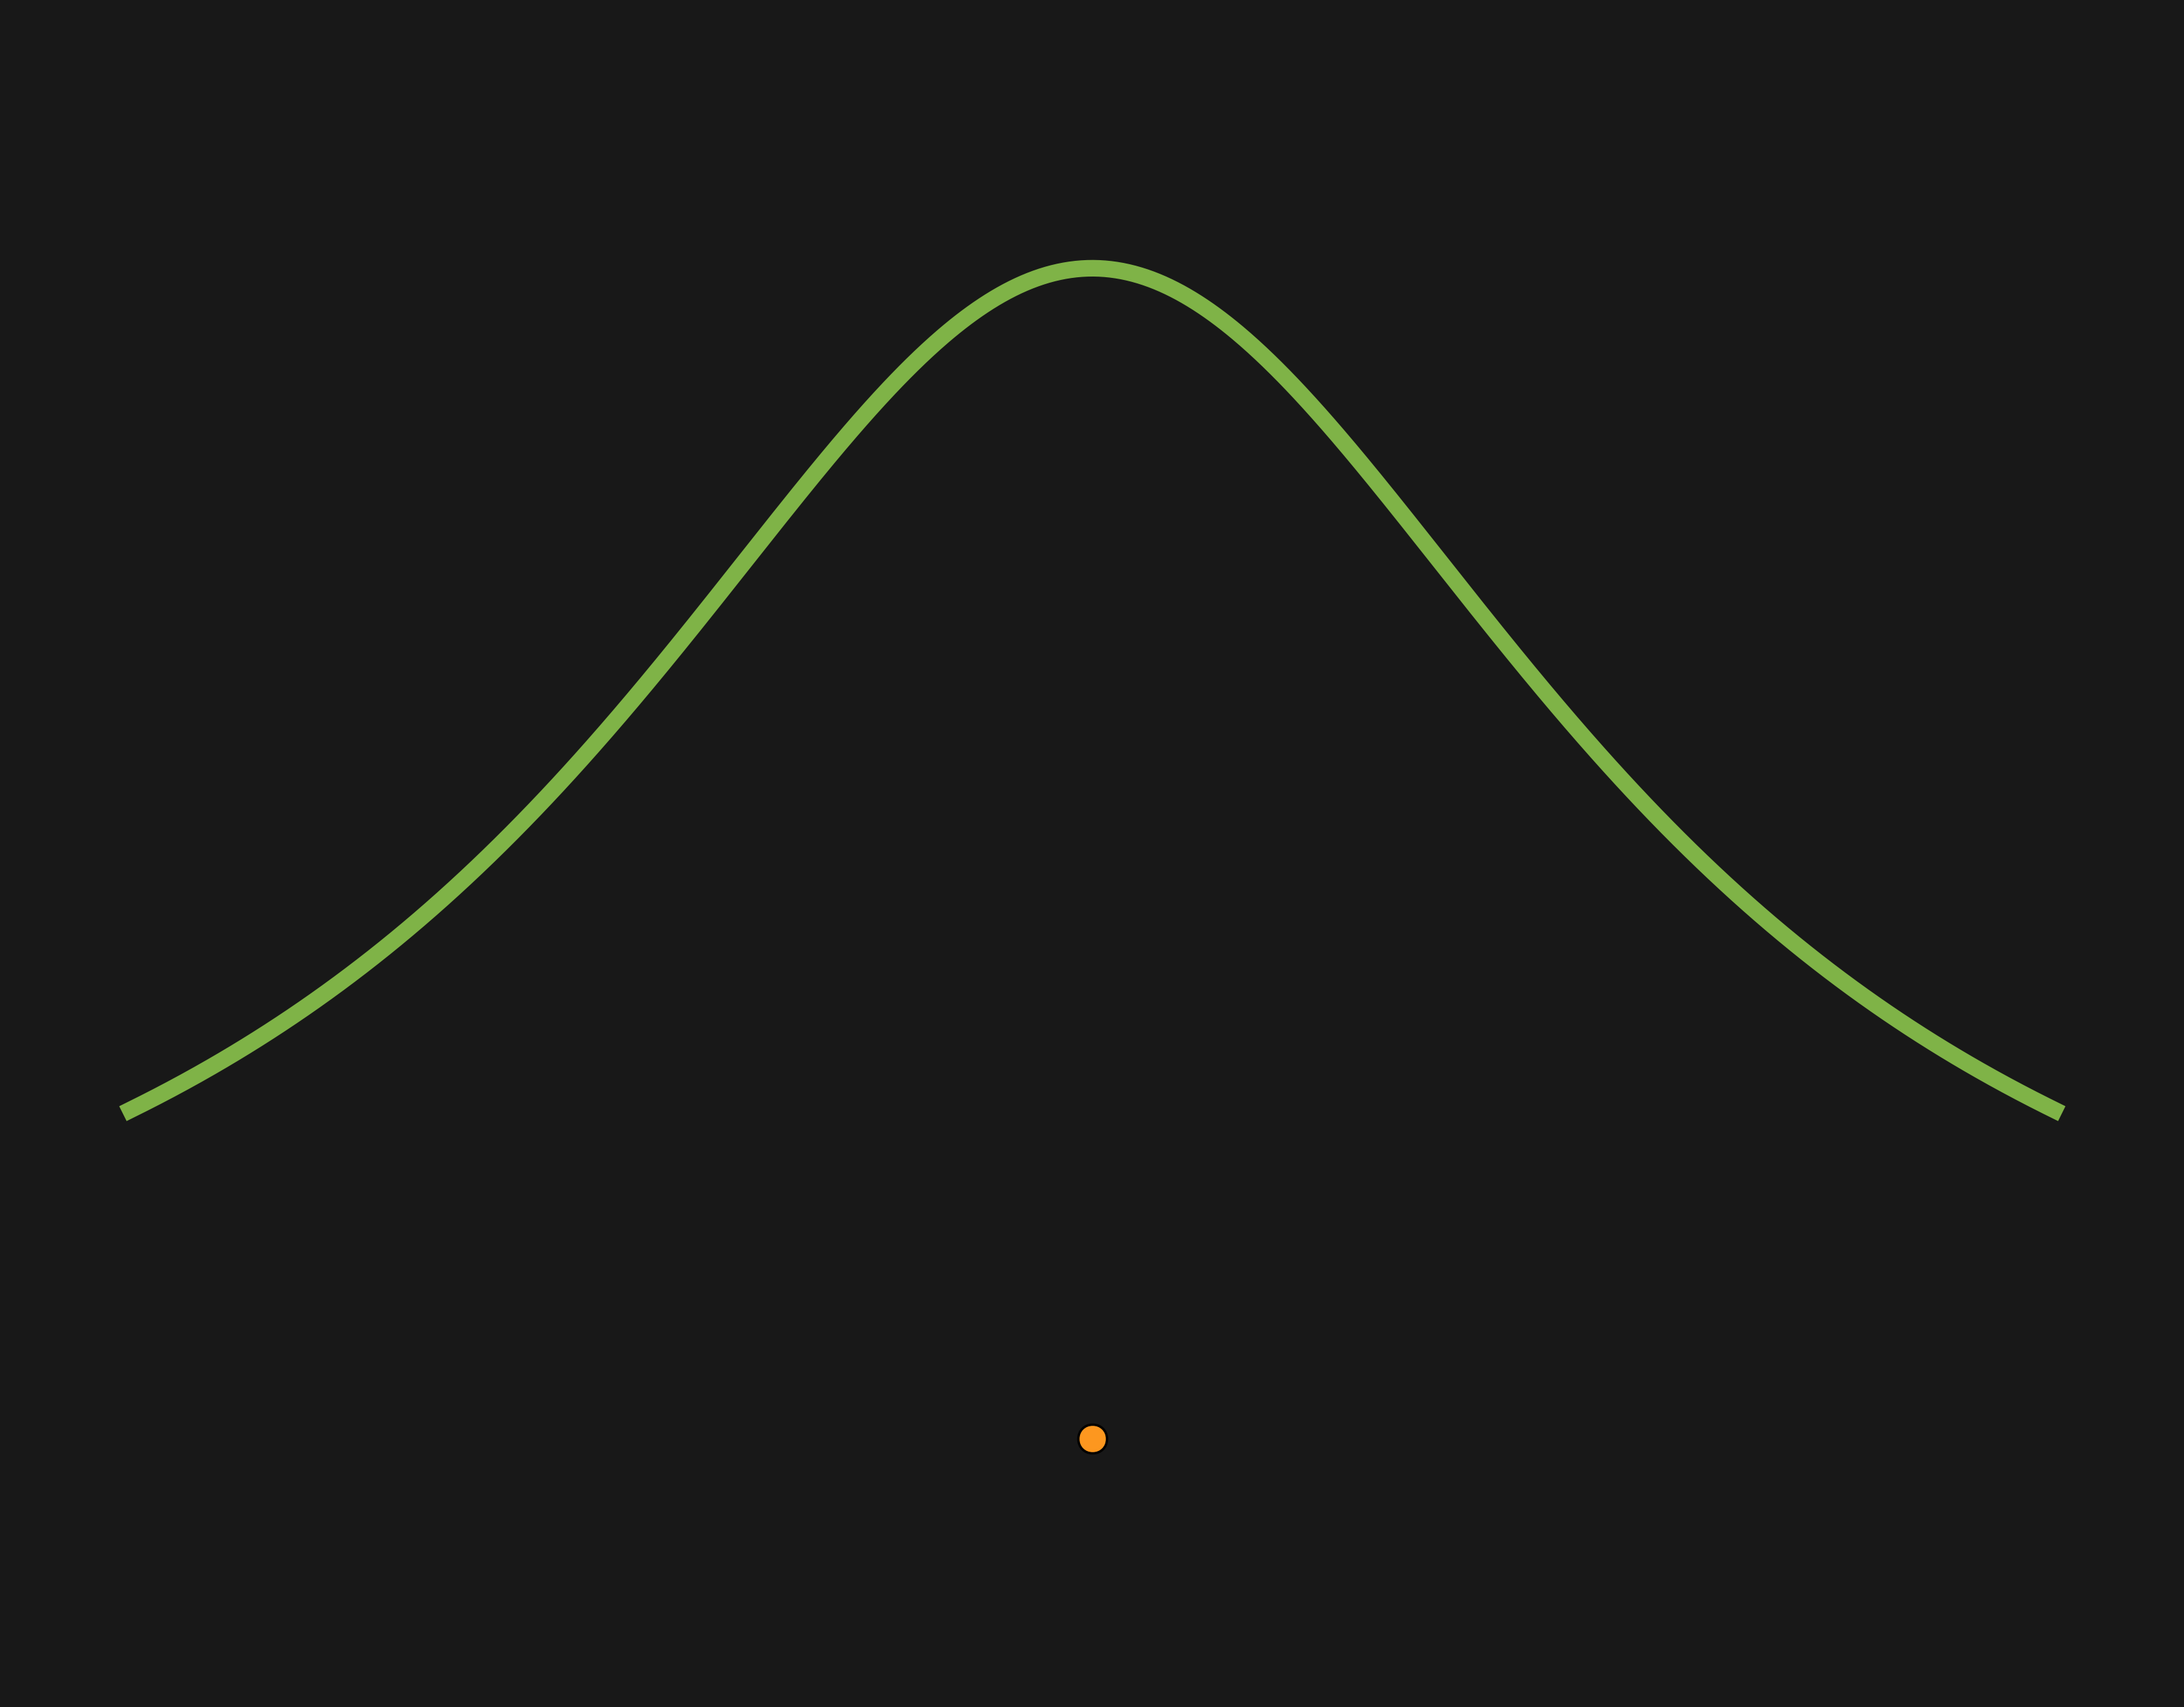
\includegraphics[width=0.1\textwidth]{inversequadratic.png}} \\
       \hline \cellcolor{green} Gaussian & $e^{-(\epsilon r)^2}$  & \parbox[c]{1em}{
      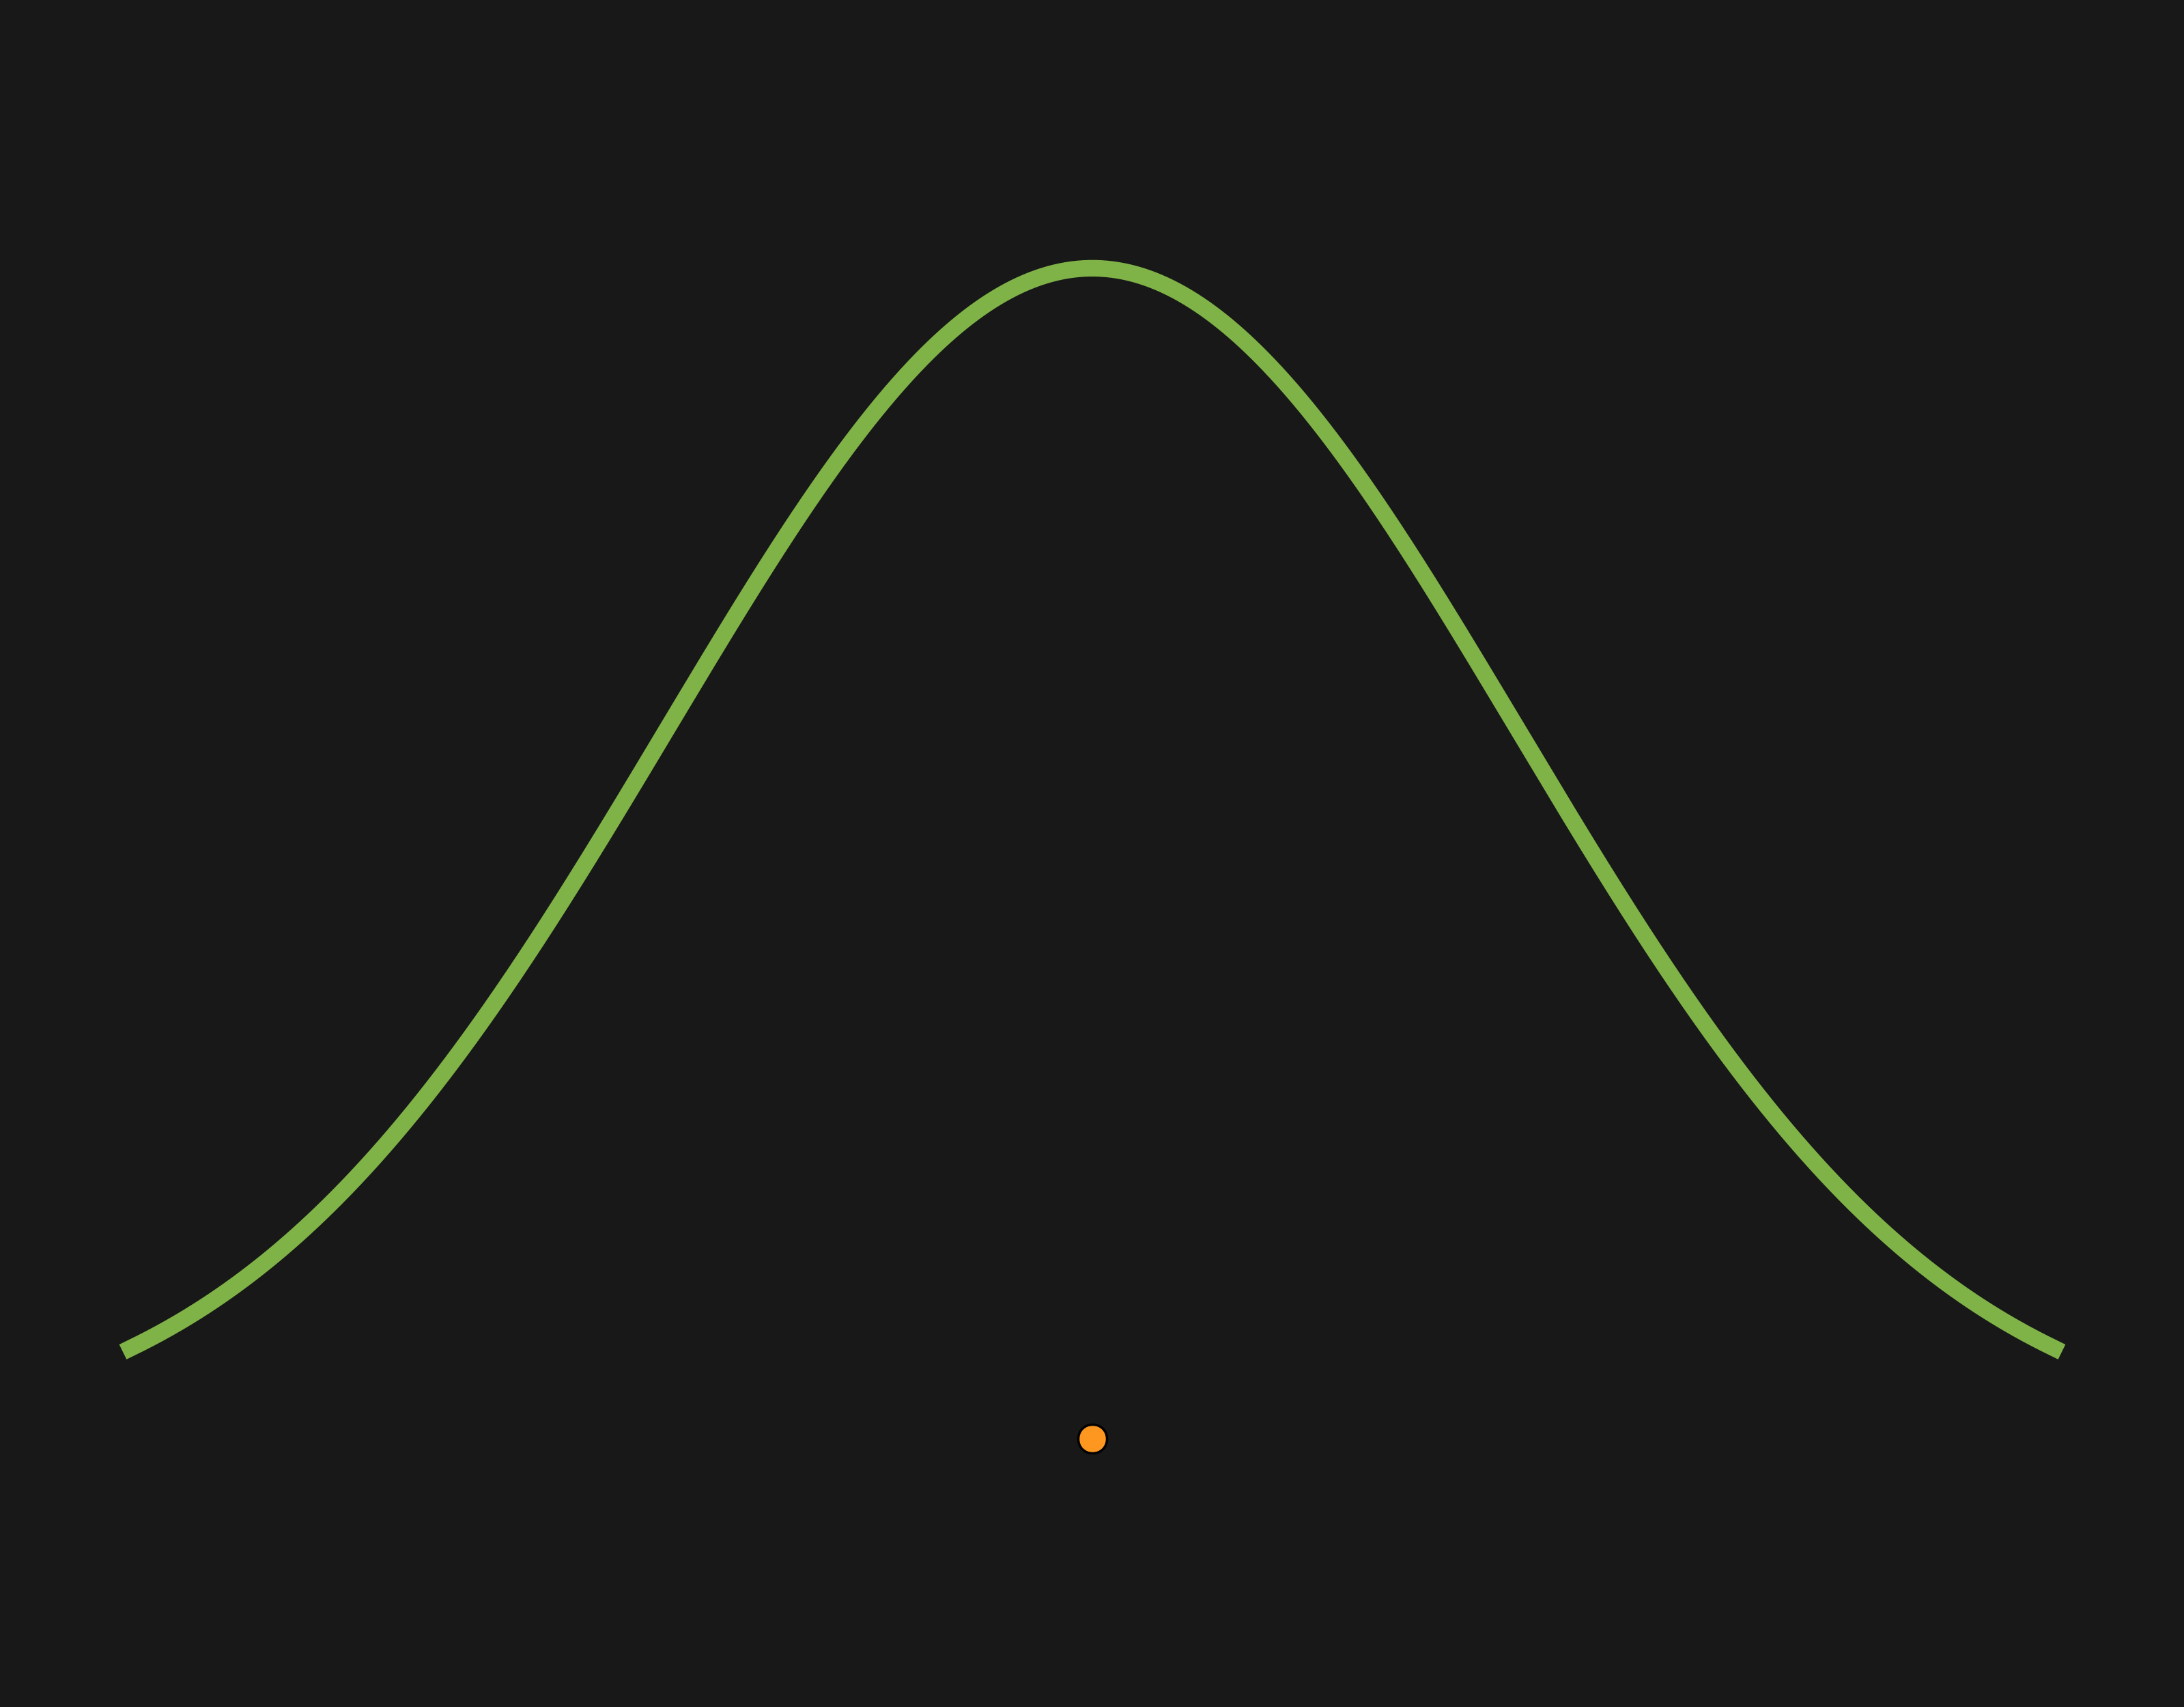
\includegraphics[width=0.1\textwidth]{gaussian.png}} \\
  \end{tabular}
\bigskip

Hardy's Multiquadric Kernel is not \textcolor{green}{positive-definite}. However, it is conditionally \textcolor{orange}{negative-definite}.

\subt{Properties of Multiquadric Matrix}

\bi
\item One positive eigenvalue and $(n-1)$ negative eigenvalues $\implies$ Non-Singular
\item Not generally subject to positive-definite solving methods
\ei

\note{}
\end{frame}

\begin{frame}{Visualizing the RBF Method}

\begin{figure}
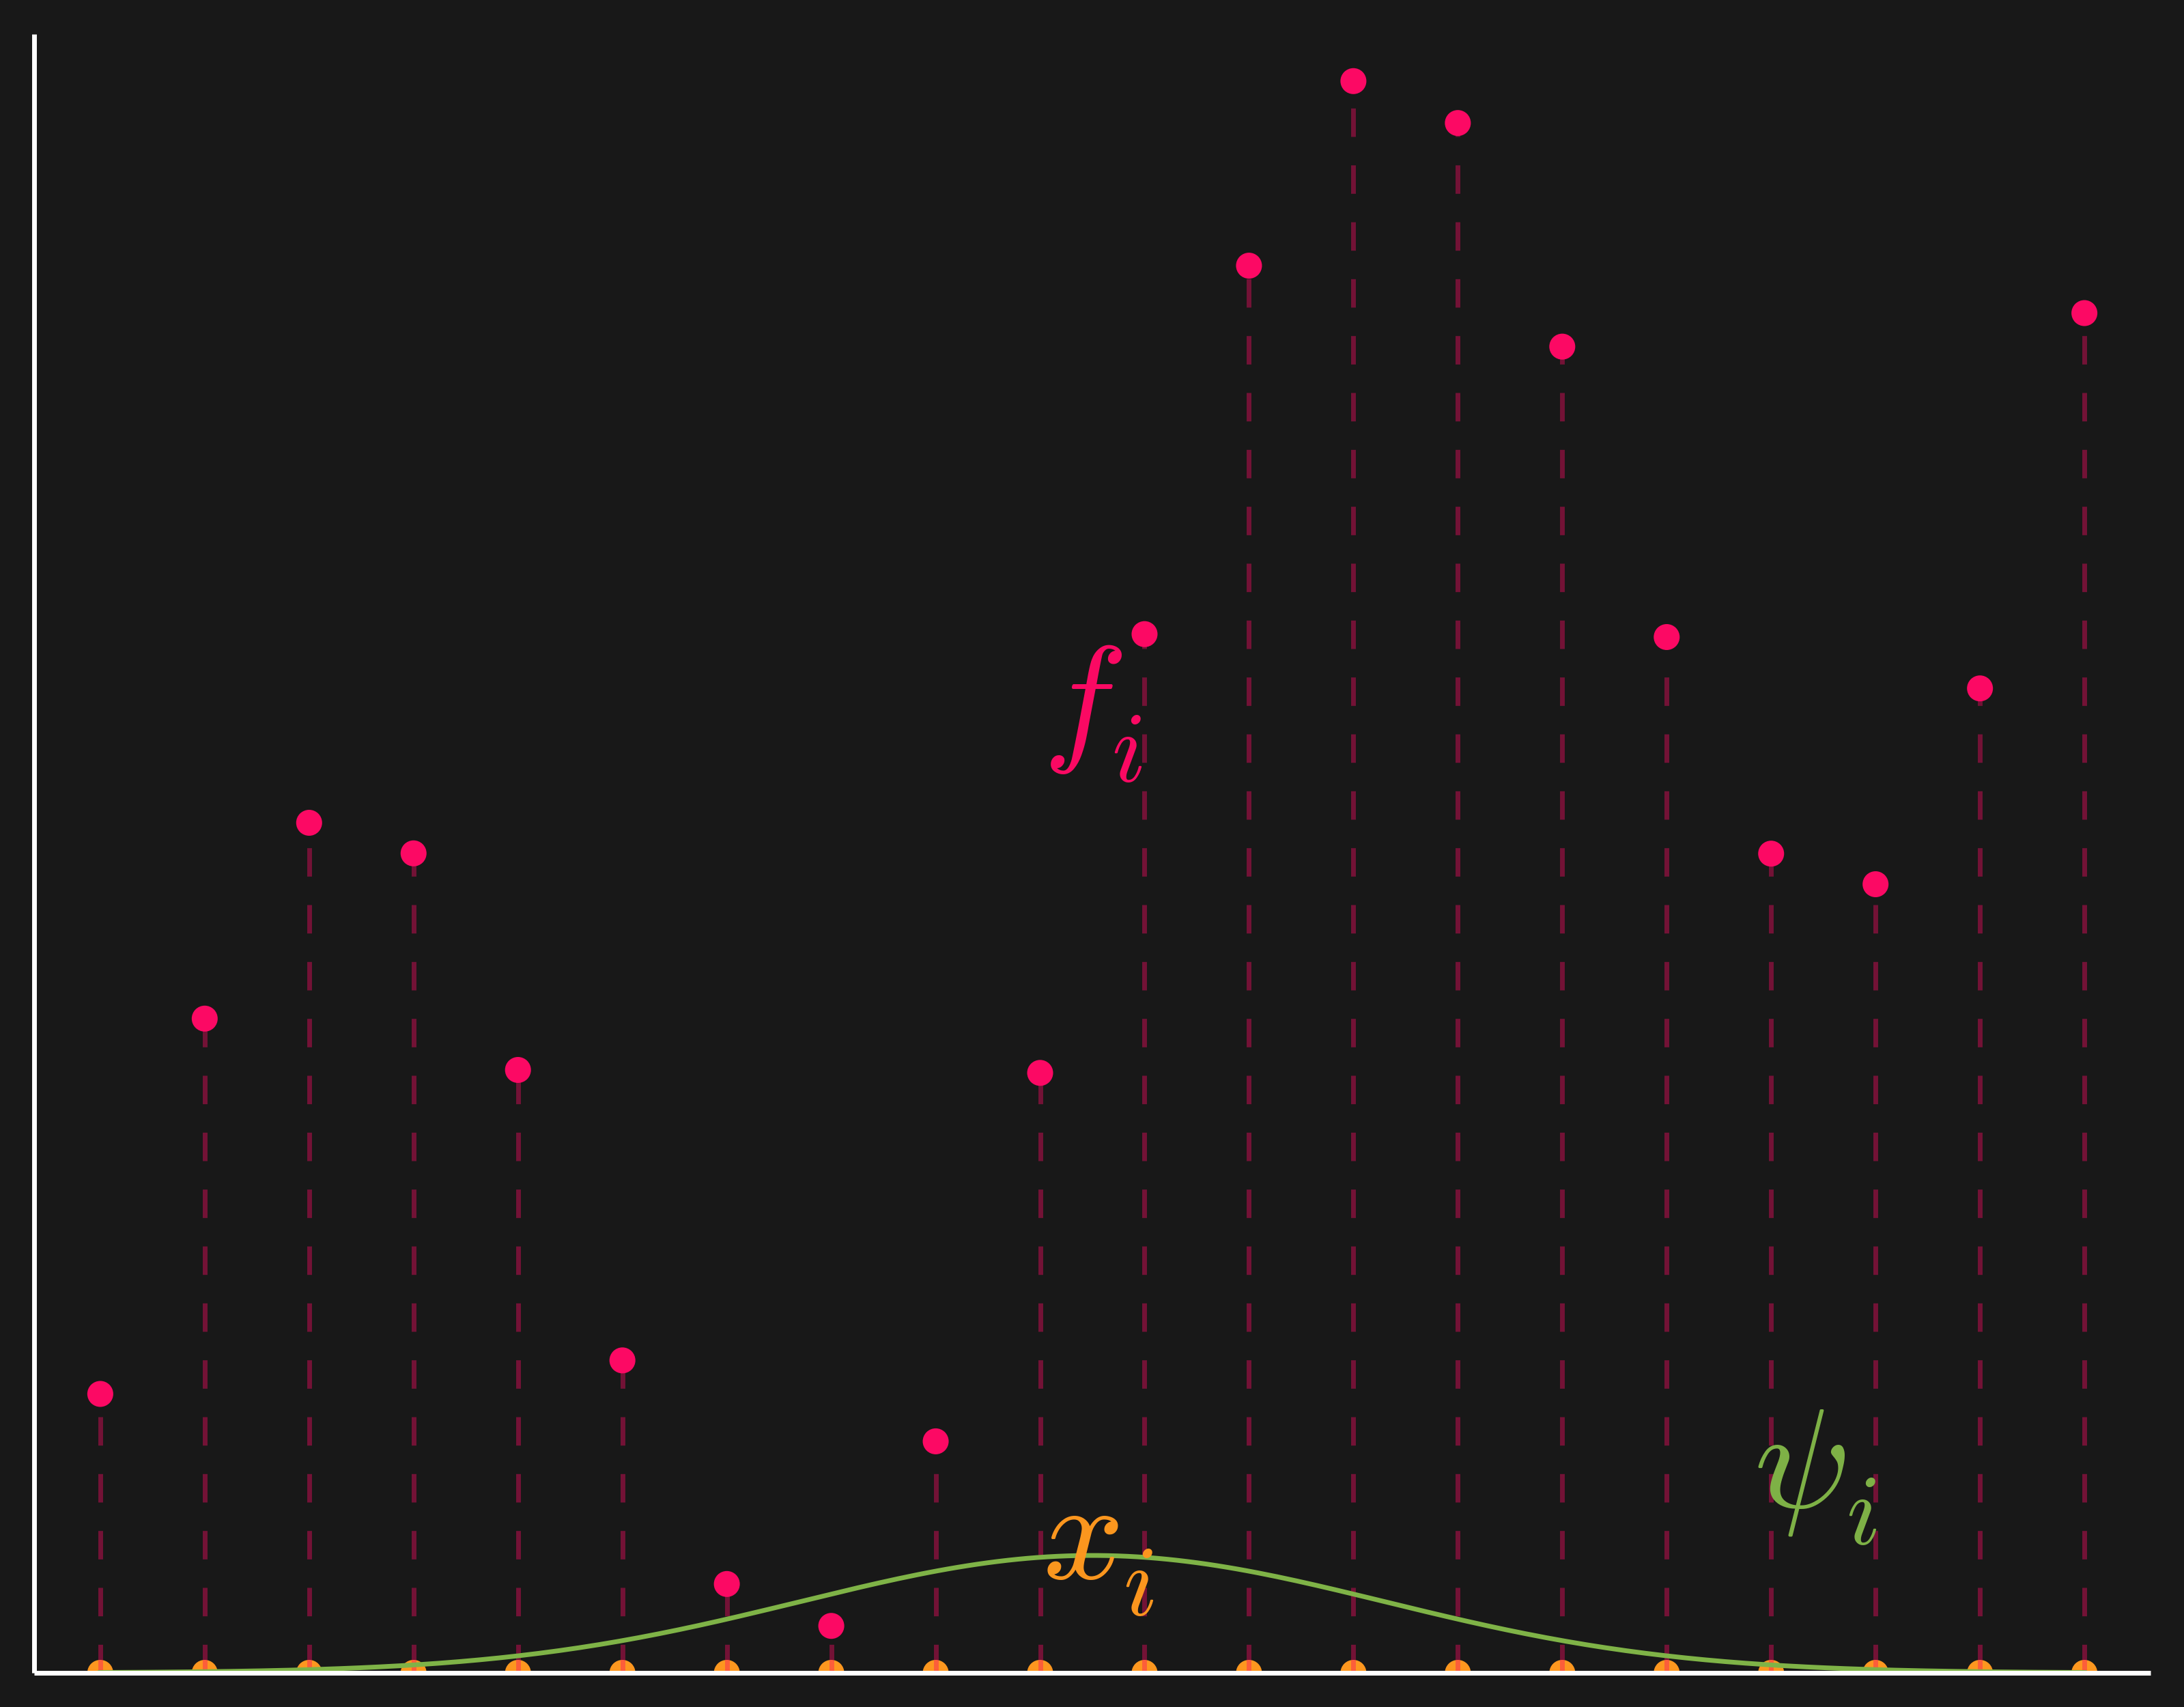
\includegraphics[width=0.9\textwidth, keepaspectratio]{basisgaus1.png}
\end{figure}


\note{}
\end{frame}

\begin{frame}{Visualizing the RBF Method}

\begin{figure}
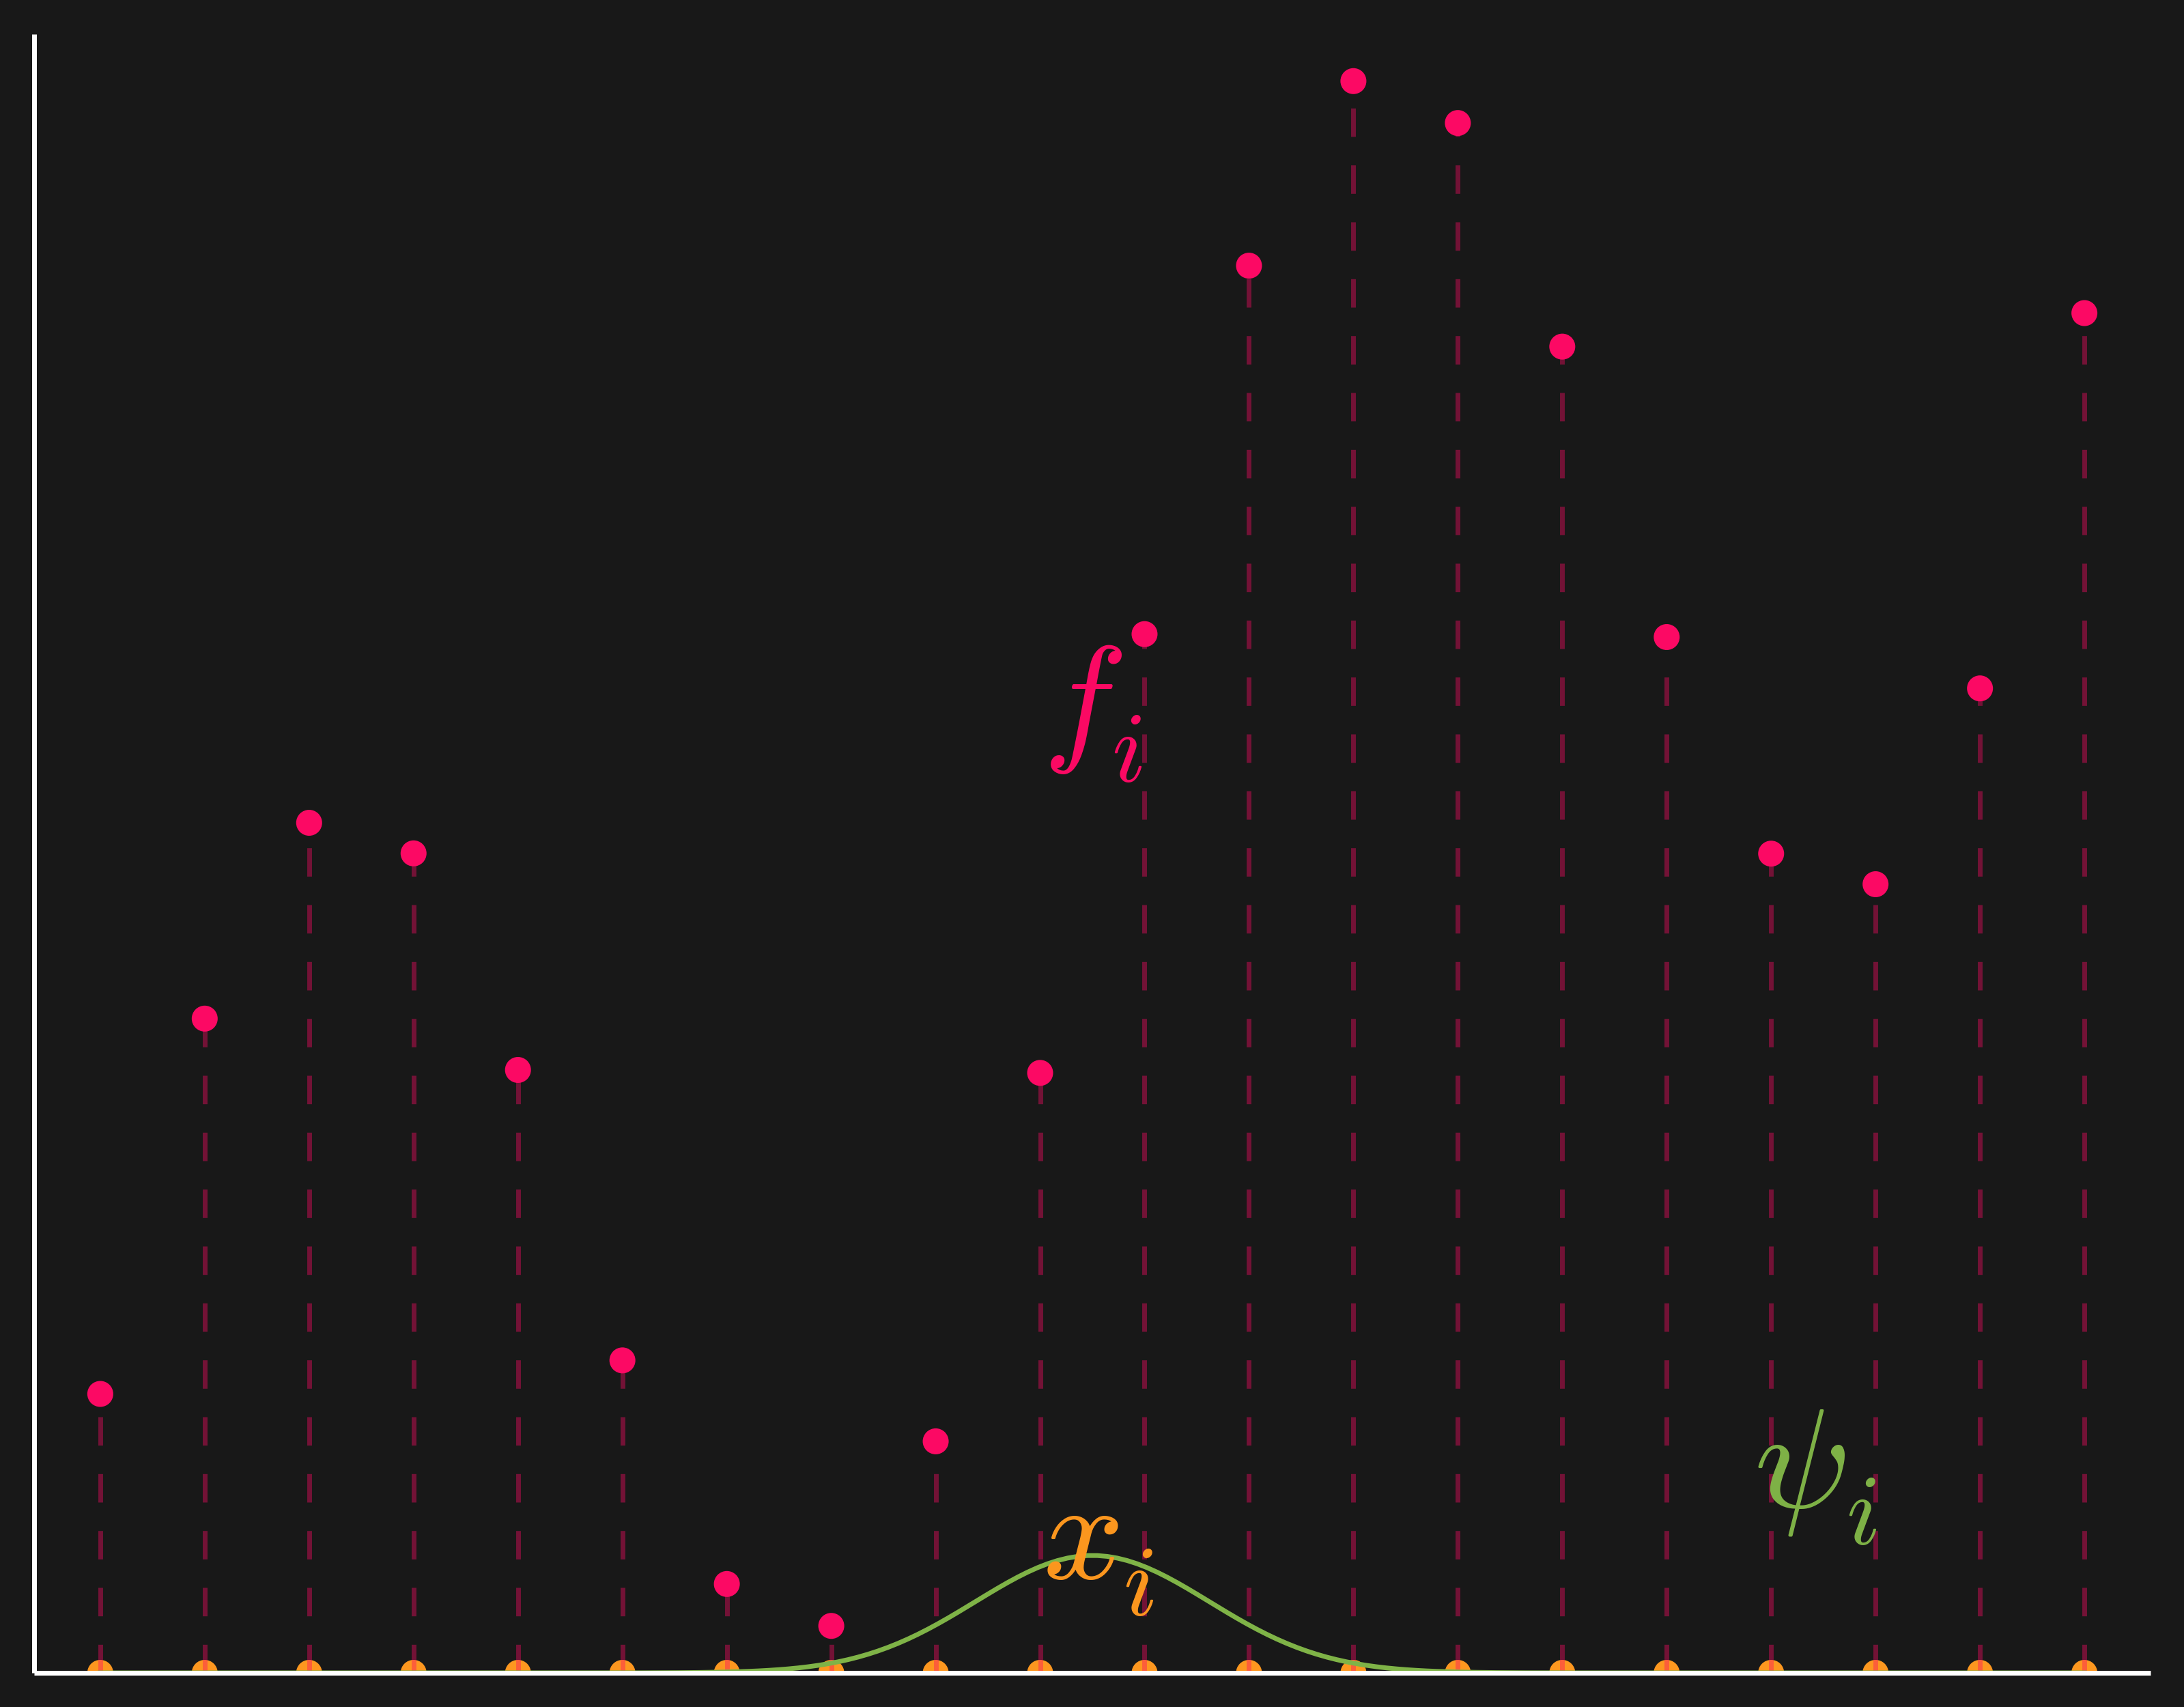
\includegraphics[width=0.9\textwidth, keepaspectratio]{basisgaus2.png}
\end{figure}


\note{}
\end{frame}

\begin{frame}{Well-Posed $\neq$ Well-Conditioned}
We now know that our system is well-posed, so a unique solution exists.

\bigskip

However, this solution isn't always accessible using numerical methods, making it \subt{ill-conditioned} due to a loss of precision in computationally solving the linear system.

\bigskip

Radial Basis Interpolation has the propensity to be ill-conditioned, especially when choosing shape parameter, $\epsilon$.



\note{}
\end{frame}

\begin{frame}{Pure Mathematicians can Leave Now}

\begin{figure}
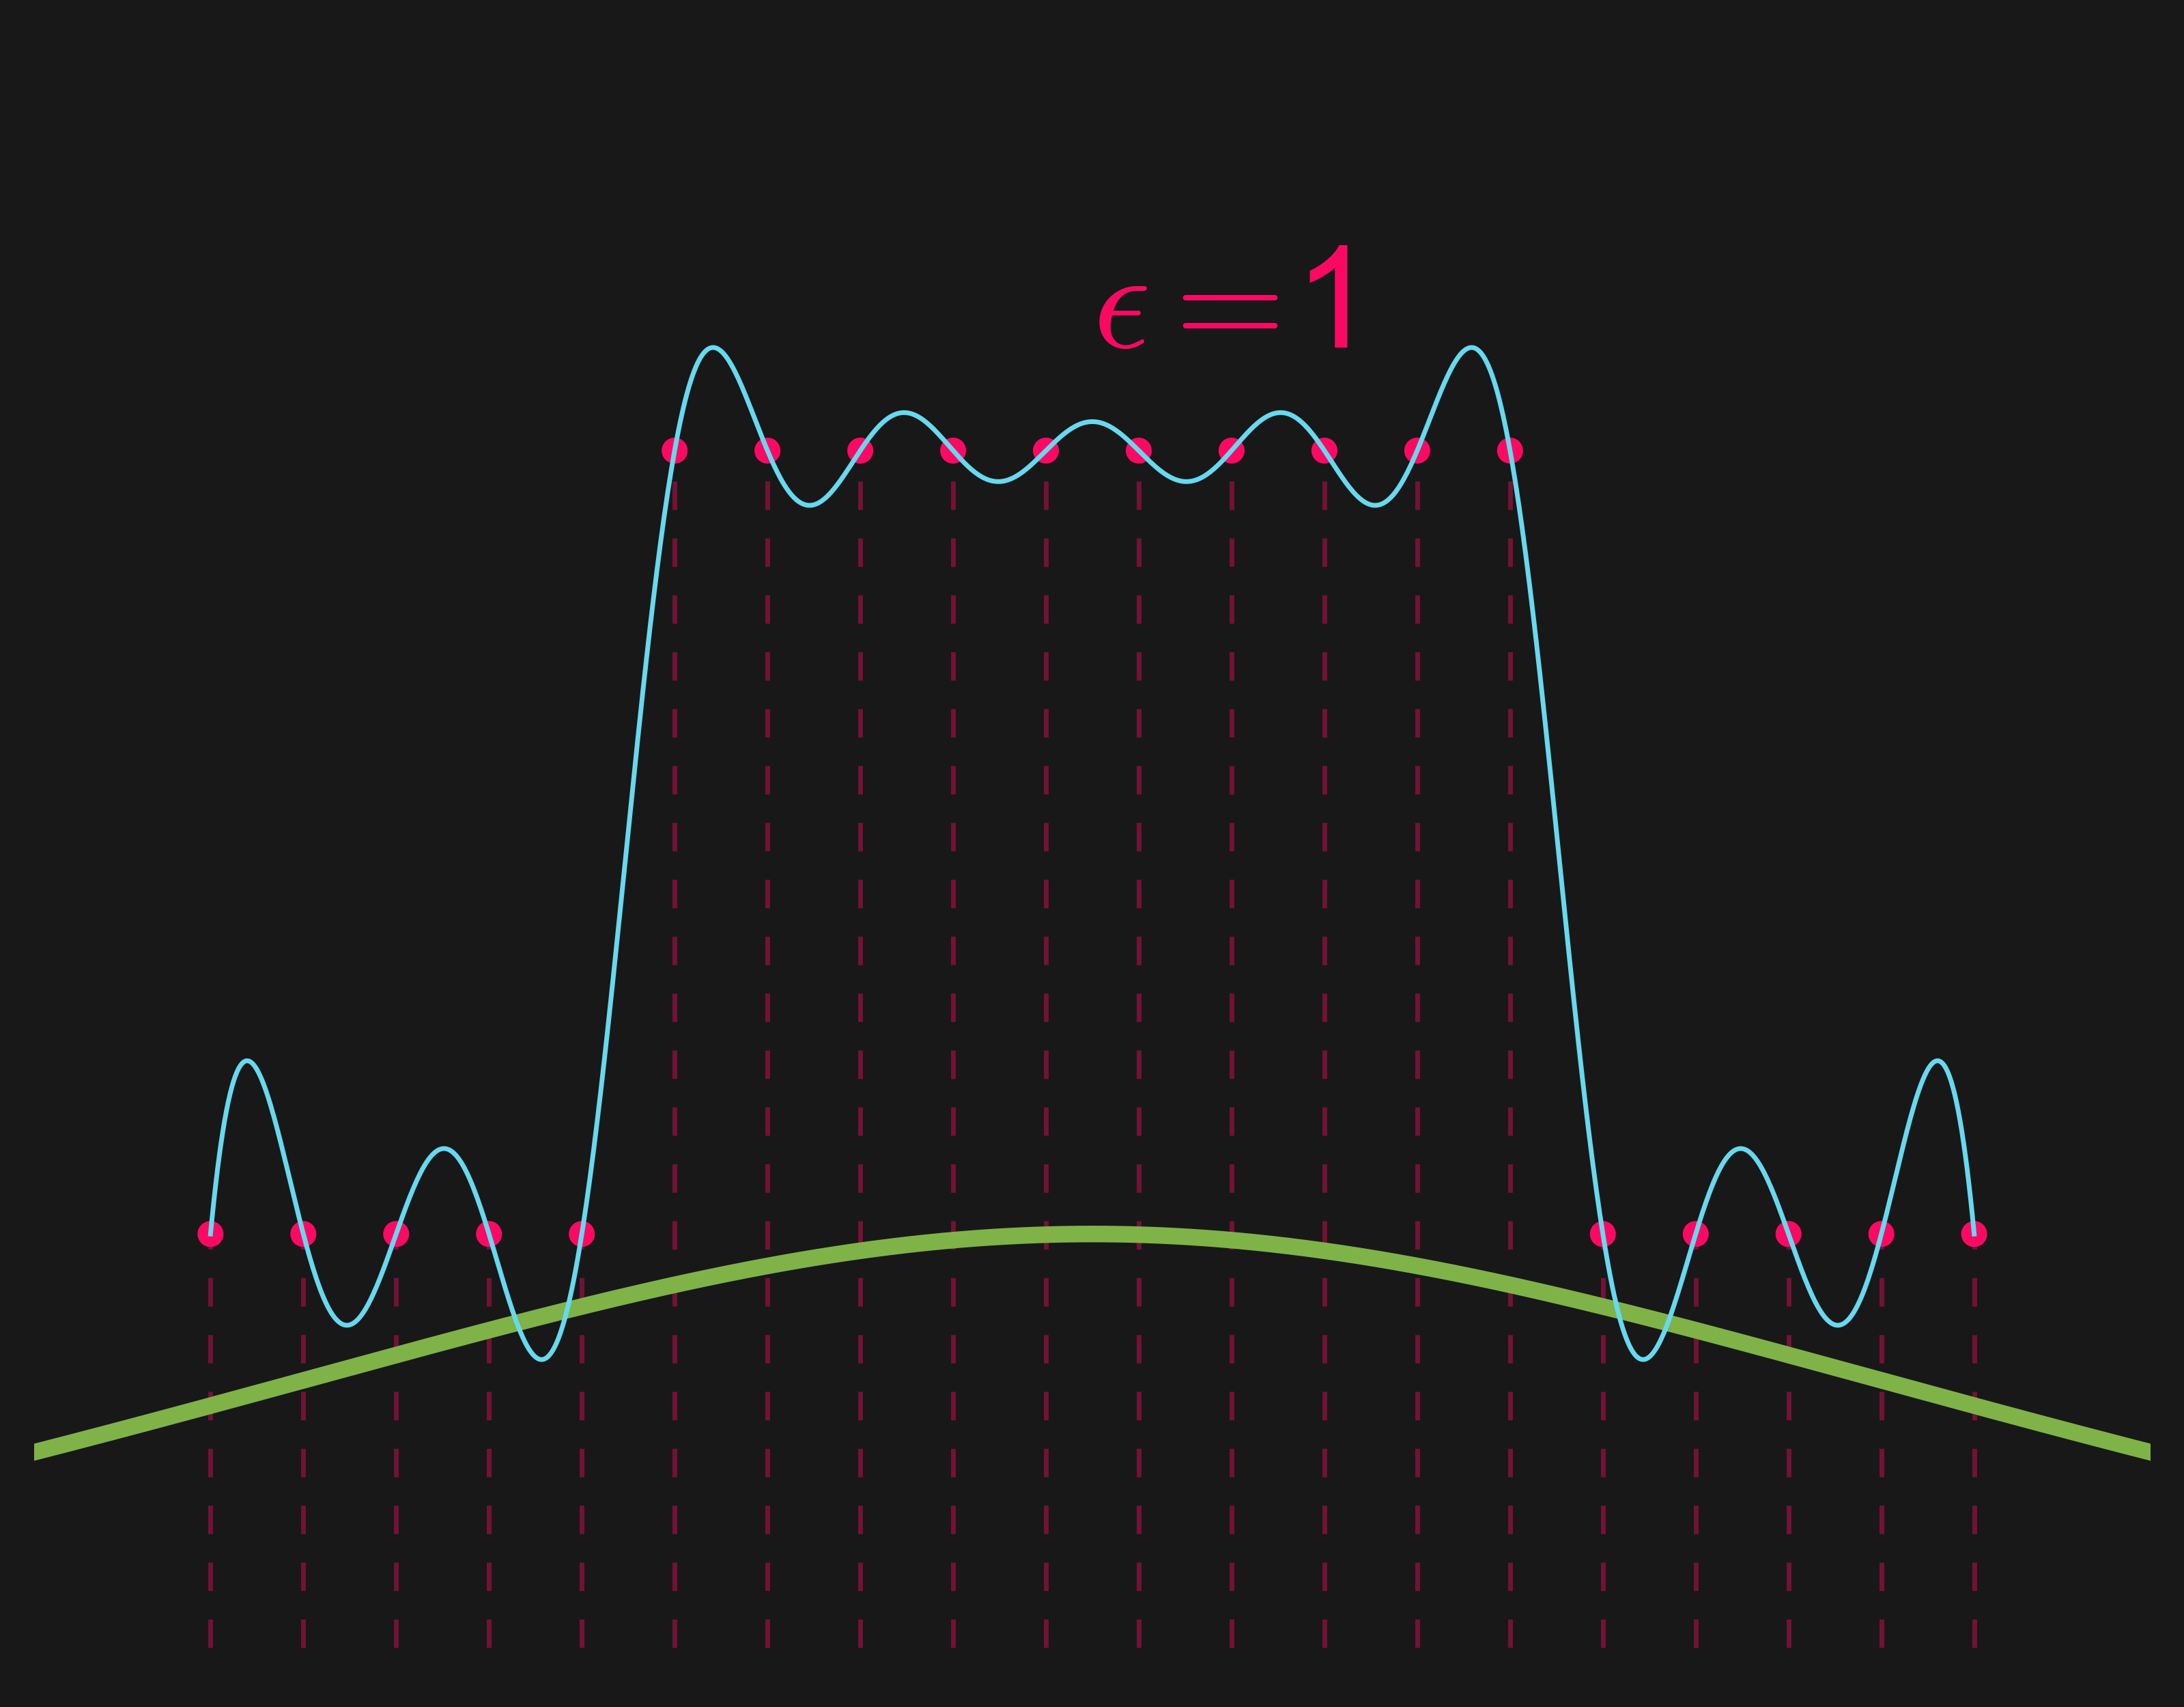
\includegraphics[width=0.9\textwidth, keepaspectratio]{conditioned.png}
\end{figure}


\note{}
\end{frame}

\begin{frame}{Pure Mathematicians can Leave Now}

\begin{figure}
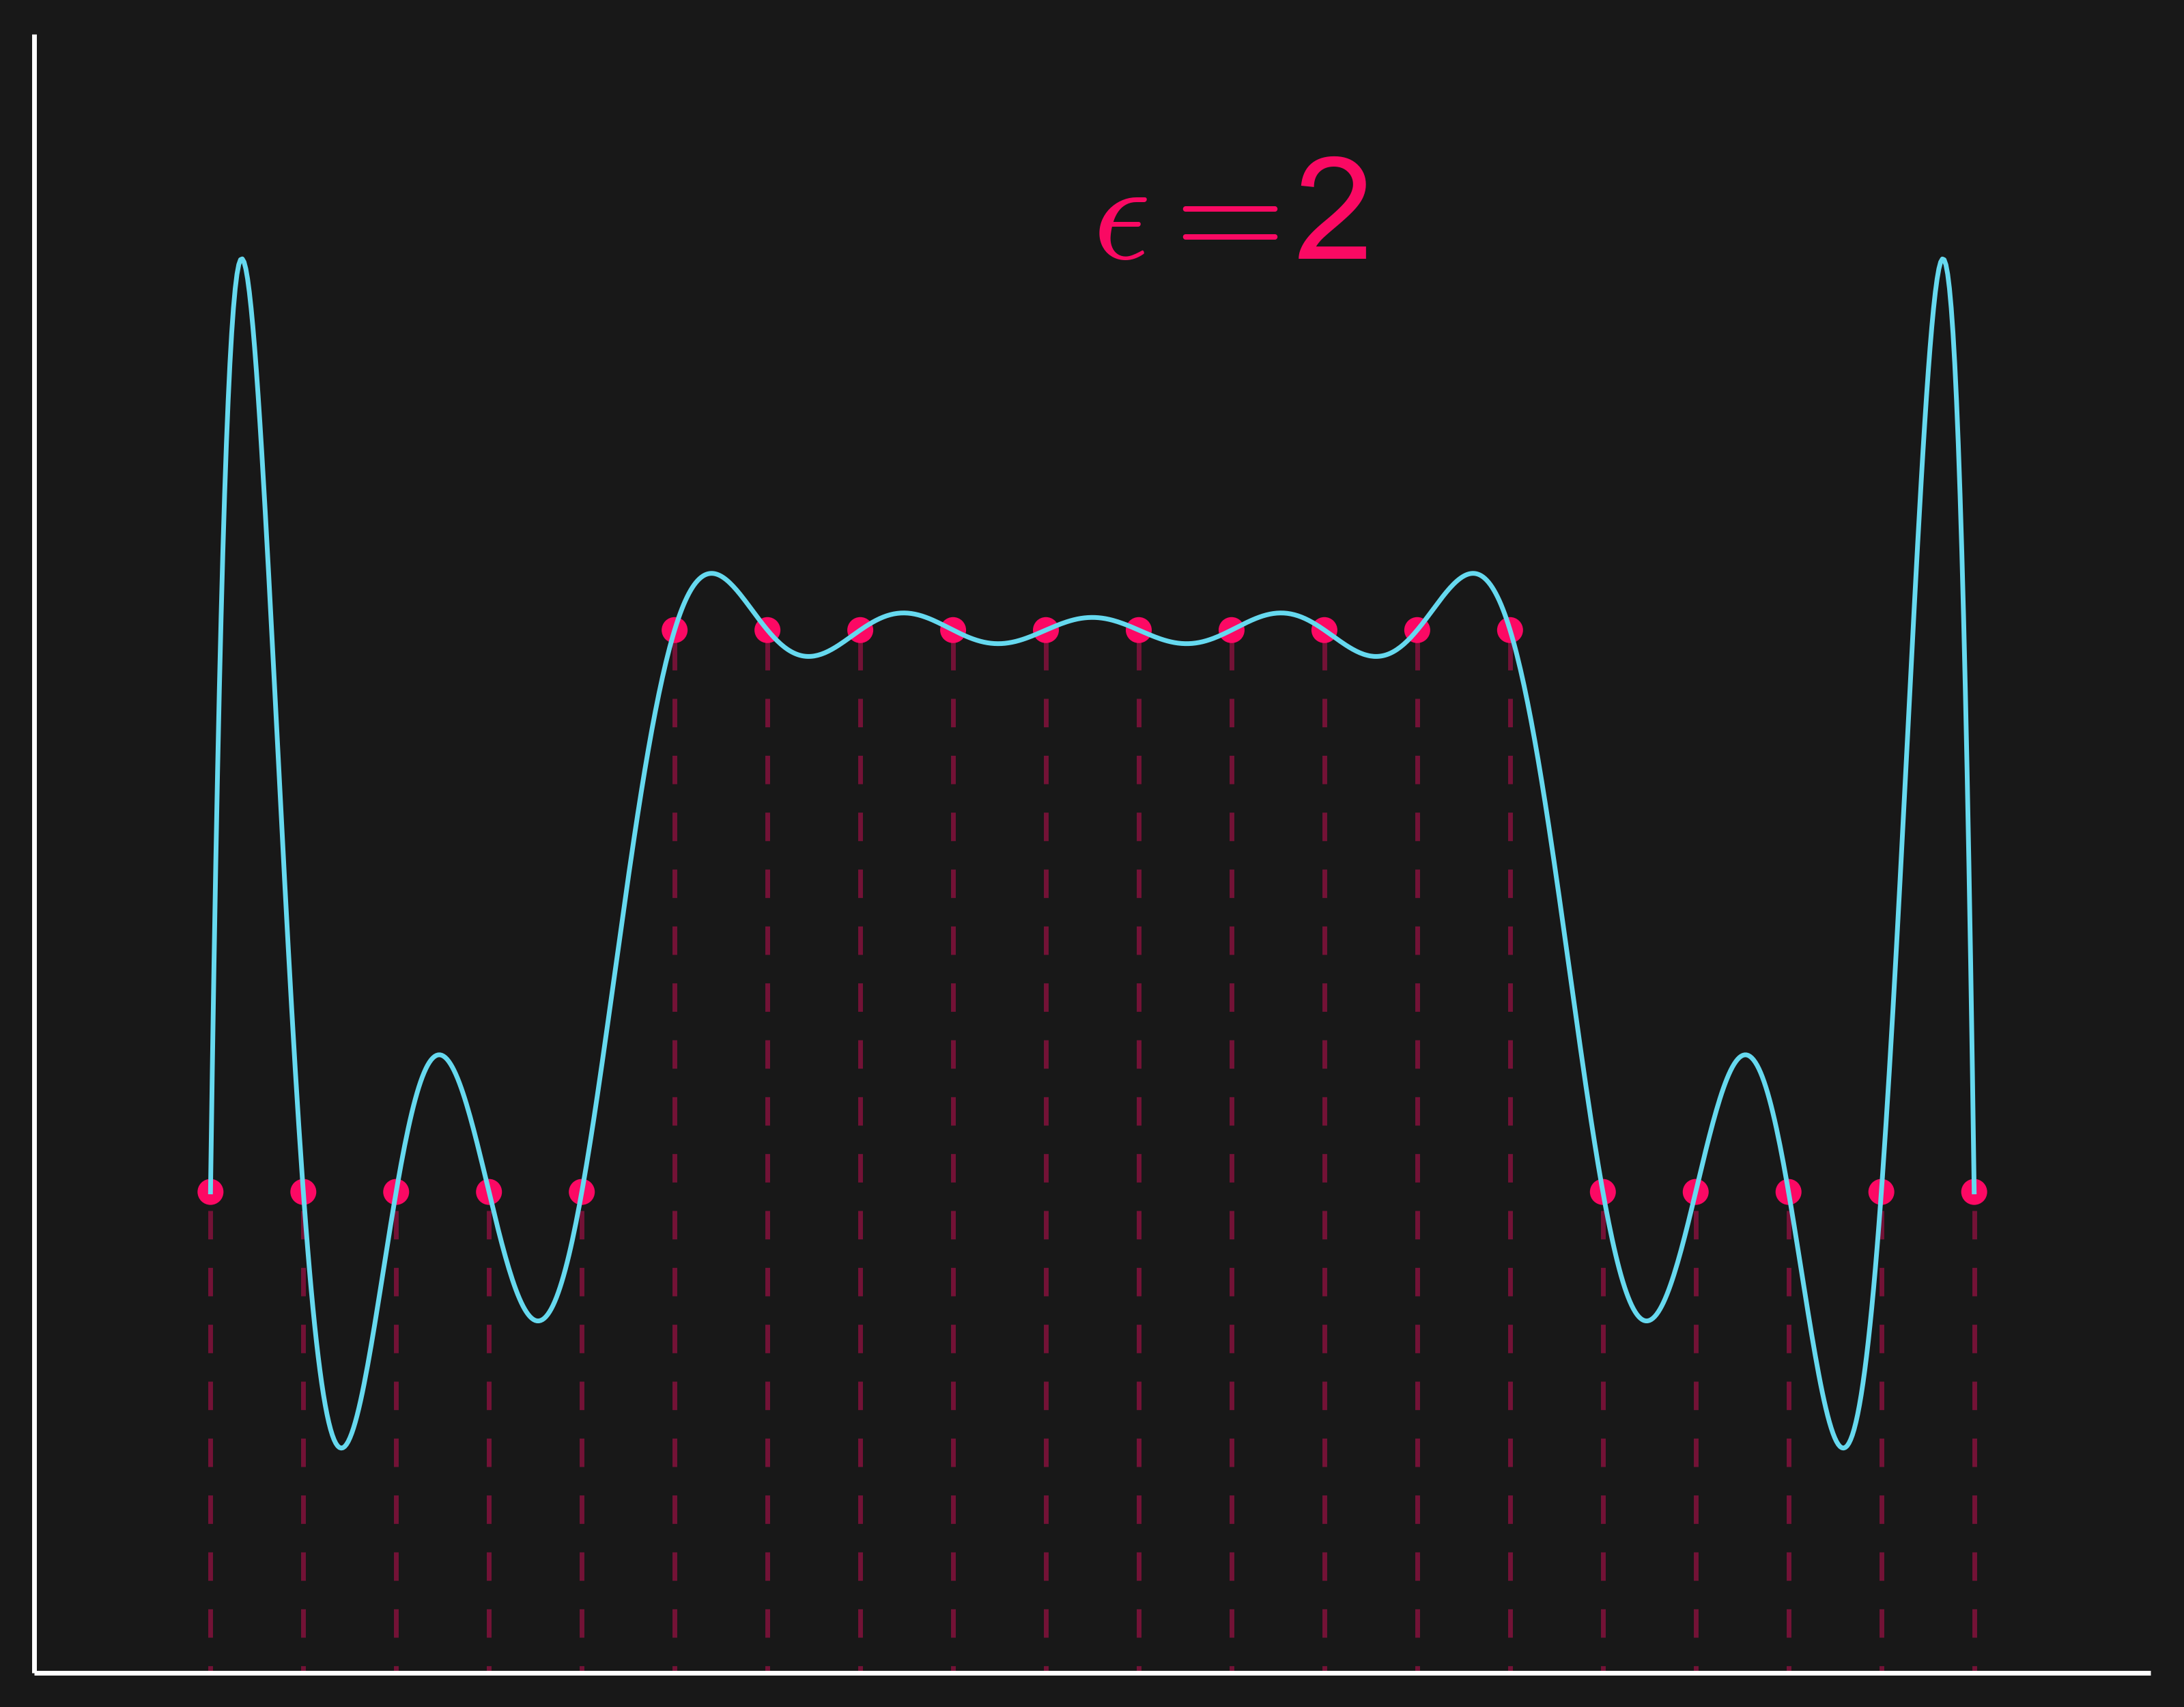
\includegraphics[width=0.9\textwidth, keepaspectratio]{illconditioned.png}
\end{figure}


\note{}
\end{frame}

\begin{frame}{Pure Mathematicians can Laugh Now}

\begin{figure}
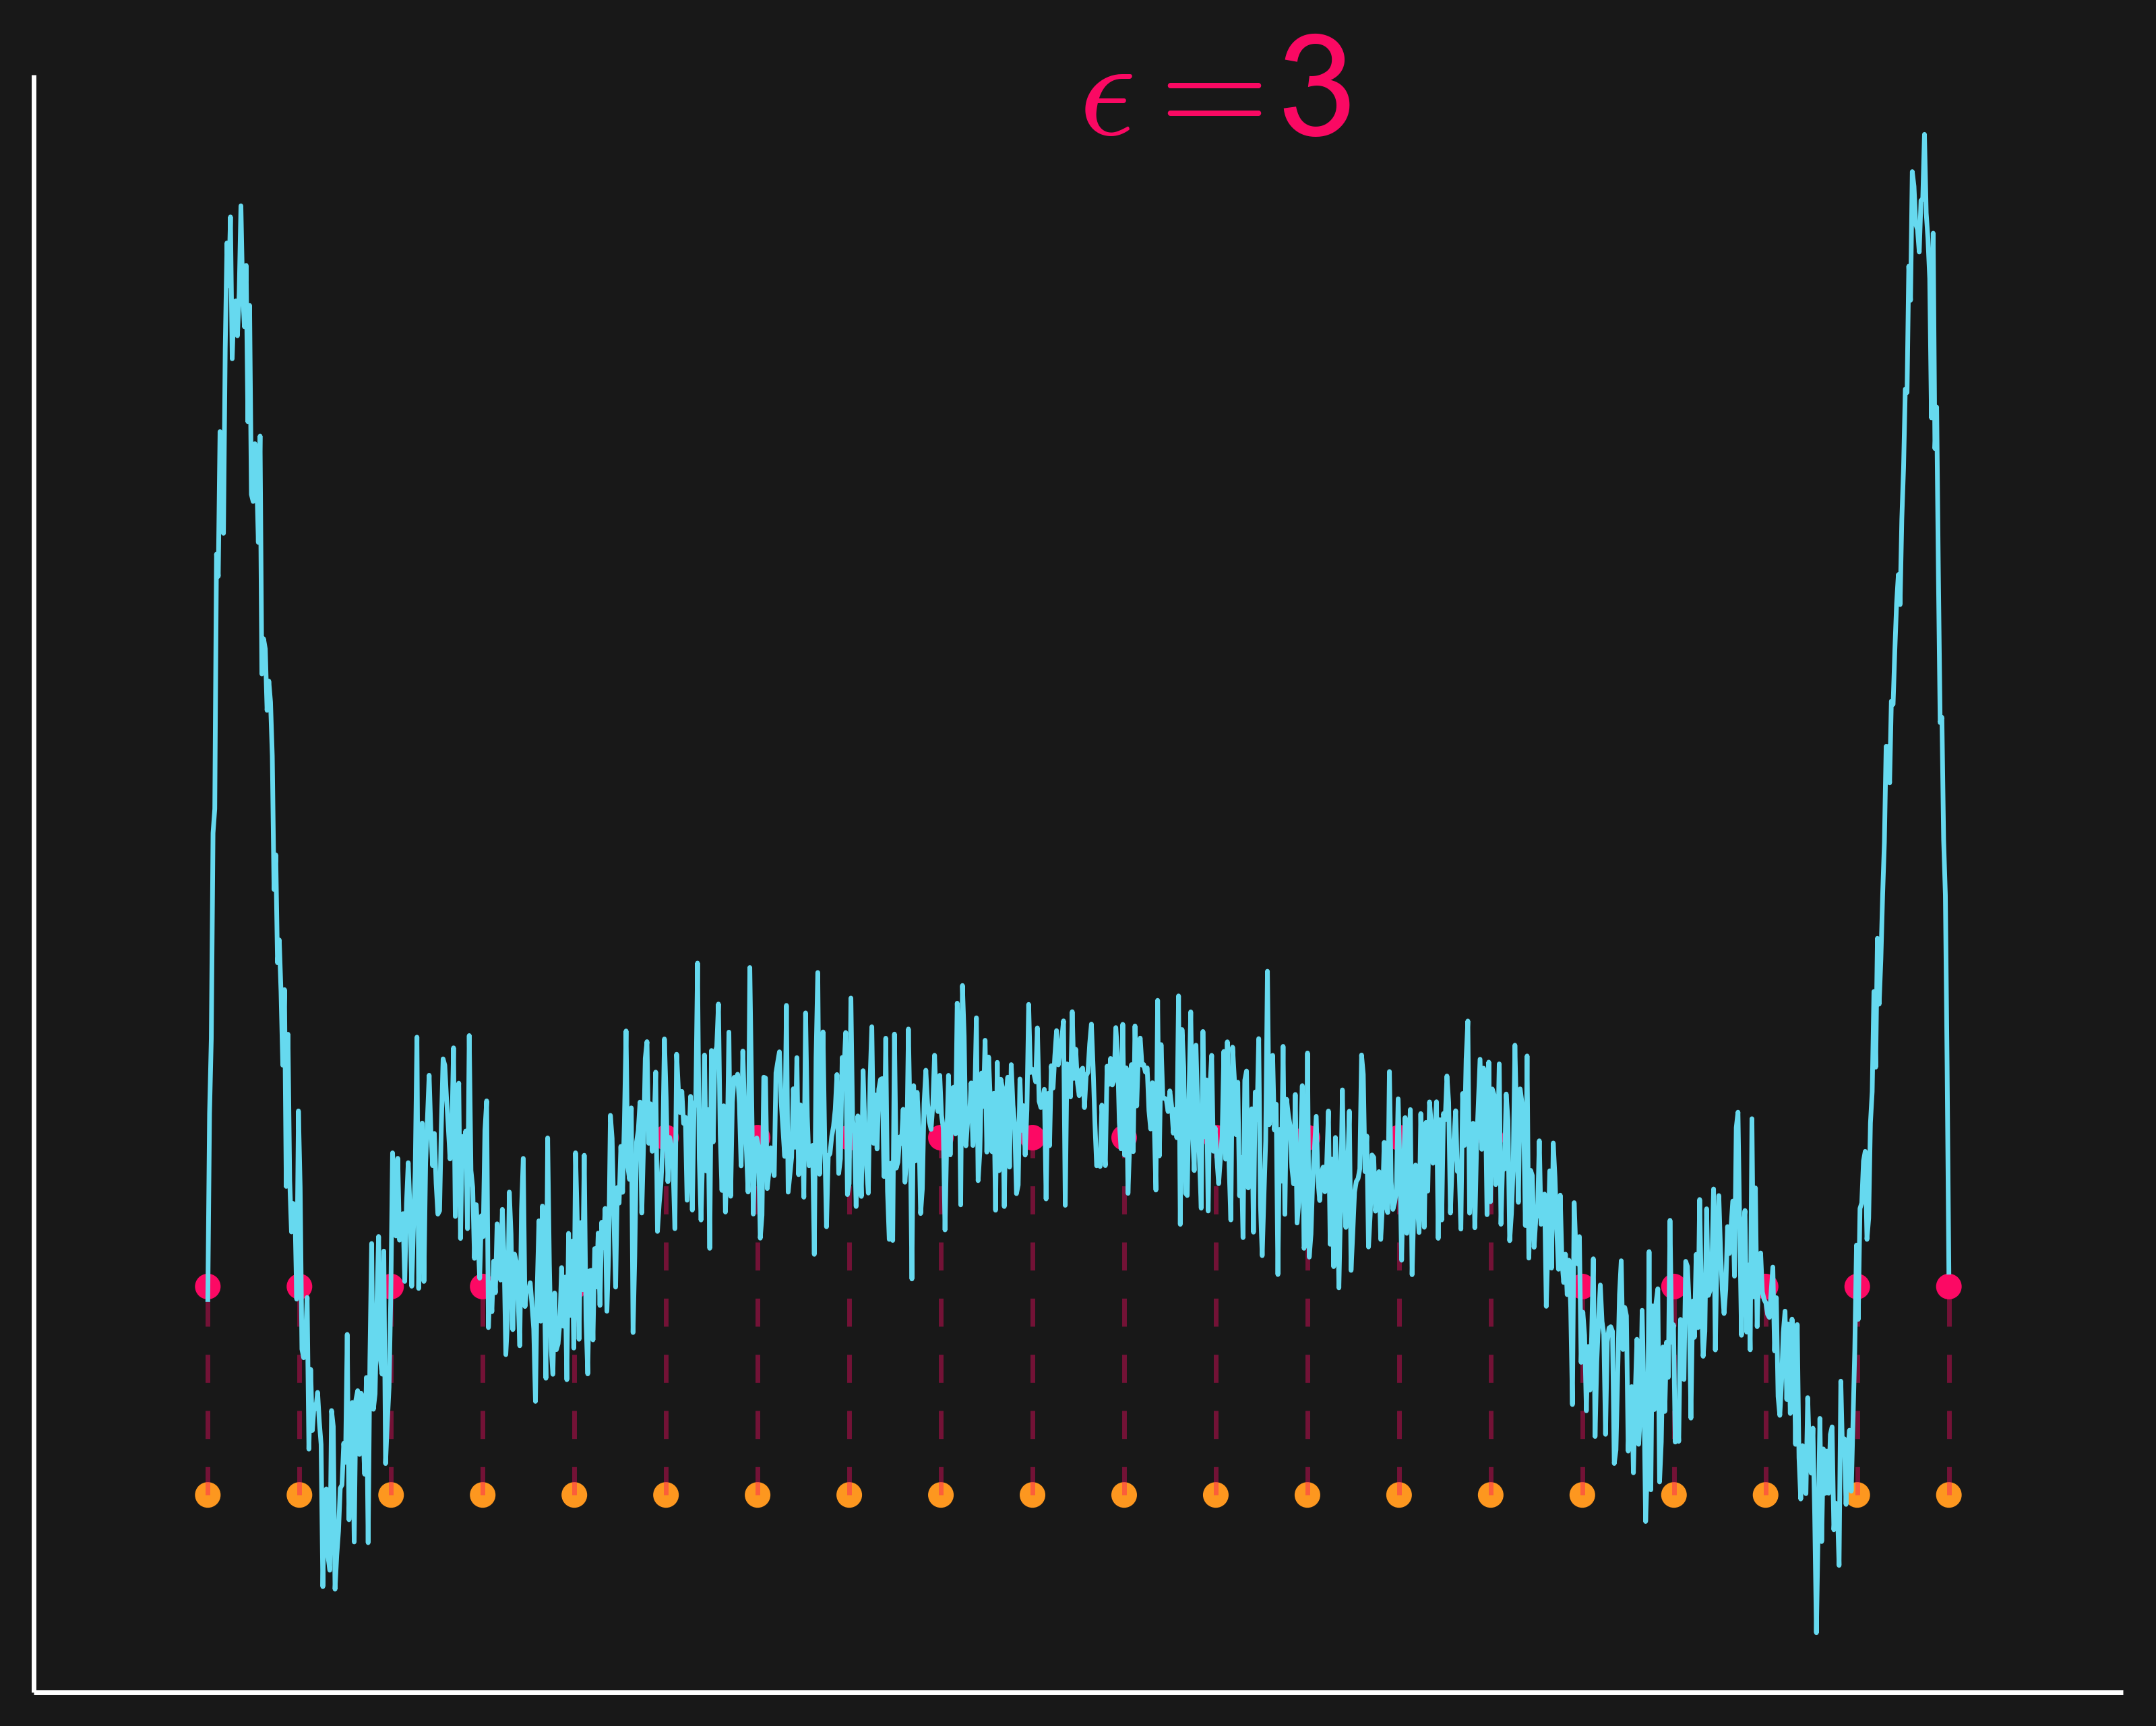
\includegraphics[width=0.9\textwidth, keepaspectratio]{veryillconditioned.png}
\end{figure}


\note{}
\end{frame}

\begin{frame}{Considerations When Using RBFs}
\bi
\item The interpolation matrix, A, is dense $\implies$ Computationally Expensive
\item Choosing shape parameter, $\epsilon$, often involves optimization
\item RBF interpolation can easily be ill-conditioned
\item Interpolation error blows up near boundaries
\ei

\begin{figure}[!htb]
\minipage{0.50\textwidth}
  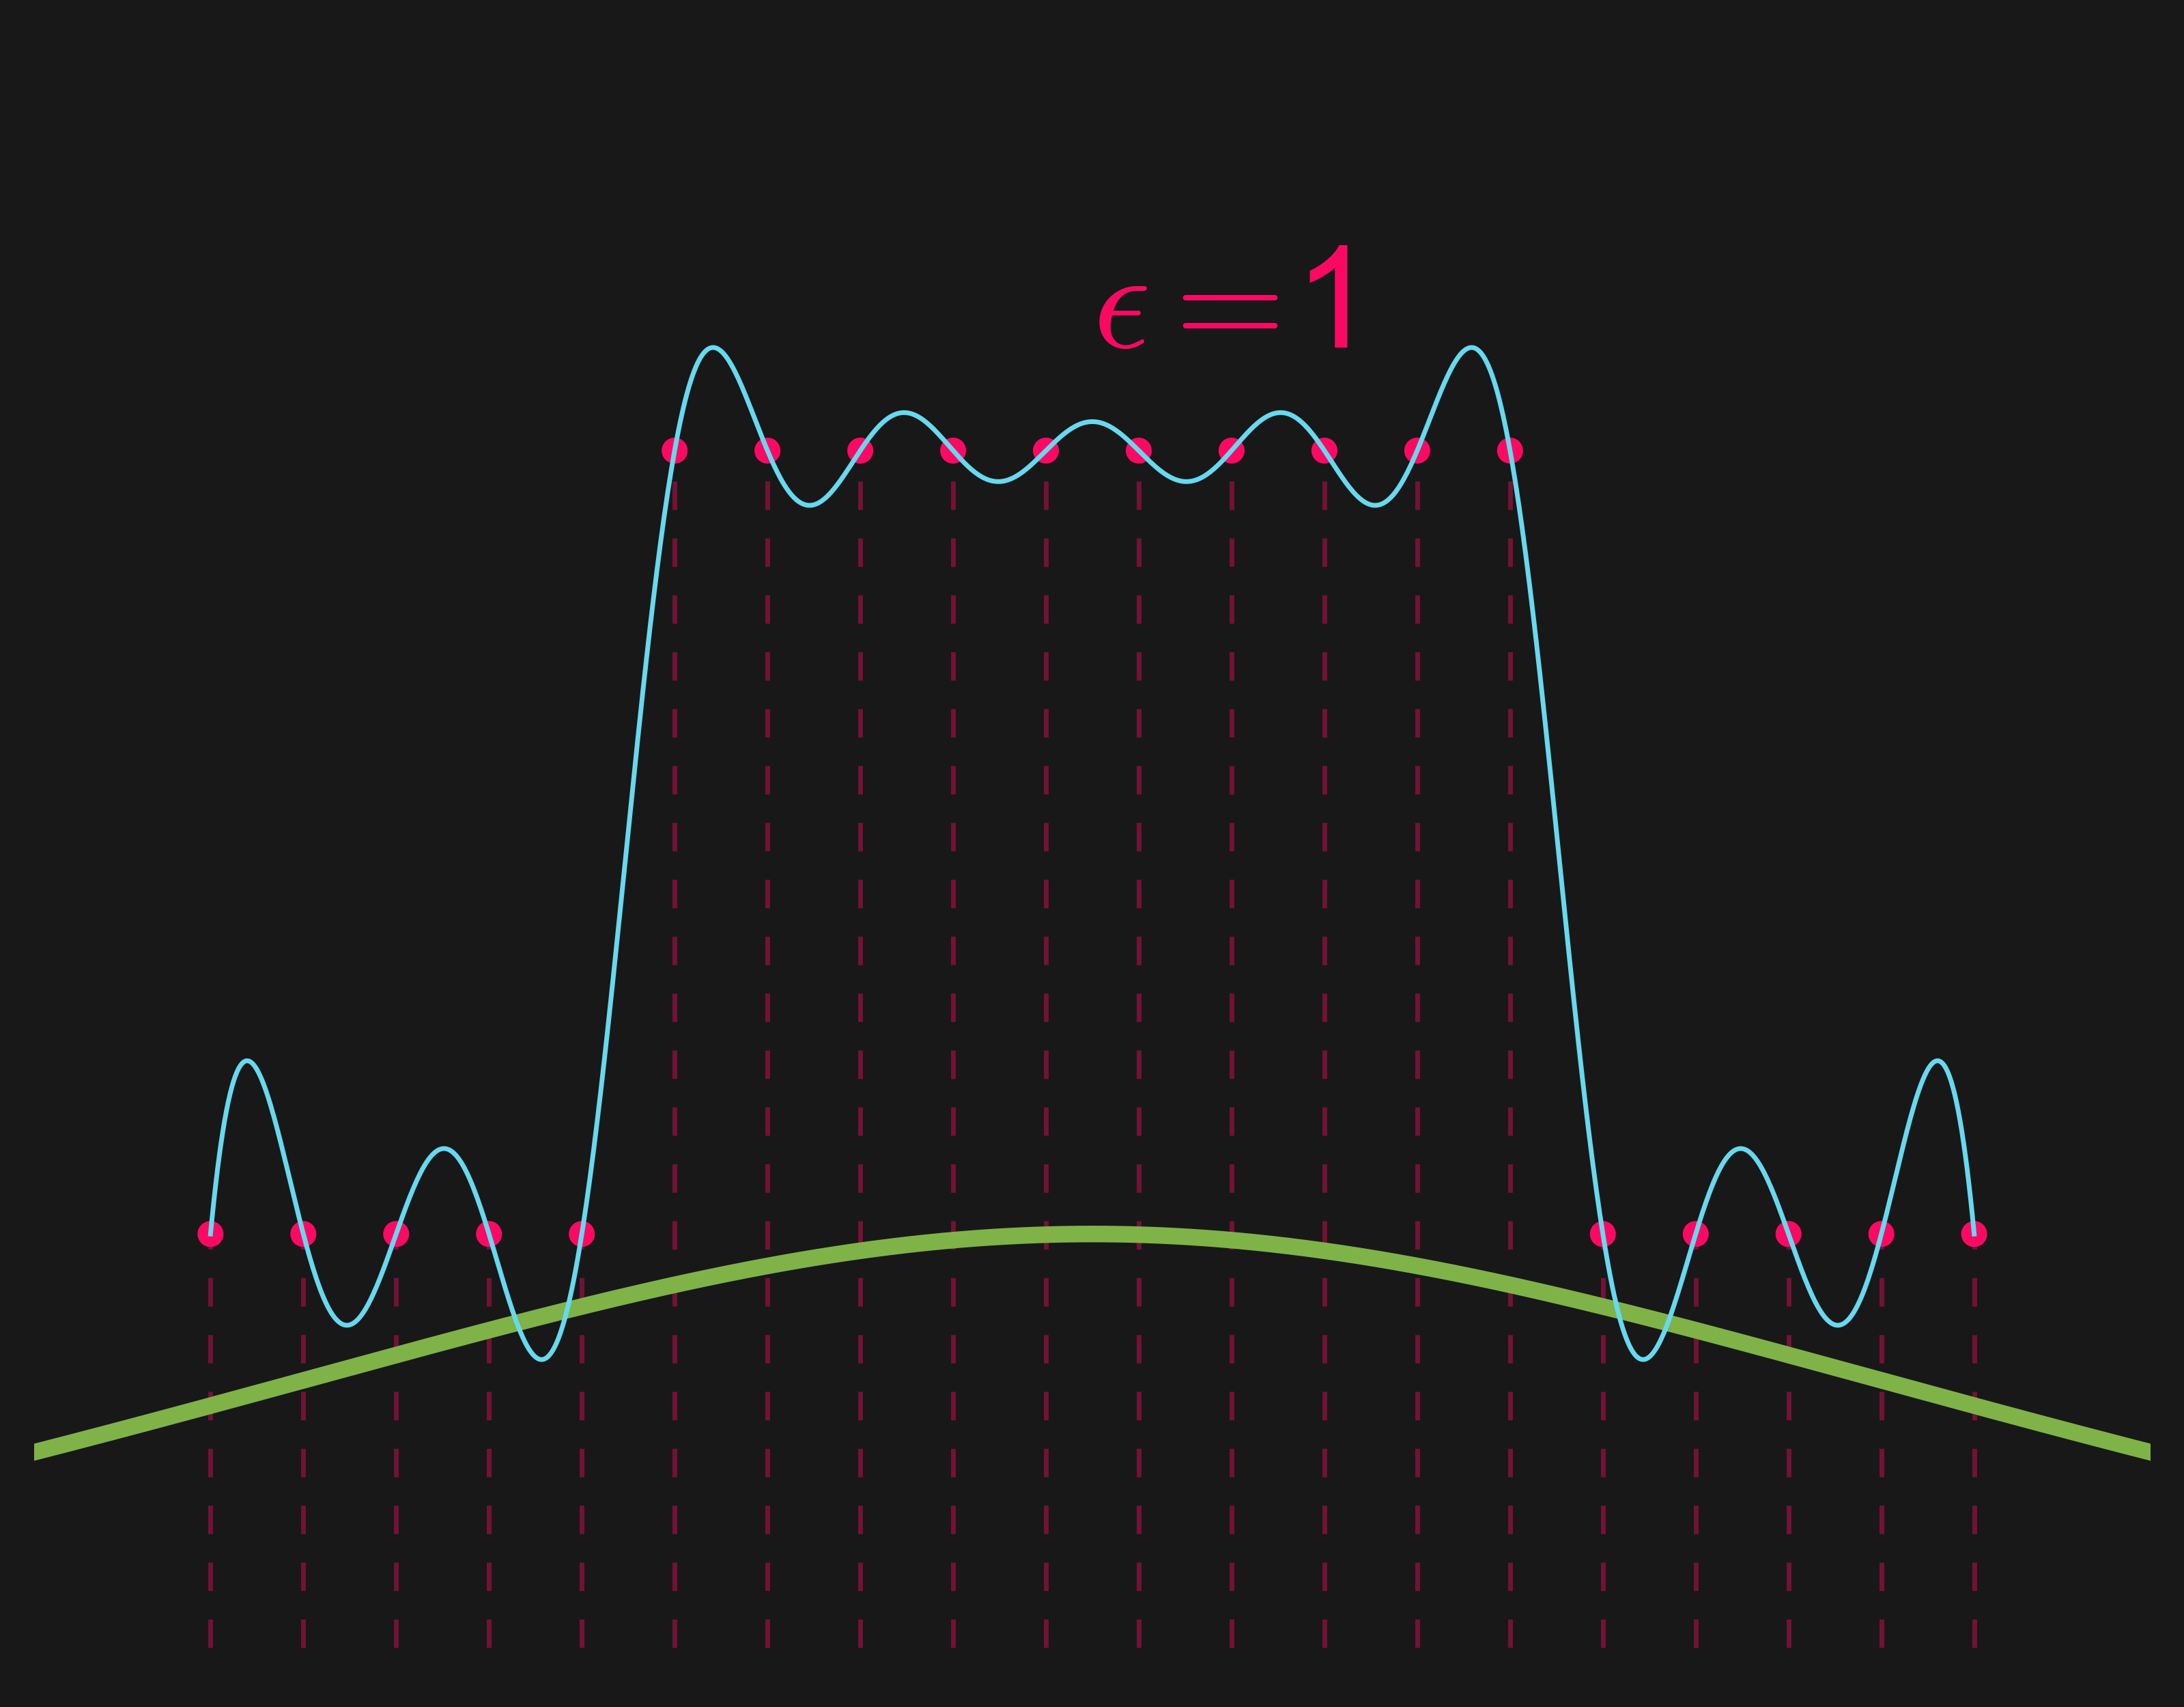
\includegraphics[width=\linewidth]{conditioned.png}
\endminipage\hfill
\minipage{0.50\textwidth}
  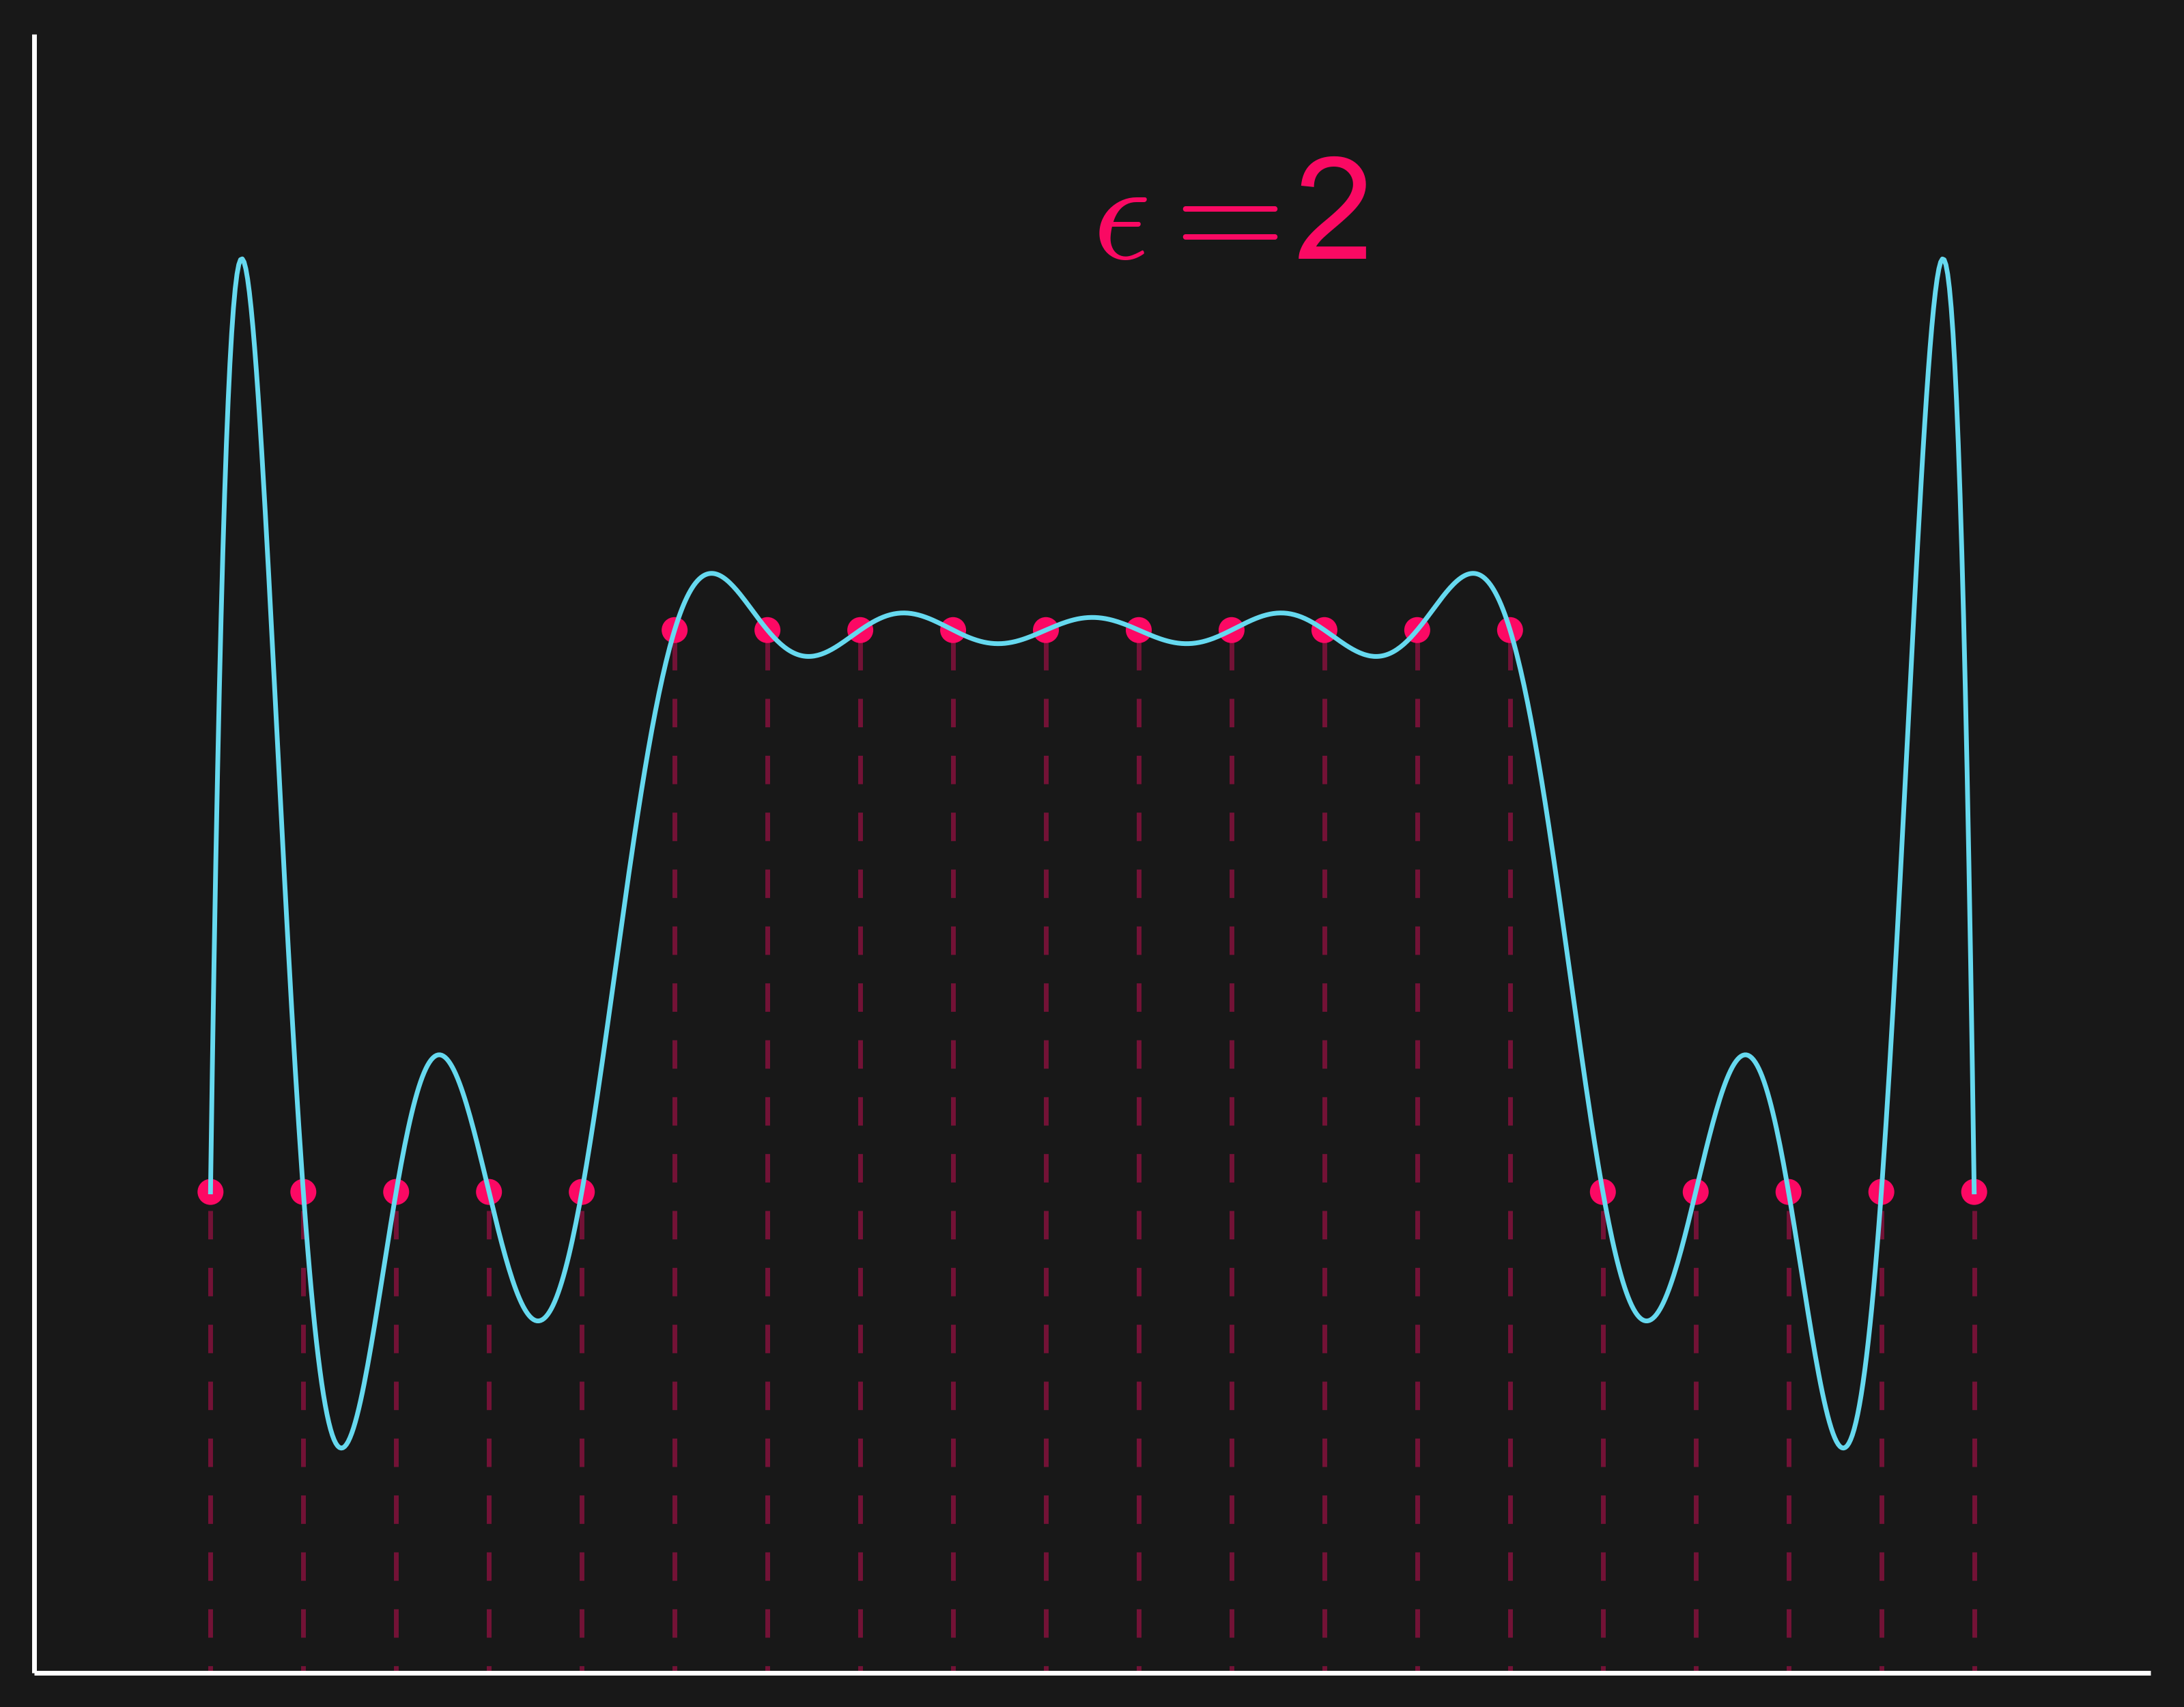
\includegraphics[width=\linewidth]{illconditioned.png}
\endminipage\
\end{figure}

\note{}
\end{frame}

\begin{frame}{Considerations When Using RBFs}
\subt{Interpolation error blows up near bounderies}

Why? Because our basis functions are centered at our data and kernels will be asymmetric near boundaries.

\begin{figure}[!htb]
\minipage{0.50\textwidth}
  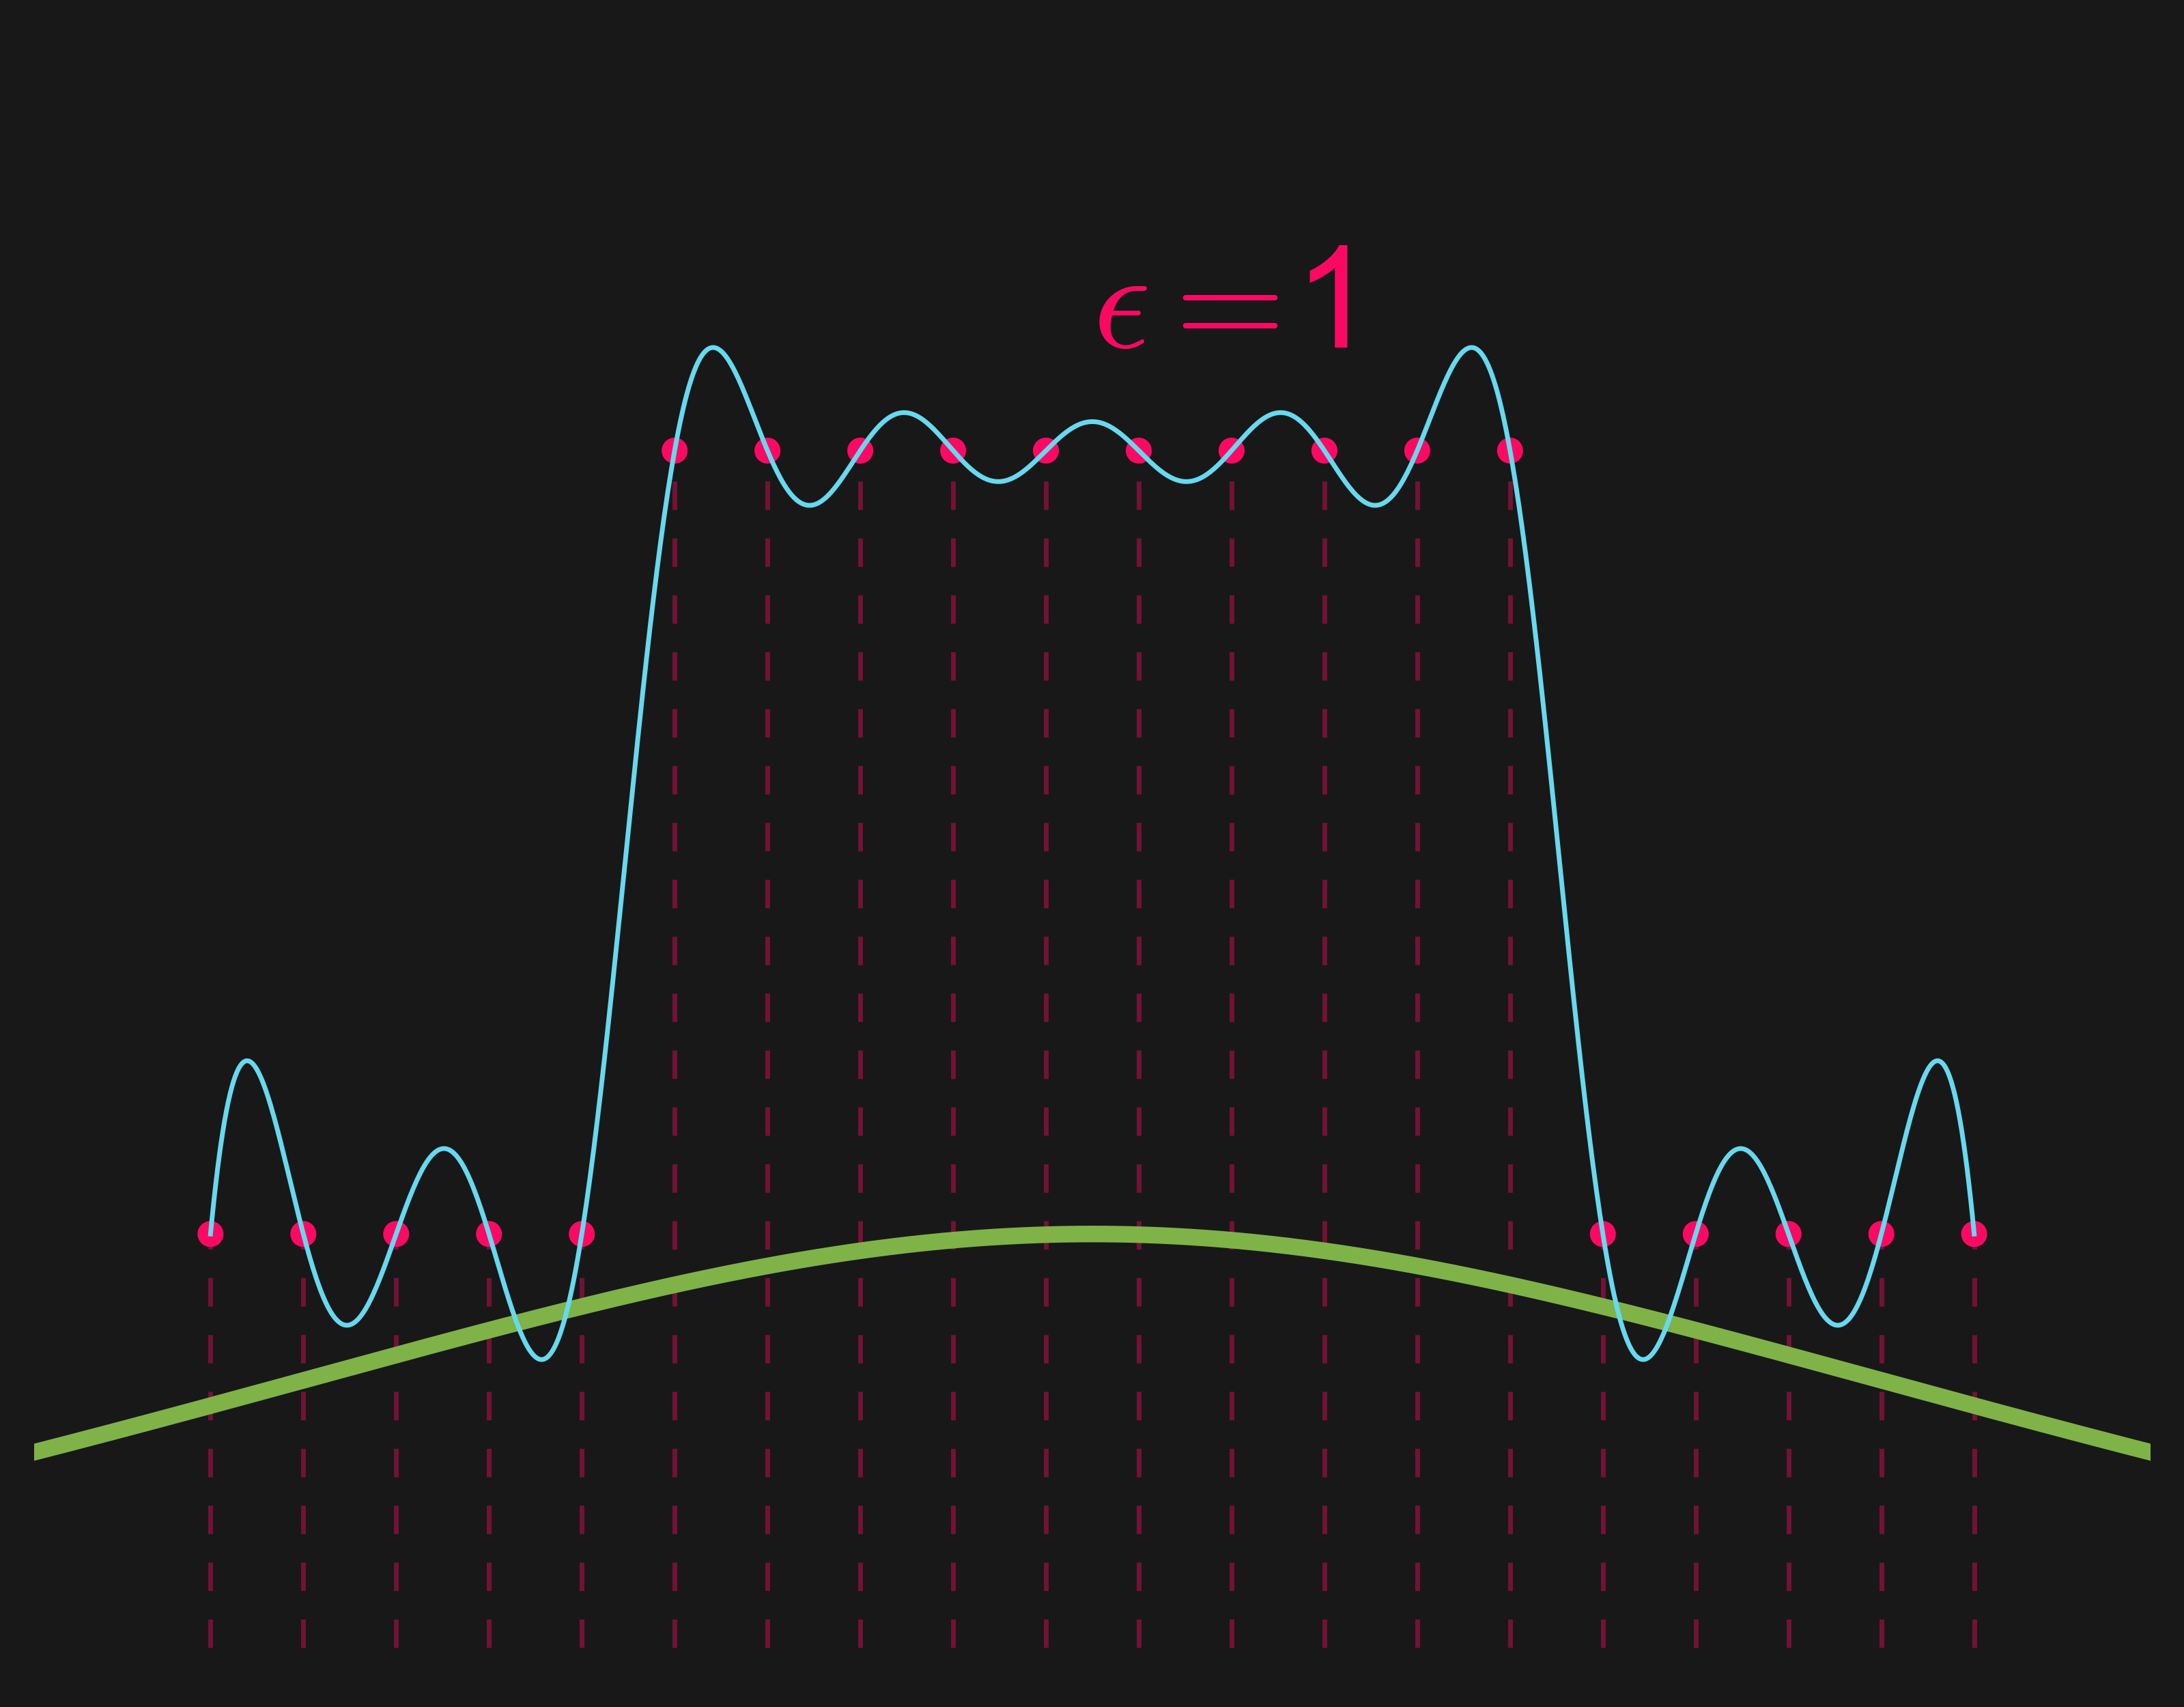
\includegraphics[width=\linewidth]{conditioned.png}
\endminipage\hfill
\minipage{0.50\textwidth}
  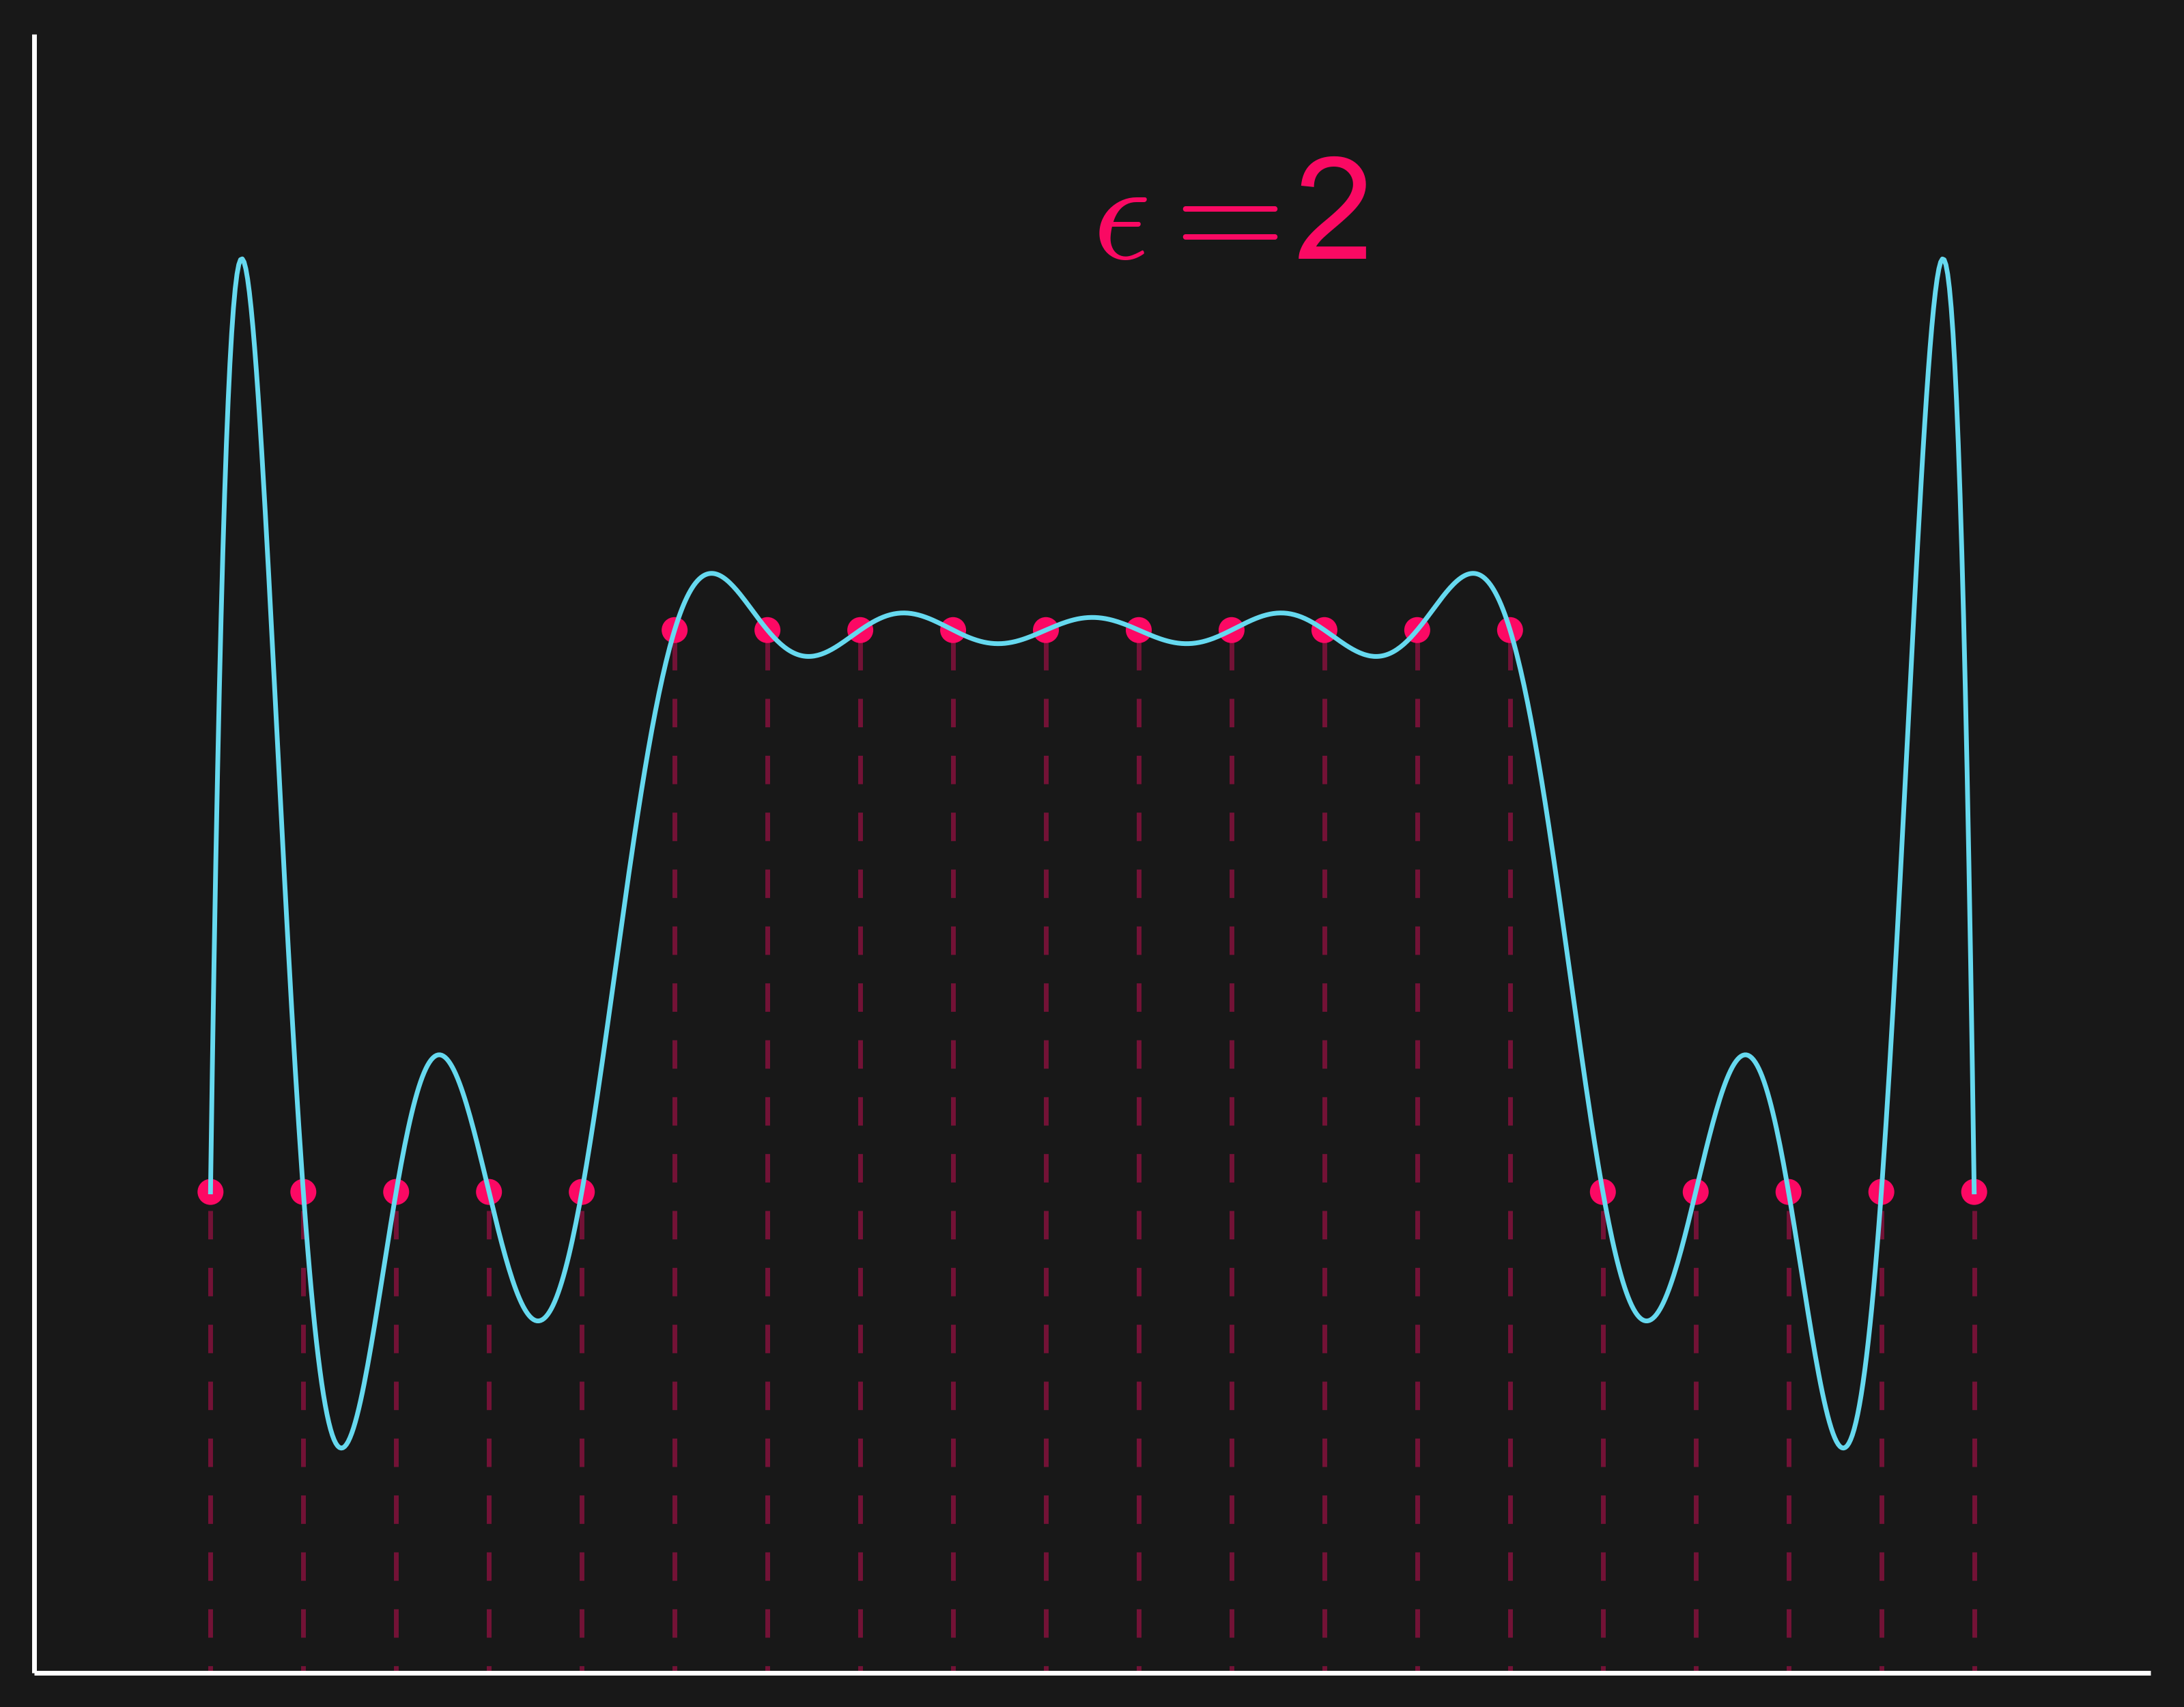
\includegraphics[width=\linewidth]{illconditioned.png}
\endminipage\
\end{figure}

Implication? RBFs are great for interpolating data with no boundaries!
e.g. global bathymetry data

\note{}
\end{frame}

\begin{frame}{Conclusion}
Hopefully with this talk you

\bi
\item Refreshed your memory on interpolation
\item Recognized interpolation through linear combination of basis functions
\item Appreciated that RBFs are simply data-dependent basis functions
\item Understood how RBFs are proven to be Well-Posed
\item Understood how RBFs can still be Ill-Conditioned
\item Will feel comfortable approaching RBFs for your appropriate interpolation needs
\ei

\note{}
\end{frame}

\begin{frame}[c]{References}
\nocite{Wright2003,Fasshauer2012,Mongillo2011,Buhmann2003}
\bibliographystyle{plain}
\bibliography{bib}

\note{}
\end{frame}

\end{document}